%
% db4.tex -- daubechies wavelet 4
%
% (c) 2019 Prof Dr Andreas Müller, Hochschule Rapperswil
%
\documentclass[tikz]{standalone}
\usepackage{amsmath}
\usepackage{times}
\usepackage{txfonts}
\usepackage{pgfplots}
\usepackage{csvsimple}
\usetikzlibrary{arrows,intersections,math}
\begin{document}
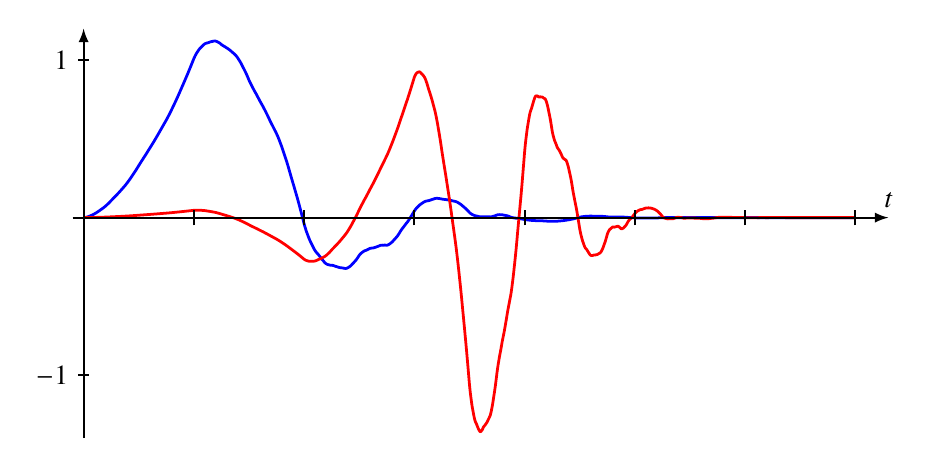
\begin{tikzpicture}[>=latex,yscale=2,xscale=1.4]

\draw[line width=1pt,color=blue] (0.00000, 0.00004)
--(0.00195, 0.00013)
--(0.00391, 0.00024)
--(0.00586, 0.00039)
--(0.00781, 0.00056)
--(0.00977, 0.00074)
--(0.01172, 0.00096)
--(0.01367, 0.00121)
--(0.01562, 0.00146)
--(0.01758, 0.00171)
--(0.01953, 0.00199)
--(0.02148, 0.00227)
--(0.02344, 0.00258)
--(0.02539, 0.00293)
--(0.02734, 0.00330)
--(0.02930, 0.00370)
--(0.03125, 0.00409)
--(0.03320, 0.00447)
--(0.03516, 0.00487)
--(0.03711, 0.00526)
--(0.03906, 0.00567)
--(0.04102, 0.00610)
--(0.04297, 0.00653)
--(0.04492, 0.00696)
--(0.04688, 0.00743)
--(0.04883, 0.00793)
--(0.05078, 0.00845)
--(0.05273, 0.00900)
--(0.05469, 0.00957)
--(0.05664, 0.01014)
--(0.05859, 0.01074)
--(0.06055, 0.01135)
--(0.06250, 0.01195)
--(0.06445, 0.01255)
--(0.06641, 0.01314)
--(0.06836, 0.01372)
--(0.07031, 0.01432)
--(0.07227, 0.01493)
--(0.07422, 0.01554)
--(0.07617, 0.01614)
--(0.07812, 0.01676)
--(0.08008, 0.01740)
--(0.08203, 0.01805)
--(0.08398, 0.01871)
--(0.08594, 0.01937)
--(0.08789, 0.02002)
--(0.08984, 0.02069)
--(0.09180, 0.02135)
--(0.09375, 0.02206)
--(0.09570, 0.02279)
--(0.09766, 0.02355)
--(0.09961, 0.02433)
--(0.10156, 0.02513)
--(0.10352, 0.02594)
--(0.10547, 0.02678)
--(0.10742, 0.02763)
--(0.10938, 0.02850)
--(0.11133, 0.02936)
--(0.11328, 0.03024)
--(0.11523, 0.03111)
--(0.11719, 0.03202)
--(0.11914, 0.03294)
--(0.12109, 0.03388)
--(0.12305, 0.03482)
--(0.12500, 0.03576)
--(0.12695, 0.03668)
--(0.12891, 0.03760)
--(0.13086, 0.03850)
--(0.13281, 0.03942)
--(0.13477, 0.04033)
--(0.13672, 0.04123)
--(0.13867, 0.04211)
--(0.14062, 0.04302)
--(0.14258, 0.04395)
--(0.14453, 0.04489)
--(0.14648, 0.04582)
--(0.14844, 0.04676)
--(0.15039, 0.04768)
--(0.15234, 0.04861)
--(0.15430, 0.04953)
--(0.15625, 0.05048)
--(0.15820, 0.05144)
--(0.16016, 0.05242)
--(0.16211, 0.05340)
--(0.16406, 0.05439)
--(0.16602, 0.05539)
--(0.16797, 0.05640)
--(0.16992, 0.05741)
--(0.17188, 0.05843)
--(0.17383, 0.05944)
--(0.17578, 0.06045)
--(0.17773, 0.06145)
--(0.17969, 0.06247)
--(0.18164, 0.06349)
--(0.18359, 0.06452)
--(0.18555, 0.06553)
--(0.18750, 0.06659)
--(0.18945, 0.06769)
--(0.19141, 0.06881)
--(0.19336, 0.06994)
--(0.19531, 0.07111)
--(0.19727, 0.07227)
--(0.19922, 0.07346)
--(0.20117, 0.07466)
--(0.20312, 0.07588)
--(0.20508, 0.07711)
--(0.20703, 0.07836)
--(0.20898, 0.07959)
--(0.21094, 0.08087)
--(0.21289, 0.08217)
--(0.21484, 0.08348)
--(0.21680, 0.08479)
--(0.21875, 0.08612)
--(0.22070, 0.08745)
--(0.22266, 0.08878)
--(0.22461, 0.09010)
--(0.22656, 0.09144)
--(0.22852, 0.09279)
--(0.23047, 0.09414)
--(0.23242, 0.09547)
--(0.23438, 0.09686)
--(0.23633, 0.09826)
--(0.23828, 0.09968)
--(0.24023, 0.10109)
--(0.24219, 0.10254)
--(0.24414, 0.10397)
--(0.24609, 0.10543)
--(0.24805, 0.10687)
--(0.25000, 0.10832)
--(0.25195, 0.10975)
--(0.25391, 0.11119)
--(0.25586, 0.11257)
--(0.25781, 0.11399)
--(0.25977, 0.11540)
--(0.26172, 0.11680)
--(0.26367, 0.11816)
--(0.26562, 0.11956)
--(0.26758, 0.12096)
--(0.26953, 0.12238)
--(0.27148, 0.12376)
--(0.27344, 0.12516)
--(0.27539, 0.12653)
--(0.27734, 0.12790)
--(0.27930, 0.12924)
--(0.28125, 0.13063)
--(0.28320, 0.13204)
--(0.28516, 0.13347)
--(0.28711, 0.13488)
--(0.28906, 0.13632)
--(0.29102, 0.13775)
--(0.29297, 0.13920)
--(0.29492, 0.14062)
--(0.29688, 0.14207)
--(0.29883, 0.14350)
--(0.30078, 0.14494)
--(0.30273, 0.14633)
--(0.30469, 0.14777)
--(0.30664, 0.14919)
--(0.30859, 0.15062)
--(0.31055, 0.15200)
--(0.31250, 0.15345)
--(0.31445, 0.15492)
--(0.31641, 0.15641)
--(0.31836, 0.15787)
--(0.32031, 0.15938)
--(0.32227, 0.16087)
--(0.32422, 0.16239)
--(0.32617, 0.16387)
--(0.32812, 0.16541)
--(0.33008, 0.16693)
--(0.33203, 0.16848)
--(0.33398, 0.16998)
--(0.33594, 0.17154)
--(0.33789, 0.17309)
--(0.33984, 0.17465)
--(0.34180, 0.17618)
--(0.34375, 0.17775)
--(0.34570, 0.17931)
--(0.34766, 0.18088)
--(0.34961, 0.18240)
--(0.35156, 0.18398)
--(0.35352, 0.18552)
--(0.35547, 0.18708)
--(0.35742, 0.18858)
--(0.35938, 0.19015)
--(0.36133, 0.19172)
--(0.36328, 0.19331)
--(0.36523, 0.19485)
--(0.36719, 0.19645)
--(0.36914, 0.19801)
--(0.37109, 0.19959)
--(0.37305, 0.20111)
--(0.37500, 0.20273)
--(0.37695, 0.20438)
--(0.37891, 0.20606)
--(0.38086, 0.20773)
--(0.38281, 0.20946)
--(0.38477, 0.21117)
--(0.38672, 0.21293)
--(0.38867, 0.21465)
--(0.39062, 0.21644)
--(0.39258, 0.21822)
--(0.39453, 0.22002)
--(0.39648, 0.22178)
--(0.39844, 0.22362)
--(0.40039, 0.22545)
--(0.40234, 0.22731)
--(0.40430, 0.22912)
--(0.40625, 0.23101)
--(0.40820, 0.23288)
--(0.41016, 0.23479)
--(0.41211, 0.23665)
--(0.41406, 0.23857)
--(0.41602, 0.24048)
--(0.41797, 0.24240)
--(0.41992, 0.24426)
--(0.42188, 0.24623)
--(0.42383, 0.24820)
--(0.42578, 0.25020)
--(0.42773, 0.25216)
--(0.42969, 0.25420)
--(0.43164, 0.25620)
--(0.43359, 0.25824)
--(0.43555, 0.26021)
--(0.43750, 0.26227)
--(0.43945, 0.26431)
--(0.44141, 0.26637)
--(0.44336, 0.26836)
--(0.44531, 0.27043)
--(0.44727, 0.27246)
--(0.44922, 0.27452)
--(0.45117, 0.27650)
--(0.45312, 0.27857)
--(0.45508, 0.28064)
--(0.45703, 0.28274)
--(0.45898, 0.28476)
--(0.46094, 0.28687)
--(0.46289, 0.28892)
--(0.46484, 0.29101)
--(0.46680, 0.29300)
--(0.46875, 0.29512)
--(0.47070, 0.29725)
--(0.47266, 0.29942)
--(0.47461, 0.30154)
--(0.47656, 0.30374)
--(0.47852, 0.30590)
--(0.48047, 0.30811)
--(0.48242, 0.31024)
--(0.48438, 0.31247)
--(0.48633, 0.31468)
--(0.48828, 0.31692)
--(0.49023, 0.31908)
--(0.49219, 0.32134)
--(0.49414, 0.32356)
--(0.49609, 0.32581)
--(0.49805, 0.32796)
--(0.50000, 0.33022)
--(0.50195, 0.33244)
--(0.50391, 0.33468)
--(0.50586, 0.33682)
--(0.50781, 0.33905)
--(0.50977, 0.34122)
--(0.51172, 0.34341)
--(0.51367, 0.34548)
--(0.51562, 0.34767)
--(0.51758, 0.34984)
--(0.51953, 0.35204)
--(0.52148, 0.35415)
--(0.52344, 0.35634)
--(0.52539, 0.35846)
--(0.52734, 0.36060)
--(0.52930, 0.36263)
--(0.53125, 0.36479)
--(0.53320, 0.36694)
--(0.53516, 0.36913)
--(0.53711, 0.37123)
--(0.53906, 0.37343)
--(0.54102, 0.37556)
--(0.54297, 0.37774)
--(0.54492, 0.37980)
--(0.54688, 0.38198)
--(0.54883, 0.38411)
--(0.55078, 0.38627)
--(0.55273, 0.38831)
--(0.55469, 0.39045)
--(0.55664, 0.39253)
--(0.55859, 0.39464)
--(0.56055, 0.39661)
--(0.56250, 0.39875)
--(0.56445, 0.40090)
--(0.56641, 0.40310)
--(0.56836, 0.40521)
--(0.57031, 0.40744)
--(0.57227, 0.40960)
--(0.57422, 0.41182)
--(0.57617, 0.41392)
--(0.57812, 0.41616)
--(0.58008, 0.41836)
--(0.58203, 0.42061)
--(0.58398, 0.42273)
--(0.58594, 0.42499)
--(0.58789, 0.42719)
--(0.58984, 0.42943)
--(0.59180, 0.43154)
--(0.59375, 0.43379)
--(0.59570, 0.43600)
--(0.59766, 0.43826)
--(0.59961, 0.44039)
--(0.60156, 0.44263)
--(0.60352, 0.44481)
--(0.60547, 0.44701)
--(0.60742, 0.44907)
--(0.60938, 0.45129)
--(0.61133, 0.45349)
--(0.61328, 0.45573)
--(0.61523, 0.45785)
--(0.61719, 0.46008)
--(0.61914, 0.46224)
--(0.62109, 0.46443)
--(0.62305, 0.46648)
--(0.62500, 0.46872)
--(0.62695, 0.47095)
--(0.62891, 0.47324)
--(0.63086, 0.47543)
--(0.63281, 0.47775)
--(0.63477, 0.48000)
--(0.63672, 0.48232)
--(0.63867, 0.48450)
--(0.64062, 0.48685)
--(0.64258, 0.48915)
--(0.64453, 0.49150)
--(0.64648, 0.49371)
--(0.64844, 0.49607)
--(0.65039, 0.49837)
--(0.65234, 0.50071)
--(0.65430, 0.50290)
--(0.65625, 0.50528)
--(0.65820, 0.50762)
--(0.66016, 0.51003)
--(0.66211, 0.51230)
--(0.66406, 0.51471)
--(0.66602, 0.51705)
--(0.66797, 0.51943)
--(0.66992, 0.52166)
--(0.67188, 0.52407)
--(0.67383, 0.52645)
--(0.67578, 0.52889)
--(0.67773, 0.53119)
--(0.67969, 0.53364)
--(0.68164, 0.53601)
--(0.68359, 0.53842)
--(0.68555, 0.54067)
--(0.68750, 0.54311)
--(0.68945, 0.54552)
--(0.69141, 0.54797)
--(0.69336, 0.55028)
--(0.69531, 0.55275)
--(0.69727, 0.55512)
--(0.69922, 0.55754)
--(0.70117, 0.55978)
--(0.70312, 0.56222)
--(0.70508, 0.56462)
--(0.70703, 0.56707)
--(0.70898, 0.56936)
--(0.71094, 0.57180)
--(0.71289, 0.57415)
--(0.71484, 0.57654)
--(0.71680, 0.57874)
--(0.71875, 0.58117)
--(0.72070, 0.58358)
--(0.72266, 0.58605)
--(0.72461, 0.58838)
--(0.72656, 0.59086)
--(0.72852, 0.59326)
--(0.73047, 0.59571)
--(0.73242, 0.59799)
--(0.73438, 0.60047)
--(0.73633, 0.60289)
--(0.73828, 0.60537)
--(0.74023, 0.60767)
--(0.74219, 0.61014)
--(0.74414, 0.61252)
--(0.74609, 0.61495)
--(0.74805, 0.61718)
--(0.75000, 0.61968)
--(0.75195, 0.62217)
--(0.75391, 0.62476)
--(0.75586, 0.62722)
--(0.75781, 0.62985)
--(0.75977, 0.63240)
--(0.76172, 0.63503)
--(0.76367, 0.63750)
--(0.76562, 0.64018)
--(0.76758, 0.64282)
--(0.76953, 0.64553)
--(0.77148, 0.64806)
--(0.77344, 0.65080)
--(0.77539, 0.65347)
--(0.77734, 0.65620)
--(0.77930, 0.65874)
--(0.78125, 0.66152)
--(0.78320, 0.66425)
--(0.78516, 0.66706)
--(0.78711, 0.66969)
--(0.78906, 0.67252)
--(0.79102, 0.67525)
--(0.79297, 0.67804)
--(0.79492, 0.68063)
--(0.79688, 0.68347)
--(0.79883, 0.68628)
--(0.80078, 0.68917)
--(0.80273, 0.69189)
--(0.80469, 0.69480)
--(0.80664, 0.69760)
--(0.80859, 0.70048)
--(0.81055, 0.70315)
--(0.81250, 0.70607)
--(0.81445, 0.70896)
--(0.81641, 0.71192)
--(0.81836, 0.71470)
--(0.82031, 0.71769)
--(0.82227, 0.72057)
--(0.82422, 0.72352)
--(0.82617, 0.72625)
--(0.82812, 0.72924)
--(0.83008, 0.73218)
--(0.83203, 0.73519)
--(0.83398, 0.73801)
--(0.83594, 0.74103)
--(0.83789, 0.74393)
--(0.83984, 0.74690)
--(0.84180, 0.74963)
--(0.84375, 0.75266)
--(0.84570, 0.75568)
--(0.84766, 0.75878)
--(0.84961, 0.76171)
--(0.85156, 0.76485)
--(0.85352, 0.76787)
--(0.85547, 0.77098)
--(0.85742, 0.77387)
--(0.85938, 0.77703)
--(0.86133, 0.78013)
--(0.86328, 0.78330)
--(0.86523, 0.78626)
--(0.86719, 0.78945)
--(0.86914, 0.79253)
--(0.87109, 0.79568)
--(0.87305, 0.79858)
--(0.87500, 0.80177)
--(0.87695, 0.80491)
--(0.87891, 0.80813)
--(0.88086, 0.81115)
--(0.88281, 0.81438)
--(0.88477, 0.81749)
--(0.88672, 0.82066)
--(0.88867, 0.82358)
--(0.89062, 0.82679)
--(0.89258, 0.82995)
--(0.89453, 0.83318)
--(0.89648, 0.83618)
--(0.89844, 0.83941)
--(0.90039, 0.84250)
--(0.90234, 0.84566)
--(0.90430, 0.84855)
--(0.90625, 0.85176)
--(0.90820, 0.85494)
--(0.91016, 0.85821)
--(0.91211, 0.86126)
--(0.91406, 0.86456)
--(0.91602, 0.86771)
--(0.91797, 0.87095)
--(0.91992, 0.87393)
--(0.92188, 0.87720)
--(0.92383, 0.88039)
--(0.92578, 0.88367)
--(0.92773, 0.88669)
--(0.92969, 0.88996)
--(0.93164, 0.89309)
--(0.93359, 0.89629)
--(0.93555, 0.89921)
--(0.93750, 0.90248)
--(0.93945, 0.90573)
--(0.94141, 0.90910)
--(0.94336, 0.91225)
--(0.94531, 0.91566)
--(0.94727, 0.91892)
--(0.94922, 0.92230)
--(0.95117, 0.92541)
--(0.95312, 0.92883)
--(0.95508, 0.93218)
--(0.95703, 0.93562)
--(0.95898, 0.93880)
--(0.96094, 0.94226)
--(0.96289, 0.94559)
--(0.96484, 0.94900)
--(0.96680, 0.95212)
--(0.96875, 0.95558)
--(0.97070, 0.95898)
--(0.97266, 0.96249)
--(0.97461, 0.96575)
--(0.97656, 0.96927)
--(0.97852, 0.97263)
--(0.98047, 0.97609)
--(0.98242, 0.97924)
--(0.98438, 0.98274)
--(0.98633, 0.98618)
--(0.98828, 0.98971)
--(0.99023, 0.99298)
--(0.99219, 0.99652)
--(0.99414, 0.99989)
--(0.99609, 1.00336)
--(0.99805, 1.00651)
--(1.00000, 1.00988)
--(1.00195, 1.01305)
--(1.00391, 1.01623)
--(1.00586, 1.01901)
--(1.00781, 1.02203)
--(1.00977, 1.02483)
--(1.01172, 1.02760)
--(1.01367, 1.02995)
--(1.01562, 1.03263)
--(1.01758, 1.03522)
--(1.01953, 1.03785)
--(1.02148, 1.04015)
--(1.02344, 1.04263)
--(1.02539, 1.04481)
--(1.02734, 1.04700)
--(1.02930, 1.04878)
--(1.03125, 1.05096)
--(1.03320, 1.05312)
--(1.03516, 1.05536)
--(1.03711, 1.05733)
--(1.03906, 1.05953)
--(1.04102, 1.06150)
--(1.04297, 1.06356)
--(1.04492, 1.06529)
--(1.04688, 1.06725)
--(1.04883, 1.06901)
--(1.05078, 1.07079)
--(1.05273, 1.07216)
--(1.05469, 1.07380)
--(1.05664, 1.07523)
--(1.05859, 1.07666)
--(1.06055, 1.07767)
--(1.06250, 1.07914)
--(1.06445, 1.08060)
--(1.06641, 1.08219)
--(1.06836, 1.08354)
--(1.07031, 1.08515)
--(1.07227, 1.08652)
--(1.07422, 1.08803)
--(1.07617, 1.08921)
--(1.07812, 1.09071)
--(1.08008, 1.09206)
--(1.08203, 1.09348)
--(1.08398, 1.09454)
--(1.08594, 1.09592)
--(1.08789, 1.09714)
--(1.08984, 1.09842)
--(1.09180, 1.09933)
--(1.09375, 1.10054)
--(1.09570, 1.10157)
--(1.09766, 1.10264)
--(1.09961, 1.10332)
--(1.10156, 1.10426)
--(1.10352, 1.10497)
--(1.10547, 1.10568)
--(1.10742, 1.10596)
--(1.10938, 1.10662)
--(1.11133, 1.10720)
--(1.11328, 1.10783)
--(1.11523, 1.10814)
--(1.11719, 1.10866)
--(1.11914, 1.10893)
--(1.12109, 1.10924)
--(1.12305, 1.10914)
--(1.12500, 1.10953)
--(1.12695, 1.10996)
--(1.12891, 1.11053)
--(1.13086, 1.11087)
--(1.13281, 1.11152)
--(1.13477, 1.11197)
--(1.13672, 1.11259)
--(1.13867, 1.11292)
--(1.14062, 1.11357)
--(1.14258, 1.11406)
--(1.14453, 1.11465)
--(1.14648, 1.11487)
--(1.14844, 1.11546)
--(1.15039, 1.11591)
--(1.15234, 1.11644)
--(1.15430, 1.11663)
--(1.15625, 1.11717)
--(1.15820, 1.11758)
--(1.16016, 1.11809)
--(1.16211, 1.11826)
--(1.16406, 1.11872)
--(1.16602, 1.11898)
--(1.16797, 1.11929)
--(1.16992, 1.11922)
--(1.17188, 1.11957)
--(1.17383, 1.11986)
--(1.17578, 1.12025)
--(1.17773, 1.12035)
--(1.17969, 1.12073)
--(1.18164, 1.12089)
--(1.18359, 1.12115)
--(1.18555, 1.12104)
--(1.18750, 1.12125)
--(1.18945, 1.12128)
--(1.19141, 1.12136)
--(1.19336, 1.12106)
--(1.19531, 1.12102)
--(1.19727, 1.12077)
--(1.19922, 1.12053)
--(1.20117, 1.11988)
--(1.20312, 1.11958)
--(1.20508, 1.11917)
--(1.20703, 1.11882)
--(1.20898, 1.11813)
--(1.21094, 1.11765)
--(1.21289, 1.11692)
--(1.21484, 1.11621)
--(1.21680, 1.11509)
--(1.21875, 1.11440)
--(1.22070, 1.11369)
--(1.22266, 1.11307)
--(1.22461, 1.11218)
--(1.22656, 1.11156)
--(1.22852, 1.11071)
--(1.23047, 1.10996)
--(1.23242, 1.10887)
--(1.23438, 1.10808)
--(1.23633, 1.10712)
--(1.23828, 1.10621)
--(1.24023, 1.10492)
--(1.24219, 1.10392)
--(1.24414, 1.10273)
--(1.24609, 1.10157)
--(1.24805, 1.10002)
--(1.25000, 1.09896)
--(1.25195, 1.09794)
--(1.25391, 1.09708)
--(1.25586, 1.09602)
--(1.25781, 1.09525)
--(1.25977, 1.09429)
--(1.26172, 1.09351)
--(1.26367, 1.09243)
--(1.26562, 1.09171)
--(1.26758, 1.09088)
--(1.26953, 1.09016)
--(1.27148, 1.08911)
--(1.27344, 1.08843)
--(1.27539, 1.08763)
--(1.27734, 1.08693)
--(1.27930, 1.08592)
--(1.28125, 1.08525)
--(1.28320, 1.08444)
--(1.28516, 1.08372)
--(1.28711, 1.08267)
--(1.28906, 1.08192)
--(1.29102, 1.08099)
--(1.29297, 1.08011)
--(1.29492, 1.07886)
--(1.29688, 1.07804)
--(1.29883, 1.07718)
--(1.30078, 1.07644)
--(1.30273, 1.07544)
--(1.30469, 1.07470)
--(1.30664, 1.07377)
--(1.30859, 1.07293)
--(1.31055, 1.07176)
--(1.31250, 1.07094)
--(1.31445, 1.07002)
--(1.31641, 1.06918)
--(1.31836, 1.06802)
--(1.32031, 1.06714)
--(1.32227, 1.06609)
--(1.32422, 1.06510)
--(1.32617, 1.06376)
--(1.32812, 1.06277)
--(1.33008, 1.06169)
--(1.33203, 1.06068)
--(1.33398, 1.05937)
--(1.33594, 1.05831)
--(1.33789, 1.05706)
--(1.33984, 1.05586)
--(1.34180, 1.05429)
--(1.34375, 1.05315)
--(1.34570, 1.05200)
--(1.34766, 1.05097)
--(1.34961, 1.04969)
--(1.35156, 1.04869)
--(1.35352, 1.04751)
--(1.35547, 1.04644)
--(1.35742, 1.04507)
--(1.35938, 1.04402)
--(1.36133, 1.04286)
--(1.36328, 1.04178)
--(1.36523, 1.04038)
--(1.36719, 1.03927)
--(1.36914, 1.03802)
--(1.37109, 1.03683)
--(1.37305, 1.03530)
--(1.37500, 1.03406)
--(1.37695, 1.03266)
--(1.37891, 1.03132)
--(1.38086, 1.02962)
--(1.38281, 1.02816)
--(1.38477, 1.02649)
--(1.38672, 1.02483)
--(1.38867, 1.02278)
--(1.39062, 1.02107)
--(1.39258, 1.01928)
--(1.39453, 1.01753)
--(1.39648, 1.01548)
--(1.39844, 1.01363)
--(1.40039, 1.01154)
--(1.40234, 1.00947)
--(1.40430, 1.00703)
--(1.40625, 1.00496)
--(1.40820, 1.00285)
--(1.41016, 1.00081)
--(1.41211, 0.99850)
--(1.41406, 0.99643)
--(1.41602, 0.99415)
--(1.41797, 0.99194)
--(1.41992, 0.98941)
--(1.42188, 0.98714)
--(1.42383, 0.98472)
--(1.42578, 0.98233)
--(1.42773, 0.97960)
--(1.42969, 0.97710)
--(1.43164, 0.97442)
--(1.43359, 0.97176)
--(1.43555, 0.96873)
--(1.43750, 0.96611)
--(1.43945, 0.96349)
--(1.44141, 0.96099)
--(1.44336, 0.95828)
--(1.44531, 0.95580)
--(1.44727, 0.95314)
--(1.44922, 0.95059)
--(1.45117, 0.94777)
--(1.45312, 0.94523)
--(1.45508, 0.94257)
--(1.45703, 0.93998)
--(1.45898, 0.93709)
--(1.46094, 0.93448)
--(1.46289, 0.93174)
--(1.46484, 0.92905)
--(1.46680, 0.92606)
--(1.46875, 0.92334)
--(1.47070, 0.92050)
--(1.47266, 0.91770)
--(1.47461, 0.91461)
--(1.47656, 0.91173)
--(1.47852, 0.90868)
--(1.48047, 0.90564)
--(1.48242, 0.90227)
--(1.48438, 0.89922)
--(1.48633, 0.89610)
--(1.48828, 0.89305)
--(1.49023, 0.88974)
--(1.49219, 0.88663)
--(1.49414, 0.88332)
--(1.49609, 0.88005)
--(1.49805, 0.87648)
--(1.50000, 0.87333)
--(1.50195, 0.87027)
--(1.50391, 0.86736)
--(1.50586, 0.86431)
--(1.50781, 0.86152)
--(1.50977, 0.85860)
--(1.51172, 0.85586)
--(1.51367, 0.85293)
--(1.51562, 0.85026)
--(1.51758, 0.84750)
--(1.51953, 0.84483)
--(1.52148, 0.84191)
--(1.52344, 0.83930)
--(1.52539, 0.83664)
--(1.52734, 0.83407)
--(1.52930, 0.83127)
--(1.53125, 0.82875)
--(1.53320, 0.82615)
--(1.53516, 0.82364)
--(1.53711, 0.82090)
--(1.53906, 0.81840)
--(1.54102, 0.81578)
--(1.54297, 0.81322)
--(1.54492, 0.81040)
--(1.54688, 0.80793)
--(1.54883, 0.80547)
--(1.55078, 0.80311)
--(1.55273, 0.80059)
--(1.55469, 0.79829)
--(1.55664, 0.79586)
--(1.55859, 0.79354)
--(1.56055, 0.79099)
--(1.56250, 0.78867)
--(1.56445, 0.78624)
--(1.56641, 0.78386)
--(1.56836, 0.78121)
--(1.57031, 0.77878)
--(1.57227, 0.77623)
--(1.57422, 0.77370)
--(1.57617, 0.77090)
--(1.57812, 0.76838)
--(1.58008, 0.76582)
--(1.58203, 0.76332)
--(1.58398, 0.76061)
--(1.58594, 0.75807)
--(1.58789, 0.75537)
--(1.58984, 0.75271)
--(1.59180, 0.74979)
--(1.59375, 0.74722)
--(1.59570, 0.74468)
--(1.59766, 0.74225)
--(1.59961, 0.73969)
--(1.60156, 0.73733)
--(1.60352, 0.73485)
--(1.60547, 0.73249)
--(1.60742, 0.72995)
--(1.60938, 0.72762)
--(1.61133, 0.72520)
--(1.61328, 0.72284)
--(1.61523, 0.72026)
--(1.61719, 0.71791)
--(1.61914, 0.71548)
--(1.62109, 0.71309)
--(1.62305, 0.71049)
--(1.62500, 0.70810)
--(1.62695, 0.70563)
--(1.62891, 0.70320)
--(1.63086, 0.70055)
--(1.63281, 0.69808)
--(1.63477, 0.69547)
--(1.63672, 0.69288)
--(1.63867, 0.69004)
--(1.64062, 0.68744)
--(1.64258, 0.68482)
--(1.64453, 0.68224)
--(1.64648, 0.67947)
--(1.64844, 0.67685)
--(1.65039, 0.67408)
--(1.65234, 0.67135)
--(1.65430, 0.66838)
--(1.65625, 0.66567)
--(1.65820, 0.66294)
--(1.66016, 0.66027)
--(1.66211, 0.65742)
--(1.66406, 0.65474)
--(1.66602, 0.65194)
--(1.66797, 0.64921)
--(1.66992, 0.64626)
--(1.67188, 0.64351)
--(1.67383, 0.64067)
--(1.67578, 0.63787)
--(1.67773, 0.63485)
--(1.67969, 0.63200)
--(1.68164, 0.62904)
--(1.68359, 0.62611)
--(1.68555, 0.62295)
--(1.68750, 0.62008)
--(1.68945, 0.61725)
--(1.69141, 0.61451)
--(1.69336, 0.61166)
--(1.69531, 0.60898)
--(1.69727, 0.60620)
--(1.69922, 0.60352)
--(1.70117, 0.60069)
--(1.70312, 0.59805)
--(1.70508, 0.59535)
--(1.70703, 0.59271)
--(1.70898, 0.58990)
--(1.71094, 0.58728)
--(1.71289, 0.58461)
--(1.71484, 0.58200)
--(1.71680, 0.57921)
--(1.71875, 0.57661)
--(1.72070, 0.57393)
--(1.72266, 0.57131)
--(1.72461, 0.56851)
--(1.72656, 0.56586)
--(1.72852, 0.56312)
--(1.73047, 0.56041)
--(1.73242, 0.55750)
--(1.73438, 0.55481)
--(1.73633, 0.55212)
--(1.73828, 0.54947)
--(1.74023, 0.54670)
--(1.74219, 0.54406)
--(1.74414, 0.54131)
--(1.74609, 0.53862)
--(1.74805, 0.53575)
--(1.75000, 0.53298)
--(1.75195, 0.53009)
--(1.75391, 0.52718)
--(1.75586, 0.52404)
--(1.75781, 0.52102)
--(1.75977, 0.51788)
--(1.76172, 0.51470)
--(1.76367, 0.51128)
--(1.76562, 0.50803)
--(1.76758, 0.50472)
--(1.76953, 0.50142)
--(1.77148, 0.49795)
--(1.77344, 0.49454)
--(1.77539, 0.49095)
--(1.77734, 0.48736)
--(1.77930, 0.48355)
--(1.78125, 0.47994)
--(1.78320, 0.47634)
--(1.78516, 0.47277)
--(1.78711, 0.46908)
--(1.78906, 0.46549)
--(1.79102, 0.46178)
--(1.79297, 0.45811)
--(1.79492, 0.45429)
--(1.79688, 0.45055)
--(1.79883, 0.44669)
--(1.80078, 0.44282)
--(1.80273, 0.43875)
--(1.80469, 0.43478)
--(1.80664, 0.43073)
--(1.80859, 0.42665)
--(1.81055, 0.42238)
--(1.81250, 0.41830)
--(1.81445, 0.41424)
--(1.81641, 0.41022)
--(1.81836, 0.40611)
--(1.82031, 0.40209)
--(1.82227, 0.39796)
--(1.82422, 0.39389)
--(1.82617, 0.38969)
--(1.82812, 0.38559)
--(1.83008, 0.38143)
--(1.83203, 0.37728)
--(1.83398, 0.37299)
--(1.83594, 0.36882)
--(1.83789, 0.36458)
--(1.83984, 0.36036)
--(1.84180, 0.35600)
--(1.84375, 0.35171)
--(1.84570, 0.34733)
--(1.84766, 0.34294)
--(1.84961, 0.33839)
--(1.85156, 0.33391)
--(1.85352, 0.32934)
--(1.85547, 0.32473)
--(1.85742, 0.31997)
--(1.85938, 0.31531)
--(1.86133, 0.31063)
--(1.86328, 0.30595)
--(1.86523, 0.30117)
--(1.86719, 0.29643)
--(1.86914, 0.29157)
--(1.87109, 0.28672)
--(1.87305, 0.28173)
--(1.87500, 0.27691)
--(1.87695, 0.27216)
--(1.87891, 0.26746)
--(1.88086, 0.26275)
--(1.88281, 0.25811)
--(1.88477, 0.25342)
--(1.88672, 0.24881)
--(1.88867, 0.24416)
--(1.89062, 0.23956)
--(1.89258, 0.23491)
--(1.89453, 0.23027)
--(1.89648, 0.22555)
--(1.89844, 0.22092)
--(1.90039, 0.21631)
--(1.90234, 0.21171)
--(1.90430, 0.20706)
--(1.90625, 0.20244)
--(1.90820, 0.19778)
--(1.91016, 0.19313)
--(1.91211, 0.18839)
--(1.91406, 0.18370)
--(1.91602, 0.17898)
--(1.91797, 0.17425)
--(1.91992, 0.16943)
--(1.92188, 0.16471)
--(1.92383, 0.16001)
--(1.92578, 0.15534)
--(1.92773, 0.15064)
--(1.92969, 0.14597)
--(1.93164, 0.14126)
--(1.93359, 0.13658)
--(1.93555, 0.13185)
--(1.93750, 0.12710)
--(1.93945, 0.12227)
--(1.94141, 0.11741)
--(1.94336, 0.11245)
--(1.94531, 0.10751)
--(1.94727, 0.10253)
--(1.94922, 0.09750)
--(1.95117, 0.09239)
--(1.95312, 0.08731)
--(1.95508, 0.08222)
--(1.95703, 0.07711)
--(1.95898, 0.07196)
--(1.96094, 0.06678)
--(1.96289, 0.06153)
--(1.96484, 0.05626)
--(1.96680, 0.05092)
--(1.96875, 0.04564)
--(1.97070, 0.04040)
--(1.97266, 0.03516)
--(1.97461, 0.02992)
--(1.97656, 0.02468)
--(1.97852, 0.01942)
--(1.98047, 0.01417)
--(1.98242, 0.00892)
--(1.98438, 0.00363)
--(1.98633, -0.00171)
--(1.98828, -0.00707)
--(1.99023, -0.01248)
--(1.99219, -0.01789)
--(1.99414, -0.02329)
--(1.99609, -0.02872)
--(1.99805, -0.03417)
--(2.00000, -0.03941)
--(2.00195, -0.04442)
--(2.00391, -0.04930)
--(2.00586, -0.05398)
--(2.00781, -0.05861)
--(2.00977, -0.06319)
--(2.01172, -0.06759)
--(2.01367, -0.07182)
--(2.01562, -0.07606)
--(2.01758, -0.08028)
--(2.01953, -0.08444)
--(2.02148, -0.08854)
--(2.02344, -0.09250)
--(2.02539, -0.09627)
--(2.02734, -0.09996)
--(2.02930, -0.10351)
--(2.03125, -0.10713)
--(2.03320, -0.11082)
--(2.03516, -0.11448)
--(2.03711, -0.11813)
--(2.03906, -0.12175)
--(2.04102, -0.12528)
--(2.04297, -0.12883)
--(2.04492, -0.13234)
--(2.04688, -0.13573)
--(2.04883, -0.13894)
--(2.05078, -0.14206)
--(2.05273, -0.14500)
--(2.05469, -0.14795)
--(2.05664, -0.15085)
--(2.05859, -0.15366)
--(2.06055, -0.15633)
--(2.06250, -0.15912)
--(2.06445, -0.16196)
--(2.06641, -0.16483)
--(2.06836, -0.16772)
--(2.07031, -0.17059)
--(2.07227, -0.17338)
--(2.07422, -0.17622)
--(2.07617, -0.17902)
--(2.07812, -0.18180)
--(2.08008, -0.18452)
--(2.08203, -0.18720)
--(2.08398, -0.18979)
--(2.08594, -0.19244)
--(2.08789, -0.19508)
--(2.08984, -0.19772)
--(2.09180, -0.20028)
--(2.09375, -0.20276)
--(2.09570, -0.20506)
--(2.09766, -0.20730)
--(2.09961, -0.20936)
--(2.10156, -0.21142)
--(2.10352, -0.21338)
--(2.10547, -0.21524)
--(2.10742, -0.21693)
--(2.10938, -0.21868)
--(2.11133, -0.22043)
--(2.11328, -0.22215)
--(2.11523, -0.22379)
--(2.11719, -0.22539)
--(2.11914, -0.22684)
--(2.12109, -0.22827)
--(2.12305, -0.22956)
--(2.12500, -0.23105)
--(2.12695, -0.23265)
--(2.12891, -0.23432)
--(2.13086, -0.23603)
--(2.13281, -0.23780)
--(2.13477, -0.23953)
--(2.13672, -0.24138)
--(2.13867, -0.24324)
--(2.14062, -0.24510)
--(2.14258, -0.24686)
--(2.14453, -0.24865)
--(2.14648, -0.25031)
--(2.14844, -0.25212)
--(2.15039, -0.25398)
--(2.15234, -0.25584)
--(2.15430, -0.25766)
--(2.15625, -0.25949)
--(2.15820, -0.26122)
--(2.16016, -0.26295)
--(2.16211, -0.26457)
--(2.16406, -0.26624)
--(2.16602, -0.26786)
--(2.16797, -0.26945)
--(2.16992, -0.27091)
--(2.17188, -0.27253)
--(2.17383, -0.27418)
--(2.17578, -0.27587)
--(2.17773, -0.27753)
--(2.17969, -0.27923)
--(2.18164, -0.28086)
--(2.18359, -0.28252)
--(2.18555, -0.28411)
--(2.18750, -0.28565)
--(2.18945, -0.28701)
--(2.19141, -0.28831)
--(2.19336, -0.28939)
--(2.19531, -0.29051)
--(2.19727, -0.29155)
--(2.19922, -0.29249)
--(2.20117, -0.29324)
--(2.20312, -0.29407)
--(2.20508, -0.29486)
--(2.20703, -0.29563)
--(2.20898, -0.29629)
--(2.21094, -0.29691)
--(2.21289, -0.29737)
--(2.21484, -0.29779)
--(2.21680, -0.29803)
--(2.21875, -0.29843)
--(2.22070, -0.29888)
--(2.22266, -0.29934)
--(2.22461, -0.29976)
--(2.22656, -0.30021)
--(2.22852, -0.30058)
--(2.23047, -0.30100)
--(2.23242, -0.30133)
--(2.23438, -0.30166)
--(2.23633, -0.30186)
--(2.23828, -0.30203)
--(2.24023, -0.30202)
--(2.24219, -0.30210)
--(2.24414, -0.30212)
--(2.24609, -0.30211)
--(2.24805, -0.30196)
--(2.25000, -0.30202)
--(2.25195, -0.30218)
--(2.25391, -0.30242)
--(2.25586, -0.30268)
--(2.25781, -0.30302)
--(2.25977, -0.30330)
--(2.26172, -0.30369)
--(2.26367, -0.30405)
--(2.26562, -0.30449)
--(2.26758, -0.30490)
--(2.26953, -0.30534)
--(2.27148, -0.30570)
--(2.27344, -0.30621)
--(2.27539, -0.30675)
--(2.27734, -0.30735)
--(2.27930, -0.30788)
--(2.28125, -0.30846)
--(2.28320, -0.30892)
--(2.28516, -0.30940)
--(2.28711, -0.30974)
--(2.28906, -0.31016)
--(2.29102, -0.31055)
--(2.29297, -0.31091)
--(2.29492, -0.31114)
--(2.29688, -0.31155)
--(2.29883, -0.31200)
--(2.30078, -0.31251)
--(2.30273, -0.31298)
--(2.30469, -0.31351)
--(2.30664, -0.31396)
--(2.30859, -0.31447)
--(2.31055, -0.31489)
--(2.31250, -0.31537)
--(2.31445, -0.31578)
--(2.31641, -0.31618)
--(2.31836, -0.31645)
--(2.32031, -0.31680)
--(2.32227, -0.31711)
--(2.32422, -0.31740)
--(2.32617, -0.31756)
--(2.32812, -0.31783)
--(2.33008, -0.31807)
--(2.33203, -0.31833)
--(2.33398, -0.31849)
--(2.33594, -0.31870)
--(2.33789, -0.31882)
--(2.33984, -0.31894)
--(2.34180, -0.31894)
--(2.34375, -0.31910)
--(2.34570, -0.31931)
--(2.34766, -0.31956)
--(2.34961, -0.31976)
--(2.35156, -0.32006)
--(2.35352, -0.32029)
--(2.35547, -0.32059)
--(2.35742, -0.32082)
--(2.35938, -0.32112)
--(2.36133, -0.32136)
--(2.36328, -0.32163)
--(2.36523, -0.32178)
--(2.36719, -0.32204)
--(2.36914, -0.32227)
--(2.37109, -0.32252)
--(2.37305, -0.32267)
--(2.37500, -0.32281)
--(2.37695, -0.32279)
--(2.37891, -0.32272)
--(2.38086, -0.32246)
--(2.38281, -0.32223)
--(2.38477, -0.32190)
--(2.38672, -0.32149)
--(2.38867, -0.32087)
--(2.39062, -0.32037)
--(2.39258, -0.31984)
--(2.39453, -0.31929)
--(2.39648, -0.31864)
--(2.39844, -0.31797)
--(2.40039, -0.31714)
--(2.40234, -0.31629)
--(2.40430, -0.31526)
--(2.40625, -0.31436)
--(2.40820, -0.31346)
--(2.41016, -0.31256)
--(2.41211, -0.31157)
--(2.41406, -0.31063)
--(2.41602, -0.30959)
--(2.41797, -0.30857)
--(2.41992, -0.30744)
--(2.42188, -0.30631)
--(2.42383, -0.30507)
--(2.42578, -0.30378)
--(2.42773, -0.30233)
--(2.42969, -0.30093)
--(2.43164, -0.29945)
--(2.43359, -0.29793)
--(2.43555, -0.29625)
--(2.43750, -0.29474)
--(2.43945, -0.29328)
--(2.44141, -0.29187)
--(2.44336, -0.29043)
--(2.44531, -0.28905)
--(2.44727, -0.28759)
--(2.44922, -0.28619)
--(2.45117, -0.28472)
--(2.45312, -0.28331)
--(2.45508, -0.28183)
--(2.45703, -0.28036)
--(2.45898, -0.27877)
--(2.46094, -0.27729)
--(2.46289, -0.27579)
--(2.46484, -0.27430)
--(2.46680, -0.27272)
--(2.46875, -0.27116)
--(2.47070, -0.26948)
--(2.47266, -0.26778)
--(2.47461, -0.26593)
--(2.47656, -0.26412)
--(2.47852, -0.26225)
--(2.48047, -0.26032)
--(2.48242, -0.25824)
--(2.48438, -0.25627)
--(2.48633, -0.25430)
--(2.48828, -0.25233)
--(2.49023, -0.25030)
--(2.49219, -0.24827)
--(2.49414, -0.24615)
--(2.49609, -0.24402)
--(2.49805, -0.24179)
--(2.50000, -0.23980)
--(2.50195, -0.23799)
--(2.50391, -0.23628)
--(2.50586, -0.23466)
--(2.50781, -0.23313)
--(2.50977, -0.23161)
--(2.51172, -0.23025)
--(2.51367, -0.22894)
--(2.51562, -0.22768)
--(2.51758, -0.22637)
--(2.51953, -0.22512)
--(2.52148, -0.22381)
--(2.52344, -0.22268)
--(2.52539, -0.22165)
--(2.52734, -0.22068)
--(2.52930, -0.21971)
--(2.53125, -0.21879)
--(2.53320, -0.21781)
--(2.53516, -0.21687)
--(2.53711, -0.21586)
--(2.53906, -0.21495)
--(2.54102, -0.21404)
--(2.54297, -0.21315)
--(2.54492, -0.21218)
--(2.54688, -0.21140)
--(2.54883, -0.21072)
--(2.55078, -0.21013)
--(2.55273, -0.20958)
--(2.55469, -0.20910)
--(2.55664, -0.20860)
--(2.55859, -0.20820)
--(2.56055, -0.20779)
--(2.56250, -0.20736)
--(2.56445, -0.20682)
--(2.56641, -0.20626)
--(2.56836, -0.20555)
--(2.57031, -0.20493)
--(2.57227, -0.20429)
--(2.57422, -0.20361)
--(2.57617, -0.20282)
--(2.57812, -0.20214)
--(2.58008, -0.20148)
--(2.58203, -0.20085)
--(2.58398, -0.20020)
--(2.58594, -0.19954)
--(2.58789, -0.19880)
--(2.58984, -0.19807)
--(2.59180, -0.19726)
--(2.59375, -0.19663)
--(2.59570, -0.19612)
--(2.59766, -0.19568)
--(2.59961, -0.19528)
--(2.60156, -0.19496)
--(2.60352, -0.19463)
--(2.60547, -0.19441)
--(2.60742, -0.19421)
--(2.60938, -0.19403)
--(2.61133, -0.19379)
--(2.61328, -0.19359)
--(2.61523, -0.19331)
--(2.61719, -0.19315)
--(2.61914, -0.19303)
--(2.62109, -0.19293)
--(2.62305, -0.19279)
--(2.62500, -0.19266)
--(2.62695, -0.19242)
--(2.62891, -0.19217)
--(2.63086, -0.19181)
--(2.63281, -0.19149)
--(2.63477, -0.19112)
--(2.63672, -0.19070)
--(2.63867, -0.19016)
--(2.64062, -0.18973)
--(2.64258, -0.18932)
--(2.64453, -0.18893)
--(2.64648, -0.18850)
--(2.64844, -0.18807)
--(2.65039, -0.18755)
--(2.65234, -0.18703)
--(2.65430, -0.18644)
--(2.65625, -0.18594)
--(2.65820, -0.18546)
--(2.66016, -0.18500)
--(2.66211, -0.18450)
--(2.66406, -0.18405)
--(2.66602, -0.18357)
--(2.66797, -0.18312)
--(2.66992, -0.18262)
--(2.67188, -0.18214)
--(2.67383, -0.18160)
--(2.67578, -0.18106)
--(2.67773, -0.18042)
--(2.67969, -0.17984)
--(2.68164, -0.17924)
--(2.68359, -0.17862)
--(2.68555, -0.17793)
--(2.68750, -0.17739)
--(2.68945, -0.17695)
--(2.69141, -0.17658)
--(2.69336, -0.17625)
--(2.69531, -0.17599)
--(2.69727, -0.17570)
--(2.69922, -0.17551)
--(2.70117, -0.17532)
--(2.70312, -0.17519)
--(2.70508, -0.17504)
--(2.70703, -0.17492)
--(2.70898, -0.17476)
--(2.71094, -0.17472)
--(2.71289, -0.17472)
--(2.71484, -0.17475)
--(2.71680, -0.17478)
--(2.71875, -0.17482)
--(2.72070, -0.17480)
--(2.72266, -0.17480)
--(2.72461, -0.17472)
--(2.72656, -0.17471)
--(2.72852, -0.17468)
--(2.73047, -0.17463)
--(2.73242, -0.17452)
--(2.73438, -0.17452)
--(2.73633, -0.17457)
--(2.73828, -0.17467)
--(2.74023, -0.17475)
--(2.74219, -0.17488)
--(2.74414, -0.17497)
--(2.74609, -0.17509)
--(2.74805, -0.17518)
--(2.75000, -0.17519)
--(2.75195, -0.17504)
--(2.75391, -0.17481)
--(2.75586, -0.17441)
--(2.75781, -0.17402)
--(2.75977, -0.17357)
--(2.76172, -0.17302)
--(2.76367, -0.17231)
--(2.76562, -0.17165)
--(2.76758, -0.17097)
--(2.76953, -0.17026)
--(2.77148, -0.16948)
--(2.77344, -0.16863)
--(2.77539, -0.16763)
--(2.77734, -0.16659)
--(2.77930, -0.16541)
--(2.78125, -0.16434)
--(2.78320, -0.16332)
--(2.78516, -0.16231)
--(2.78711, -0.16128)
--(2.78906, -0.16025)
--(2.79102, -0.15915)
--(2.79297, -0.15808)
--(2.79492, -0.15697)
--(2.79688, -0.15580)
--(2.79883, -0.15451)
--(2.80078, -0.15316)
--(2.80273, -0.15168)
--(2.80469, -0.15022)
--(2.80664, -0.14874)
--(2.80859, -0.14719)
--(2.81055, -0.14555)
--(2.81250, -0.14400)
--(2.81445, -0.14250)
--(2.81641, -0.14102)
--(2.81836, -0.13955)
--(2.82031, -0.13809)
--(2.82227, -0.13656)
--(2.82422, -0.13508)
--(2.82617, -0.13356)
--(2.82812, -0.13206)
--(2.83008, -0.13051)
--(2.83203, -0.12895)
--(2.83398, -0.12732)
--(2.83594, -0.12574)
--(2.83789, -0.12417)
--(2.83984, -0.12259)
--(2.84180, -0.12097)
--(2.84375, -0.11930)
--(2.84570, -0.11752)
--(2.84766, -0.11570)
--(2.84961, -0.11377)
--(2.85156, -0.11183)
--(2.85352, -0.10985)
--(2.85547, -0.10780)
--(2.85742, -0.10564)
--(2.85938, -0.10353)
--(2.86133, -0.10142)
--(2.86328, -0.09930)
--(2.86523, -0.09714)
--(2.86719, -0.09494)
--(2.86914, -0.09266)
--(2.87109, -0.09037)
--(2.87305, -0.08800)
--(2.87500, -0.08577)
--(2.87695, -0.08366)
--(2.87891, -0.08160)
--(2.88086, -0.07960)
--(2.88281, -0.07764)
--(2.88477, -0.07568)
--(2.88672, -0.07381)
--(2.88867, -0.07199)
--(2.89062, -0.07016)
--(2.89258, -0.06828)
--(2.89453, -0.06641)
--(2.89648, -0.06450)
--(2.89844, -0.06269)
--(2.90039, -0.06094)
--(2.90234, -0.05920)
--(2.90430, -0.05748)
--(2.90625, -0.05574)
--(2.90820, -0.05395)
--(2.91016, -0.05216)
--(2.91211, -0.05032)
--(2.91406, -0.04851)
--(2.91602, -0.04669)
--(2.91797, -0.04486)
--(2.91992, -0.04298)
--(2.92188, -0.04119)
--(2.92383, -0.03945)
--(2.92578, -0.03775)
--(2.92773, -0.03608)
--(2.92969, -0.03442)
--(2.93164, -0.03273)
--(2.93359, -0.03109)
--(2.93555, -0.02945)
--(2.93750, -0.02773)
--(2.93945, -0.02591)
--(2.94141, -0.02403)
--(2.94336, -0.02206)
--(2.94531, -0.02008)
--(2.94727, -0.01809)
--(2.94922, -0.01603)
--(2.95117, -0.01390)
--(2.95312, -0.01178)
--(2.95508, -0.00967)
--(2.95703, -0.00753)
--(2.95898, -0.00539)
--(2.96094, -0.00318)
--(2.96289, -0.00091)
--(2.96484, 0.00140)
--(2.96680, 0.00375)
--(2.96875, 0.00605)
--(2.97070, 0.00827)
--(2.97266, 0.01049)
--(2.97461, 0.01267)
--(2.97656, 0.01486)
--(2.97852, 0.01706)
--(2.98047, 0.01923)
--(2.98242, 0.02136)
--(2.98438, 0.02356)
--(2.98633, 0.02582)
--(2.98828, 0.02811)
--(2.99023, 0.03043)
--(2.99219, 0.03274)
--(2.99414, 0.03503)
--(2.99609, 0.03735)
--(2.99805, 0.03967)
--(3.00000, 0.04189)
--(3.00195, 0.04398)
--(3.00391, 0.04600)
--(3.00586, 0.04790)
--(3.00781, 0.04980)
--(3.00977, 0.05166)
--(3.01172, 0.05343)
--(3.01367, 0.05511)
--(3.01562, 0.05679)
--(3.01758, 0.05845)
--(3.01953, 0.06008)
--(3.02148, 0.06167)
--(3.02344, 0.06319)
--(3.02539, 0.06460)
--(3.02734, 0.06597)
--(3.02930, 0.06725)
--(3.03125, 0.06860)
--(3.03320, 0.06998)
--(3.03516, 0.07136)
--(3.03711, 0.07275)
--(3.03906, 0.07412)
--(3.04102, 0.07543)
--(3.04297, 0.07677)
--(3.04492, 0.07809)
--(3.04688, 0.07935)
--(3.04883, 0.08051)
--(3.05078, 0.08162)
--(3.05273, 0.08263)
--(3.05469, 0.08365)
--(3.05664, 0.08466)
--(3.05859, 0.08561)
--(3.06055, 0.08649)
--(3.06250, 0.08743)
--(3.06445, 0.08839)
--(3.06641, 0.08936)
--(3.06836, 0.09033)
--(3.07031, 0.09129)
--(3.07227, 0.09220)
--(3.07422, 0.09314)
--(3.07617, 0.09404)
--(3.07812, 0.09495)
--(3.08008, 0.09581)
--(3.08203, 0.09667)
--(3.08398, 0.09747)
--(3.08594, 0.09830)
--(3.08789, 0.09912)
--(3.08984, 0.09993)
--(3.09180, 0.10070)
--(3.09375, 0.10143)
--(3.09570, 0.10208)
--(3.09766, 0.10268)
--(3.09961, 0.10319)
--(3.10156, 0.10370)
--(3.10352, 0.10415)
--(3.10547, 0.10456)
--(3.10742, 0.10487)
--(3.10938, 0.10521)
--(3.11133, 0.10555)
--(3.11328, 0.10586)
--(3.11523, 0.10614)
--(3.11719, 0.10639)
--(3.11914, 0.10656)
--(3.12109, 0.10671)
--(3.12305, 0.10680)
--(3.12500, 0.10700)
--(3.12695, 0.10728)
--(3.12891, 0.10762)
--(3.13086, 0.10799)
--(3.13281, 0.10839)
--(3.13477, 0.10879)
--(3.13672, 0.10926)
--(3.13867, 0.10975)
--(3.14062, 0.11023)
--(3.14258, 0.11067)
--(3.14453, 0.11112)
--(3.14648, 0.11152)
--(3.14844, 0.11201)
--(3.15039, 0.11253)
--(3.15234, 0.11307)
--(3.15430, 0.11359)
--(3.15625, 0.11412)
--(3.15820, 0.11458)
--(3.16016, 0.11504)
--(3.16211, 0.11544)
--(3.16406, 0.11588)
--(3.16602, 0.11629)
--(3.16797, 0.11668)
--(3.16992, 0.11701)
--(3.17188, 0.11743)
--(3.17383, 0.11788)
--(3.17578, 0.11836)
--(3.17773, 0.11884)
--(3.17969, 0.11934)
--(3.18164, 0.11981)
--(3.18359, 0.12030)
--(3.18555, 0.12076)
--(3.18750, 0.12118)
--(3.18945, 0.12150)
--(3.19141, 0.12178)
--(3.19336, 0.12195)
--(3.19531, 0.12214)
--(3.19727, 0.12229)
--(3.19922, 0.12238)
--(3.20117, 0.12237)
--(3.20312, 0.12240)
--(3.20508, 0.12242)
--(3.20703, 0.12242)
--(3.20898, 0.12238)
--(3.21094, 0.12231)
--(3.21289, 0.12215)
--(3.21484, 0.12197)
--(3.21680, 0.12170)
--(3.21875, 0.12152)
--(3.22070, 0.12137)
--(3.22266, 0.12124)
--(3.22461, 0.12110)
--(3.22656, 0.12097)
--(3.22852, 0.12081)
--(3.23047, 0.12068)
--(3.23242, 0.12052)
--(3.23438, 0.12034)
--(3.23633, 0.12010)
--(3.23828, 0.11984)
--(3.24023, 0.11950)
--(3.24219, 0.11919)
--(3.24414, 0.11887)
--(3.24609, 0.11854)
--(3.24805, 0.11814)
--(3.25000, 0.11783)
--(3.25195, 0.11755)
--(3.25391, 0.11731)
--(3.25586, 0.11709)
--(3.25781, 0.11688)
--(3.25977, 0.11665)
--(3.26172, 0.11647)
--(3.26367, 0.11627)
--(3.26562, 0.11610)
--(3.26758, 0.11592)
--(3.26953, 0.11576)
--(3.27148, 0.11556)
--(3.27344, 0.11542)
--(3.27539, 0.11530)
--(3.27734, 0.11520)
--(3.27930, 0.11507)
--(3.28125, 0.11495)
--(3.28320, 0.11479)
--(3.28516, 0.11462)
--(3.28711, 0.11439)
--(3.28906, 0.11419)
--(3.29102, 0.11398)
--(3.29297, 0.11375)
--(3.29492, 0.11347)
--(3.29688, 0.11326)
--(3.29883, 0.11306)
--(3.30078, 0.11289)
--(3.30273, 0.11270)
--(3.30469, 0.11253)
--(3.30664, 0.11232)
--(3.30859, 0.11214)
--(3.31055, 0.11192)
--(3.31250, 0.11172)
--(3.31445, 0.11150)
--(3.31641, 0.11128)
--(3.31836, 0.11100)
--(3.32031, 0.11076)
--(3.32227, 0.11050)
--(3.32422, 0.11023)
--(3.32617, 0.10992)
--(3.32812, 0.10964)
--(3.33008, 0.10935)
--(3.33203, 0.10906)
--(3.33398, 0.10874)
--(3.33594, 0.10843)
--(3.33789, 0.10809)
--(3.33984, 0.10775)
--(3.34180, 0.10737)
--(3.34375, 0.10704)
--(3.34570, 0.10673)
--(3.34766, 0.10643)
--(3.34961, 0.10612)
--(3.35156, 0.10583)
--(3.35352, 0.10553)
--(3.35547, 0.10525)
--(3.35742, 0.10494)
--(3.35938, 0.10465)
--(3.36133, 0.10435)
--(3.36328, 0.10405)
--(3.36523, 0.10371)
--(3.36719, 0.10341)
--(3.36914, 0.10310)
--(3.37109, 0.10279)
--(3.37305, 0.10245)
--(3.37500, 0.10209)
--(3.37695, 0.10165)
--(3.37891, 0.10118)
--(3.38086, 0.10063)
--(3.38281, 0.10008)
--(3.38477, 0.09950)
--(3.38672, 0.09886)
--(3.38867, 0.09815)
--(3.39062, 0.09747)
--(3.39258, 0.09678)
--(3.39453, 0.09607)
--(3.39648, 0.09533)
--(3.39844, 0.09456)
--(3.40039, 0.09373)
--(3.40234, 0.09288)
--(3.40430, 0.09196)
--(3.40625, 0.09108)
--(3.40820, 0.09020)
--(3.41016, 0.08932)
--(3.41211, 0.08842)
--(3.41406, 0.08751)
--(3.41602, 0.08657)
--(3.41797, 0.08563)
--(3.41992, 0.08466)
--(3.42188, 0.08367)
--(3.42383, 0.08262)
--(3.42578, 0.08155)
--(3.42773, 0.08042)
--(3.42969, 0.07929)
--(3.43164, 0.07814)
--(3.43359, 0.07695)
--(3.43555, 0.07572)
--(3.43750, 0.07453)
--(3.43945, 0.07338)
--(3.44141, 0.07223)
--(3.44336, 0.07109)
--(3.44531, 0.06995)
--(3.44727, 0.06879)
--(3.44922, 0.06765)
--(3.45117, 0.06649)
--(3.45312, 0.06533)
--(3.45508, 0.06415)
--(3.45703, 0.06296)
--(3.45898, 0.06174)
--(3.46094, 0.06054)
--(3.46289, 0.05935)
--(3.46484, 0.05815)
--(3.46680, 0.05693)
--(3.46875, 0.05570)
--(3.47070, 0.05441)
--(3.47266, 0.05310)
--(3.47461, 0.05173)
--(3.47656, 0.05037)
--(3.47852, 0.04898)
--(3.48047, 0.04757)
--(3.48242, 0.04610)
--(3.48438, 0.04465)
--(3.48633, 0.04321)
--(3.48828, 0.04177)
--(3.49023, 0.04031)
--(3.49219, 0.03883)
--(3.49414, 0.03731)
--(3.49609, 0.03579)
--(3.49805, 0.03424)
--(3.50000, 0.03281)
--(3.50195, 0.03151)
--(3.50391, 0.03027)
--(3.50586, 0.02913)
--(3.50781, 0.02802)
--(3.50977, 0.02694)
--(3.51172, 0.02596)
--(3.51367, 0.02505)
--(3.51562, 0.02414)
--(3.51758, 0.02322)
--(3.51953, 0.02233)
--(3.52148, 0.02144)
--(3.52344, 0.02065)
--(3.52539, 0.01994)
--(3.52734, 0.01927)
--(3.52930, 0.01865)
--(3.53125, 0.01802)
--(3.53320, 0.01735)
--(3.53516, 0.01670)
--(3.53711, 0.01604)
--(3.53906, 0.01542)
--(3.54102, 0.01482)
--(3.54297, 0.01422)
--(3.54492, 0.01362)
--(3.54688, 0.01310)
--(3.54883, 0.01267)
--(3.55078, 0.01229)
--(3.55273, 0.01198)
--(3.55469, 0.01169)
--(3.55664, 0.01140)
--(3.55859, 0.01118)
--(3.56055, 0.01099)
--(3.56250, 0.01076)
--(3.56445, 0.01046)
--(3.56641, 0.01014)
--(3.56836, 0.00976)
--(3.57031, 0.00941)
--(3.57227, 0.00907)
--(3.57422, 0.00870)
--(3.57617, 0.00831)
--(3.57812, 0.00794)
--(3.58008, 0.00761)
--(3.58203, 0.00729)
--(3.58398, 0.00700)
--(3.58594, 0.00667)
--(3.58789, 0.00632)
--(3.58984, 0.00596)
--(3.59180, 0.00560)
--(3.59375, 0.00532)
--(3.59570, 0.00513)
--(3.59766, 0.00498)
--(3.59961, 0.00490)
--(3.60156, 0.00484)
--(3.60352, 0.00480)
--(3.60547, 0.00482)
--(3.60742, 0.00490)
--(3.60938, 0.00497)
--(3.61133, 0.00501)
--(3.61328, 0.00506)
--(3.61523, 0.00511)
--(3.61719, 0.00521)
--(3.61914, 0.00536)
--(3.62109, 0.00552)
--(3.62305, 0.00570)
--(3.62500, 0.00584)
--(3.62695, 0.00591)
--(3.62891, 0.00596)
--(3.63086, 0.00597)
--(3.63281, 0.00597)
--(3.63477, 0.00596)
--(3.63672, 0.00591)
--(3.63867, 0.00582)
--(3.64062, 0.00576)
--(3.64258, 0.00574)
--(3.64453, 0.00571)
--(3.64648, 0.00571)
--(3.64844, 0.00566)
--(3.65039, 0.00558)
--(3.65234, 0.00550)
--(3.65430, 0.00540)
--(3.65625, 0.00533)
--(3.65820, 0.00528)
--(3.66016, 0.00524)
--(3.66211, 0.00522)
--(3.66406, 0.00520)
--(3.66602, 0.00517)
--(3.66797, 0.00517)
--(3.66992, 0.00517)
--(3.67188, 0.00515)
--(3.67383, 0.00510)
--(3.67578, 0.00504)
--(3.67773, 0.00496)
--(3.67969, 0.00488)
--(3.68164, 0.00481)
--(3.68359, 0.00472)
--(3.68555, 0.00463)
--(3.68750, 0.00460)
--(3.68945, 0.00465)
--(3.69141, 0.00475)
--(3.69336, 0.00490)
--(3.69531, 0.00507)
--(3.69727, 0.00526)
--(3.69922, 0.00549)
--(3.70117, 0.00578)
--(3.70312, 0.00606)
--(3.70508, 0.00635)
--(3.70703, 0.00666)
--(3.70898, 0.00697)
--(3.71094, 0.00734)
--(3.71289, 0.00775)
--(3.71484, 0.00819)
--(3.71680, 0.00867)
--(3.71875, 0.00912)
--(3.72070, 0.00953)
--(3.72266, 0.00995)
--(3.72461, 0.01034)
--(3.72656, 0.01076)
--(3.72852, 0.01118)
--(3.73047, 0.01160)
--(3.73242, 0.01200)
--(3.73438, 0.01245)
--(3.73633, 0.01294)
--(3.73828, 0.01346)
--(3.74023, 0.01401)
--(3.74219, 0.01457)
--(3.74414, 0.01511)
--(3.74609, 0.01568)
--(3.74805, 0.01627)
--(3.75000, 0.01677)
--(3.75195, 0.01718)
--(3.75391, 0.01753)
--(3.75586, 0.01780)
--(3.75781, 0.01806)
--(3.75977, 0.01831)
--(3.76172, 0.01848)
--(3.76367, 0.01858)
--(3.76562, 0.01870)
--(3.76758, 0.01881)
--(3.76953, 0.01890)
--(3.77148, 0.01897)
--(3.77344, 0.01898)
--(3.77539, 0.01892)
--(3.77734, 0.01882)
--(3.77930, 0.01868)
--(3.78125, 0.01857)
--(3.78320, 0.01851)
--(3.78516, 0.01845)
--(3.78711, 0.01841)
--(3.78906, 0.01835)
--(3.79102, 0.01826)
--(3.79297, 0.01819)
--(3.79492, 0.01813)
--(3.79688, 0.01801)
--(3.79883, 0.01782)
--(3.80078, 0.01759)
--(3.80273, 0.01731)
--(3.80469, 0.01703)
--(3.80664, 0.01674)
--(3.80859, 0.01642)
--(3.81055, 0.01607)
--(3.81250, 0.01575)
--(3.81445, 0.01547)
--(3.81641, 0.01520)
--(3.81836, 0.01496)
--(3.82031, 0.01471)
--(3.82227, 0.01444)
--(3.82422, 0.01418)
--(3.82617, 0.01394)
--(3.82812, 0.01368)
--(3.83008, 0.01341)
--(3.83203, 0.01313)
--(3.83398, 0.01283)
--(3.83594, 0.01255)
--(3.83789, 0.01229)
--(3.83984, 0.01202)
--(3.84180, 0.01176)
--(3.84375, 0.01144)
--(3.84570, 0.01106)
--(3.84766, 0.01066)
--(3.84961, 0.01021)
--(3.85156, 0.00974)
--(3.85352, 0.00926)
--(3.85547, 0.00874)
--(3.85742, 0.00817)
--(3.85938, 0.00762)
--(3.86133, 0.00708)
--(3.86328, 0.00653)
--(3.86523, 0.00598)
--(3.86719, 0.00539)
--(3.86914, 0.00477)
--(3.87109, 0.00414)
--(3.87305, 0.00349)
--(3.87500, 0.00291)
--(3.87695, 0.00241)
--(3.87891, 0.00194)
--(3.88086, 0.00154)
--(3.88281, 0.00115)
--(3.88477, 0.00077)
--(3.88672, 0.00046)
--(3.88867, 0.00020)
--(3.89062, -0.00009)
--(3.89258, -0.00039)
--(3.89453, -0.00068)
--(3.89648, -0.00098)
--(3.89844, -0.00122)
--(3.90039, -0.00142)
--(3.90234, -0.00159)
--(3.90430, -0.00174)
--(3.90625, -0.00191)
--(3.90820, -0.00211)
--(3.91016, -0.00231)
--(3.91211, -0.00251)
--(3.91406, -0.00271)
--(3.91602, -0.00290)
--(3.91797, -0.00310)
--(3.91992, -0.00330)
--(3.92188, -0.00346)
--(3.92383, -0.00357)
--(3.92578, -0.00366)
--(3.92773, -0.00371)
--(3.92969, -0.00377)
--(3.93164, -0.00382)
--(3.93359, -0.00384)
--(3.93555, -0.00384)
--(3.93750, -0.00390)
--(3.93945, -0.00402)
--(3.94141, -0.00418)
--(3.94336, -0.00438)
--(3.94531, -0.00458)
--(3.94727, -0.00479)
--(3.94922, -0.00503)
--(3.95117, -0.00531)
--(3.95312, -0.00558)
--(3.95508, -0.00584)
--(3.95703, -0.00611)
--(3.95898, -0.00637)
--(3.96094, -0.00667)
--(3.96289, -0.00701)
--(3.96484, -0.00736)
--(3.96680, -0.00773)
--(3.96875, -0.00807)
--(3.97070, -0.00835)
--(3.97266, -0.00862)
--(3.97461, -0.00886)
--(3.97656, -0.00910)
--(3.97852, -0.00934)
--(3.98047, -0.00955)
--(3.98242, -0.00973)
--(3.98438, -0.00995)
--(3.98633, -0.01020)
--(3.98828, -0.01047)
--(3.99023, -0.01075)
--(3.99219, -0.01101)
--(3.99414, -0.01126)
--(3.99609, -0.01151)
--(3.99805, -0.01177)
--(4.00000, -0.01201)
--(4.00195, -0.01225)
--(4.00391, -0.01248)
--(4.00586, -0.01269)
--(4.00781, -0.01291)
--(4.00977, -0.01312)
--(4.01172, -0.01333)
--(4.01367, -0.01354)
--(4.01562, -0.01373)
--(4.01758, -0.01392)
--(4.01953, -0.01411)
--(4.02148, -0.01428)
--(4.02344, -0.01445)
--(4.02539, -0.01460)
--(4.02734, -0.01475)
--(4.02930, -0.01489)
--(4.03125, -0.01504)
--(4.03320, -0.01521)
--(4.03516, -0.01538)
--(4.03711, -0.01555)
--(4.03906, -0.01572)
--(4.04102, -0.01589)
--(4.04297, -0.01607)
--(4.04492, -0.01624)
--(4.04688, -0.01641)
--(4.04883, -0.01657)
--(4.05078, -0.01672)
--(4.05273, -0.01687)
--(4.05469, -0.01702)
--(4.05664, -0.01717)
--(4.05859, -0.01732)
--(4.06055, -0.01746)
--(4.06250, -0.01759)
--(4.06445, -0.01772)
--(4.06641, -0.01785)
--(4.06836, -0.01796)
--(4.07031, -0.01807)
--(4.07227, -0.01817)
--(4.07422, -0.01827)
--(4.07617, -0.01835)
--(4.07812, -0.01844)
--(4.08008, -0.01853)
--(4.08203, -0.01861)
--(4.08398, -0.01869)
--(4.08594, -0.01877)
--(4.08789, -0.01883)
--(4.08984, -0.01889)
--(4.09180, -0.01894)
--(4.09375, -0.01900)
--(4.09570, -0.01905)
--(4.09766, -0.01909)
--(4.09961, -0.01913)
--(4.10156, -0.01916)
--(4.10352, -0.01919)
--(4.10547, -0.01922)
--(4.10742, -0.01923)
--(4.10938, -0.01925)
--(4.11133, -0.01925)
--(4.11328, -0.01925)
--(4.11523, -0.01924)
--(4.11719, -0.01923)
--(4.11914, -0.01921)
--(4.12109, -0.01919)
--(4.12305, -0.01916)
--(4.12500, -0.01915)
--(4.12695, -0.01916)
--(4.12891, -0.01918)
--(4.13086, -0.01922)
--(4.13281, -0.01926)
--(4.13477, -0.01931)
--(4.13672, -0.01937)
--(4.13867, -0.01944)
--(4.14062, -0.01951)
--(4.14258, -0.01957)
--(4.14453, -0.01964)
--(4.14648, -0.01970)
--(4.14844, -0.01979)
--(4.15039, -0.01988)
--(4.15234, -0.01998)
--(4.15430, -0.02008)
--(4.15625, -0.02018)
--(4.15820, -0.02027)
--(4.16016, -0.02035)
--(4.16211, -0.02043)
--(4.16406, -0.02051)
--(4.16602, -0.02060)
--(4.16797, -0.02067)
--(4.16992, -0.02074)
--(4.17188, -0.02083)
--(4.17383, -0.02093)
--(4.17578, -0.02103)
--(4.17773, -0.02114)
--(4.17969, -0.02126)
--(4.18164, -0.02136)
--(4.18359, -0.02148)
--(4.18555, -0.02159)
--(4.18750, -0.02170)
--(4.18945, -0.02180)
--(4.19141, -0.02188)
--(4.19336, -0.02195)
--(4.19531, -0.02203)
--(4.19727, -0.02210)
--(4.19922, -0.02217)
--(4.20117, -0.02222)
--(4.20312, -0.02228)
--(4.20508, -0.02234)
--(4.20703, -0.02239)
--(4.20898, -0.02245)
--(4.21094, -0.02249)
--(4.21289, -0.02253)
--(4.21484, -0.02257)
--(4.21680, -0.02259)
--(4.21875, -0.02263)
--(4.22070, -0.02268)
--(4.22266, -0.02273)
--(4.22461, -0.02279)
--(4.22656, -0.02285)
--(4.22852, -0.02291)
--(4.23047, -0.02298)
--(4.23242, -0.02304)
--(4.23438, -0.02311)
--(4.23633, -0.02316)
--(4.23828, -0.02322)
--(4.24023, -0.02326)
--(4.24219, -0.02331)
--(4.24414, -0.02337)
--(4.24609, -0.02342)
--(4.24805, -0.02347)
--(4.25000, -0.02351)
--(4.25195, -0.02354)
--(4.25391, -0.02356)
--(4.25586, -0.02357)
--(4.25781, -0.02357)
--(4.25977, -0.02357)
--(4.26172, -0.02356)
--(4.26367, -0.02354)
--(4.26562, -0.02352)
--(4.26758, -0.02350)
--(4.26953, -0.02348)
--(4.27148, -0.02345)
--(4.27344, -0.02341)
--(4.27539, -0.02336)
--(4.27734, -0.02331)
--(4.27930, -0.02325)
--(4.28125, -0.02319)
--(4.28320, -0.02314)
--(4.28516, -0.02308)
--(4.28711, -0.02301)
--(4.28906, -0.02294)
--(4.29102, -0.02286)
--(4.29297, -0.02279)
--(4.29492, -0.02270)
--(4.29688, -0.02261)
--(4.29883, -0.02252)
--(4.30078, -0.02241)
--(4.30273, -0.02230)
--(4.30469, -0.02218)
--(4.30664, -0.02206)
--(4.30859, -0.02193)
--(4.31055, -0.02179)
--(4.31250, -0.02166)
--(4.31445, -0.02154)
--(4.31641, -0.02142)
--(4.31836, -0.02130)
--(4.32031, -0.02118)
--(4.32227, -0.02106)
--(4.32422, -0.02094)
--(4.32617, -0.02082)
--(4.32812, -0.02069)
--(4.33008, -0.02057)
--(4.33203, -0.02044)
--(4.33398, -0.02030)
--(4.33594, -0.02017)
--(4.33789, -0.02004)
--(4.33984, -0.01990)
--(4.34180, -0.01977)
--(4.34375, -0.01962)
--(4.34570, -0.01947)
--(4.34766, -0.01932)
--(4.34961, -0.01915)
--(4.35156, -0.01898)
--(4.35352, -0.01880)
--(4.35547, -0.01862)
--(4.35742, -0.01843)
--(4.35938, -0.01824)
--(4.36133, -0.01806)
--(4.36328, -0.01787)
--(4.36523, -0.01768)
--(4.36719, -0.01748)
--(4.36914, -0.01728)
--(4.37109, -0.01708)
--(4.37305, -0.01686)
--(4.37500, -0.01666)
--(4.37695, -0.01645)
--(4.37891, -0.01624)
--(4.38086, -0.01603)
--(4.38281, -0.01582)
--(4.38477, -0.01560)
--(4.38672, -0.01539)
--(4.38867, -0.01517)
--(4.39062, -0.01495)
--(4.39258, -0.01472)
--(4.39453, -0.01449)
--(4.39648, -0.01426)
--(4.39844, -0.01403)
--(4.40039, -0.01379)
--(4.40234, -0.01355)
--(4.40430, -0.01331)
--(4.40625, -0.01307)
--(4.40820, -0.01282)
--(4.41016, -0.01258)
--(4.41211, -0.01232)
--(4.41406, -0.01207)
--(4.41602, -0.01181)
--(4.41797, -0.01156)
--(4.41992, -0.01129)
--(4.42188, -0.01103)
--(4.42383, -0.01076)
--(4.42578, -0.01050)
--(4.42773, -0.01022)
--(4.42969, -0.00995)
--(4.43164, -0.00968)
--(4.43359, -0.00940)
--(4.43555, -0.00912)
--(4.43750, -0.00883)
--(4.43945, -0.00854)
--(4.44141, -0.00824)
--(4.44336, -0.00794)
--(4.44531, -0.00763)
--(4.44727, -0.00732)
--(4.44922, -0.00700)
--(4.45117, -0.00667)
--(4.45312, -0.00635)
--(4.45508, -0.00602)
--(4.45703, -0.00569)
--(4.45898, -0.00535)
--(4.46094, -0.00501)
--(4.46289, -0.00466)
--(4.46484, -0.00431)
--(4.46680, -0.00395)
--(4.46875, -0.00359)
--(4.47070, -0.00323)
--(4.47266, -0.00287)
--(4.47461, -0.00251)
--(4.47656, -0.00214)
--(4.47852, -0.00177)
--(4.48047, -0.00139)
--(4.48242, -0.00102)
--(4.48438, -0.00063)
--(4.48633, -0.00025)
--(4.48828, 0.00014)
--(4.49023, 0.00054)
--(4.49219, 0.00094)
--(4.49414, 0.00134)
--(4.49609, 0.00175)
--(4.49805, 0.00216)
--(4.50000, 0.00254)
--(4.50195, 0.00289)
--(4.50391, 0.00322)
--(4.50586, 0.00353)
--(4.50781, 0.00382)
--(4.50977, 0.00411)
--(4.51172, 0.00438)
--(4.51367, 0.00462)
--(4.51562, 0.00486)
--(4.51758, 0.00511)
--(4.51953, 0.00534)
--(4.52148, 0.00557)
--(4.52344, 0.00578)
--(4.52539, 0.00597)
--(4.52734, 0.00614)
--(4.52930, 0.00630)
--(4.53125, 0.00646)
--(4.53320, 0.00664)
--(4.53516, 0.00681)
--(4.53711, 0.00698)
--(4.53906, 0.00715)
--(4.54102, 0.00731)
--(4.54297, 0.00747)
--(4.54492, 0.00763)
--(4.54688, 0.00777)
--(4.54883, 0.00788)
--(4.55078, 0.00799)
--(4.55273, 0.00807)
--(4.55469, 0.00815)
--(4.55664, 0.00822)
--(4.55859, 0.00829)
--(4.56055, 0.00833)
--(4.56250, 0.00840)
--(4.56445, 0.00847)
--(4.56641, 0.00855)
--(4.56836, 0.00864)
--(4.57031, 0.00873)
--(4.57227, 0.00880)
--(4.57422, 0.00889)
--(4.57617, 0.00898)
--(4.57812, 0.00906)
--(4.58008, 0.00913)
--(4.58203, 0.00920)
--(4.58398, 0.00926)
--(4.58594, 0.00933)
--(4.58789, 0.00941)
--(4.58984, 0.00948)
--(4.59180, 0.00955)
--(4.59375, 0.00960)
--(4.59570, 0.00963)
--(4.59766, 0.00965)
--(4.59961, 0.00965)
--(4.60156, 0.00964)
--(4.60352, 0.00963)
--(4.60547, 0.00960)
--(4.60742, 0.00955)
--(4.60938, 0.00951)
--(4.61133, 0.00947)
--(4.61328, 0.00943)
--(4.61523, 0.00939)
--(4.61719, 0.00933)
--(4.61914, 0.00926)
--(4.62109, 0.00919)
--(4.62305, 0.00910)
--(4.62500, 0.00904)
--(4.62695, 0.00900)
--(4.62891, 0.00896)
--(4.63086, 0.00893)
--(4.63281, 0.00891)
--(4.63477, 0.00889)
--(4.63672, 0.00889)
--(4.63867, 0.00889)
--(4.64062, 0.00889)
--(4.64258, 0.00888)
--(4.64453, 0.00887)
--(4.64648, 0.00885)
--(4.64844, 0.00885)
--(4.65039, 0.00886)
--(4.65234, 0.00887)
--(4.65430, 0.00888)
--(4.65625, 0.00889)
--(4.65820, 0.00889)
--(4.66016, 0.00888)
--(4.66211, 0.00887)
--(4.66406, 0.00886)
--(4.66602, 0.00885)
--(4.66797, 0.00884)
--(4.66992, 0.00882)
--(4.67188, 0.00881)
--(4.67383, 0.00881)
--(4.67578, 0.00882)
--(4.67773, 0.00883)
--(4.67969, 0.00884)
--(4.68164, 0.00884)
--(4.68359, 0.00885)
--(4.68555, 0.00887)
--(4.68750, 0.00886)
--(4.68945, 0.00883)
--(4.69141, 0.00880)
--(4.69336, 0.00874)
--(4.69531, 0.00868)
--(4.69727, 0.00862)
--(4.69922, 0.00854)
--(4.70117, 0.00844)
--(4.70312, 0.00835)
--(4.70508, 0.00826)
--(4.70703, 0.00816)
--(4.70898, 0.00806)
--(4.71094, 0.00795)
--(4.71289, 0.00782)
--(4.71484, 0.00768)
--(4.71680, 0.00753)
--(4.71875, 0.00740)
--(4.72070, 0.00727)
--(4.72266, 0.00715)
--(4.72461, 0.00702)
--(4.72656, 0.00690)
--(4.72852, 0.00677)
--(4.73047, 0.00665)
--(4.73242, 0.00653)
--(4.73438, 0.00640)
--(4.73633, 0.00625)
--(4.73828, 0.00610)
--(4.74023, 0.00594)
--(4.74219, 0.00577)
--(4.74414, 0.00562)
--(4.74609, 0.00545)
--(4.74805, 0.00528)
--(4.75000, 0.00513)
--(4.75195, 0.00499)
--(4.75391, 0.00487)
--(4.75586, 0.00477)
--(4.75781, 0.00466)
--(4.75977, 0.00456)
--(4.76172, 0.00447)
--(4.76367, 0.00440)
--(4.76562, 0.00432)
--(4.76758, 0.00425)
--(4.76953, 0.00418)
--(4.77148, 0.00411)
--(4.77344, 0.00405)
--(4.77539, 0.00401)
--(4.77734, 0.00398)
--(4.77930, 0.00395)
--(4.78125, 0.00391)
--(4.78320, 0.00387)
--(4.78516, 0.00382)
--(4.78711, 0.00377)
--(4.78906, 0.00372)
--(4.79102, 0.00368)
--(4.79297, 0.00363)
--(4.79492, 0.00358)
--(4.79688, 0.00354)
--(4.79883, 0.00351)
--(4.80078, 0.00349)
--(4.80273, 0.00349)
--(4.80469, 0.00348)
--(4.80664, 0.00347)
--(4.80859, 0.00346)
--(4.81055, 0.00346)
--(4.81250, 0.00346)
--(4.81445, 0.00345)
--(4.81641, 0.00343)
--(4.81836, 0.00341)
--(4.82031, 0.00340)
--(4.82227, 0.00338)
--(4.82422, 0.00336)
--(4.82617, 0.00334)
--(4.82812, 0.00332)
--(4.83008, 0.00331)
--(4.83203, 0.00329)
--(4.83398, 0.00328)
--(4.83594, 0.00326)
--(4.83789, 0.00324)
--(4.83984, 0.00322)
--(4.84180, 0.00320)
--(4.84375, 0.00319)
--(4.84570, 0.00319)
--(4.84766, 0.00320)
--(4.84961, 0.00321)
--(4.85156, 0.00323)
--(4.85352, 0.00325)
--(4.85547, 0.00328)
--(4.85742, 0.00331)
--(4.85938, 0.00335)
--(4.86133, 0.00338)
--(4.86328, 0.00341)
--(4.86523, 0.00344)
--(4.86719, 0.00348)
--(4.86914, 0.00352)
--(4.87109, 0.00357)
--(4.87305, 0.00362)
--(4.87500, 0.00365)
--(4.87695, 0.00367)
--(4.87891, 0.00367)
--(4.88086, 0.00366)
--(4.88281, 0.00365)
--(4.88477, 0.00363)
--(4.88672, 0.00360)
--(4.88867, 0.00355)
--(4.89062, 0.00351)
--(4.89258, 0.00347)
--(4.89453, 0.00343)
--(4.89648, 0.00339)
--(4.89844, 0.00333)
--(4.90039, 0.00326)
--(4.90234, 0.00319)
--(4.90430, 0.00311)
--(4.90625, 0.00304)
--(4.90820, 0.00297)
--(4.91016, 0.00290)
--(4.91211, 0.00283)
--(4.91406, 0.00275)
--(4.91602, 0.00268)
--(4.91797, 0.00261)
--(4.91992, 0.00253)
--(4.92188, 0.00245)
--(4.92383, 0.00235)
--(4.92578, 0.00225)
--(4.92773, 0.00214)
--(4.92969, 0.00202)
--(4.93164, 0.00191)
--(4.93359, 0.00179)
--(4.93555, 0.00166)
--(4.93750, 0.00154)
--(4.93945, 0.00144)
--(4.94141, 0.00135)
--(4.94336, 0.00126)
--(4.94531, 0.00117)
--(4.94727, 0.00108)
--(4.94922, 0.00101)
--(4.95117, 0.00093)
--(4.95312, 0.00085)
--(4.95508, 0.00078)
--(4.95703, 0.00070)
--(4.95898, 0.00062)
--(4.96094, 0.00054)
--(4.96289, 0.00048)
--(4.96484, 0.00041)
--(4.96680, 0.00035)
--(4.96875, 0.00028)
--(4.97070, 0.00020)
--(4.97266, 0.00011)
--(4.97461, 0.00001)
--(4.97656, -0.00008)
--(4.97852, -0.00018)
--(4.98047, -0.00028)
--(4.98242, -0.00039)
--(4.98438, -0.00050)
--(4.98633, -0.00060)
--(4.98828, -0.00069)
--(4.99023, -0.00079)
--(4.99219, -0.00089)
--(4.99414, -0.00099)
--(4.99609, -0.00110)
--(4.99805, -0.00120)
--(5.00000, -0.00130)
--(5.00195, -0.00138)
--(5.00391, -0.00147)
--(5.00586, -0.00154)
--(5.00781, -0.00162)
--(5.00977, -0.00169)
--(5.01172, -0.00175)
--(5.01367, -0.00181)
--(5.01562, -0.00187)
--(5.01758, -0.00193)
--(5.01953, -0.00199)
--(5.02148, -0.00205)
--(5.02344, -0.00210)
--(5.02539, -0.00215)
--(5.02734, -0.00219)
--(5.02930, -0.00223)
--(5.03125, -0.00228)
--(5.03320, -0.00232)
--(5.03516, -0.00236)
--(5.03711, -0.00239)
--(5.03906, -0.00243)
--(5.04102, -0.00246)
--(5.04297, -0.00250)
--(5.04492, -0.00253)
--(5.04688, -0.00255)
--(5.04883, -0.00257)
--(5.05078, -0.00259)
--(5.05273, -0.00260)
--(5.05469, -0.00261)
--(5.05664, -0.00262)
--(5.05859, -0.00262)
--(5.06055, -0.00262)
--(5.06250, -0.00262)
--(5.06445, -0.00264)
--(5.06641, -0.00265)
--(5.06836, -0.00267)
--(5.07031, -0.00269)
--(5.07227, -0.00271)
--(5.07422, -0.00273)
--(5.07617, -0.00275)
--(5.07812, -0.00277)
--(5.08008, -0.00279)
--(5.08203, -0.00281)
--(5.08398, -0.00283)
--(5.08594, -0.00285)
--(5.08789, -0.00287)
--(5.08984, -0.00289)
--(5.09180, -0.00292)
--(5.09375, -0.00293)
--(5.09570, -0.00294)
--(5.09766, -0.00295)
--(5.09961, -0.00296)
--(5.10156, -0.00296)
--(5.10352, -0.00296)
--(5.10547, -0.00295)
--(5.10742, -0.00294)
--(5.10938, -0.00294)
--(5.11133, -0.00293)
--(5.11328, -0.00293)
--(5.11523, -0.00292)
--(5.11719, -0.00292)
--(5.11914, -0.00290)
--(5.12109, -0.00289)
--(5.12305, -0.00288)
--(5.12500, -0.00287)
--(5.12695, -0.00286)
--(5.12891, -0.00285)
--(5.13086, -0.00284)
--(5.13281, -0.00283)
--(5.13477, -0.00282)
--(5.13672, -0.00281)
--(5.13867, -0.00280)
--(5.14062, -0.00278)
--(5.14258, -0.00277)
--(5.14453, -0.00276)
--(5.14648, -0.00274)
--(5.14844, -0.00272)
--(5.15039, -0.00271)
--(5.15234, -0.00269)
--(5.15430, -0.00267)
--(5.15625, -0.00266)
--(5.15820, -0.00264)
--(5.16016, -0.00262)
--(5.16211, -0.00260)
--(5.16406, -0.00258)
--(5.16602, -0.00256)
--(5.16797, -0.00254)
--(5.16992, -0.00251)
--(5.17188, -0.00249)
--(5.17383, -0.00247)
--(5.17578, -0.00244)
--(5.17773, -0.00242)
--(5.17969, -0.00240)
--(5.18164, -0.00237)
--(5.18359, -0.00235)
--(5.18555, -0.00232)
--(5.18750, -0.00229)
--(5.18945, -0.00226)
--(5.19141, -0.00222)
--(5.19336, -0.00218)
--(5.19531, -0.00214)
--(5.19727, -0.00210)
--(5.19922, -0.00205)
--(5.20117, -0.00200)
--(5.20312, -0.00195)
--(5.20508, -0.00190)
--(5.20703, -0.00185)
--(5.20898, -0.00180)
--(5.21094, -0.00174)
--(5.21289, -0.00168)
--(5.21484, -0.00162)
--(5.21680, -0.00155)
--(5.21875, -0.00149)
--(5.22070, -0.00143)
--(5.22266, -0.00136)
--(5.22461, -0.00130)
--(5.22656, -0.00123)
--(5.22852, -0.00117)
--(5.23047, -0.00110)
--(5.23242, -0.00103)
--(5.23438, -0.00096)
--(5.23633, -0.00089)
--(5.23828, -0.00081)
--(5.24023, -0.00073)
--(5.24219, -0.00065)
--(5.24414, -0.00057)
--(5.24609, -0.00049)
--(5.24805, -0.00041)
--(5.25000, -0.00033)
--(5.25195, -0.00027)
--(5.25391, -0.00021)
--(5.25586, -0.00016)
--(5.25781, -0.00010)
--(5.25977, -0.00006)
--(5.26172, -0.00002)
--(5.26367, 0.00002)
--(5.26562, 0.00006)
--(5.26758, 0.00009)
--(5.26953, 0.00012)
--(5.27148, 0.00016)
--(5.27344, 0.00018)
--(5.27539, 0.00020)
--(5.27734, 0.00022)
--(5.27930, 0.00023)
--(5.28125, 0.00024)
--(5.28320, 0.00026)
--(5.28516, 0.00028)
--(5.28711, 0.00030)
--(5.28906, 0.00032)
--(5.29102, 0.00033)
--(5.29297, 0.00035)
--(5.29492, 0.00037)
--(5.29688, 0.00038)
--(5.29883, 0.00039)
--(5.30078, 0.00039)
--(5.30273, 0.00038)
--(5.30469, 0.00038)
--(5.30664, 0.00037)
--(5.30859, 0.00036)
--(5.31055, 0.00035)
--(5.31250, 0.00034)
--(5.31445, 0.00034)
--(5.31641, 0.00034)
--(5.31836, 0.00034)
--(5.32031, 0.00034)
--(5.32227, 0.00034)
--(5.32422, 0.00034)
--(5.32617, 0.00035)
--(5.32812, 0.00035)
--(5.33008, 0.00035)
--(5.33203, 0.00035)
--(5.33398, 0.00035)
--(5.33594, 0.00035)
--(5.33789, 0.00035)
--(5.33984, 0.00035)
--(5.34180, 0.00035)
--(5.34375, 0.00035)
--(5.34570, 0.00034)
--(5.34766, 0.00033)
--(5.34961, 0.00031)
--(5.35156, 0.00030)
--(5.35352, 0.00028)
--(5.35547, 0.00025)
--(5.35742, 0.00023)
--(5.35938, 0.00020)
--(5.36133, 0.00018)
--(5.36328, 0.00015)
--(5.36523, 0.00013)
--(5.36719, 0.00010)
--(5.36914, 0.00007)
--(5.37109, 0.00003)
--(5.37305, 0.00000)
--(5.37500, -0.00003)
--(5.37695, -0.00005)
--(5.37891, -0.00007)
--(5.38086, -0.00008)
--(5.38281, -0.00009)
--(5.38477, -0.00010)
--(5.38672, -0.00010)
--(5.38867, -0.00010)
--(5.39062, -0.00010)
--(5.39258, -0.00011)
--(5.39453, -0.00011)
--(5.39648, -0.00011)
--(5.39844, -0.00011)
--(5.40039, -0.00010)
--(5.40234, -0.00010)
--(5.40430, -0.00009)
--(5.40625, -0.00008)
--(5.40820, -0.00007)
--(5.41016, -0.00006)
--(5.41211, -0.00006)
--(5.41406, -0.00005)
--(5.41602, -0.00004)
--(5.41797, -0.00004)
--(5.41992, -0.00003)
--(5.42188, -0.00002)
--(5.42383, -0.00001)
--(5.42578, 0.00001)
--(5.42773, 0.00003)
--(5.42969, 0.00005)
--(5.43164, 0.00007)
--(5.43359, 0.00009)
--(5.43555, 0.00011)
--(5.43750, 0.00013)
--(5.43945, 0.00014)
--(5.44141, 0.00015)
--(5.44336, 0.00016)
--(5.44531, 0.00016)
--(5.44727, 0.00017)
--(5.44922, 0.00017)
--(5.45117, 0.00017)
--(5.45312, 0.00017)
--(5.45508, 0.00017)
--(5.45703, 0.00017)
--(5.45898, 0.00016)
--(5.46094, 0.00016)
--(5.46289, 0.00015)
--(5.46484, 0.00014)
--(5.46680, 0.00013)
--(5.46875, 0.00012)
--(5.47070, 0.00012)
--(5.47266, 0.00012)
--(5.47461, 0.00012)
--(5.47656, 0.00012)
--(5.47852, 0.00012)
--(5.48047, 0.00013)
--(5.48242, 0.00013)
--(5.48438, 0.00013)
--(5.48633, 0.00013)
--(5.48828, 0.00013)
--(5.49023, 0.00013)
--(5.49219, 0.00013)
--(5.49414, 0.00012)
--(5.49609, 0.00012)
--(5.49805, 0.00012)
--(5.50000, 0.00012)
--(5.50195, 0.00012)
--(5.50391, 0.00012)
--(5.50586, 0.00012)
--(5.50781, 0.00012)
--(5.50977, 0.00012)
--(5.51172, 0.00012)
--(5.51367, 0.00012)
--(5.51562, 0.00012)
--(5.51758, 0.00012)
--(5.51953, 0.00013)
--(5.52148, 0.00013)
--(5.52344, 0.00013)
--(5.52539, 0.00013)
--(5.52734, 0.00014)
--(5.52930, 0.00014)
--(5.53125, 0.00014)
--(5.53320, 0.00015)
--(5.53516, 0.00015)
--(5.53711, 0.00015)
--(5.53906, 0.00015)
--(5.54102, 0.00015)
--(5.54297, 0.00015)
--(5.54492, 0.00015)
--(5.54688, 0.00015)
--(5.54883, 0.00015)
--(5.55078, 0.00015)
--(5.55273, 0.00015)
--(5.55469, 0.00015)
--(5.55664, 0.00015)
--(5.55859, 0.00015)
--(5.56055, 0.00015)
--(5.56250, 0.00015)
--(5.56445, 0.00016)
--(5.56641, 0.00016)
--(5.56836, 0.00016)
--(5.57031, 0.00016)
--(5.57227, 0.00017)
--(5.57422, 0.00017)
--(5.57617, 0.00018)
--(5.57812, 0.00018)
--(5.58008, 0.00019)
--(5.58203, 0.00019)
--(5.58398, 0.00019)
--(5.58594, 0.00020)
--(5.58789, 0.00020)
--(5.58984, 0.00021)
--(5.59180, 0.00022)
--(5.59375, 0.00022)
--(5.59570, 0.00023)
--(5.59766, 0.00023)
--(5.59961, 0.00024)
--(5.60156, 0.00025)
--(5.60352, 0.00025)
--(5.60547, 0.00026)
--(5.60742, 0.00027)
--(5.60938, 0.00027)
--(5.61133, 0.00028)
--(5.61328, 0.00029)
--(5.61523, 0.00030)
--(5.61719, 0.00031)
--(5.61914, 0.00031)
--(5.62109, 0.00032)
--(5.62305, 0.00033)
--(5.62500, 0.00034)
--(5.62695, 0.00035)
--(5.62891, 0.00035)
--(5.63086, 0.00035)
--(5.63281, 0.00036)
--(5.63477, 0.00036)
--(5.63672, 0.00036)
--(5.63867, 0.00036)
--(5.64062, 0.00036)
--(5.64258, 0.00036)
--(5.64453, 0.00036)
--(5.64648, 0.00036)
--(5.64844, 0.00036)
--(5.65039, 0.00035)
--(5.65234, 0.00035)
--(5.65430, 0.00034)
--(5.65625, 0.00034)
--(5.65820, 0.00033)
--(5.66016, 0.00033)
--(5.66211, 0.00033)
--(5.66406, 0.00032)
--(5.66602, 0.00032)
--(5.66797, 0.00032)
--(5.66992, 0.00031)
--(5.67188, 0.00031)
--(5.67383, 0.00030)
--(5.67578, 0.00029)
--(5.67773, 0.00029)
--(5.67969, 0.00028)
--(5.68164, 0.00027)
--(5.68359, 0.00026)
--(5.68555, 0.00025)
--(5.68750, 0.00024)
--(5.68945, 0.00024)
--(5.69141, 0.00023)
--(5.69336, 0.00022)
--(5.69531, 0.00022)
--(5.69727, 0.00021)
--(5.69922, 0.00020)
--(5.70117, 0.00020)
--(5.70312, 0.00019)
--(5.70508, 0.00018)
--(5.70703, 0.00018)
--(5.70898, 0.00017)
--(5.71094, 0.00016)
--(5.71289, 0.00015)
--(5.71484, 0.00015)
--(5.71680, 0.00014)
--(5.71875, 0.00013)
--(5.72070, 0.00013)
--(5.72266, 0.00012)
--(5.72461, 0.00011)
--(5.72656, 0.00010)
--(5.72852, 0.00009)
--(5.73047, 0.00008)
--(5.73242, 0.00007)
--(5.73438, 0.00005)
--(5.73633, 0.00004)
--(5.73828, 0.00003)
--(5.74023, 0.00002)
--(5.74219, 0.00001)
--(5.74414, -0.00000)
--(5.74609, -0.00001)
--(5.74805, -0.00003)
--(5.75000, -0.00004)
--(5.75195, -0.00005)
--(5.75391, -0.00006)
--(5.75586, -0.00006)
--(5.75781, -0.00007)
--(5.75977, -0.00008)
--(5.76172, -0.00008)
--(5.76367, -0.00009)
--(5.76562, -0.00009)
--(5.76758, -0.00010)
--(5.76953, -0.00010)
--(5.77148, -0.00011)
--(5.77344, -0.00011)
--(5.77539, -0.00011)
--(5.77734, -0.00012)
--(5.77930, -0.00012)
--(5.78125, -0.00012)
--(5.78320, -0.00012)
--(5.78516, -0.00012)
--(5.78711, -0.00013)
--(5.78906, -0.00013)
--(5.79102, -0.00013)
--(5.79297, -0.00013)
--(5.79492, -0.00013)
--(5.79688, -0.00013)
--(5.79883, -0.00013)
--(5.80078, -0.00013)
--(5.80273, -0.00013)
--(5.80469, -0.00013)
--(5.80664, -0.00013)
--(5.80859, -0.00012)
--(5.81055, -0.00012)
--(5.81250, -0.00012)
--(5.81445, -0.00012)
--(5.81641, -0.00012)
--(5.81836, -0.00012)
--(5.82031, -0.00012)
--(5.82227, -0.00012)
--(5.82422, -0.00012)
--(5.82617, -0.00012)
--(5.82812, -0.00012)
--(5.83008, -0.00012)
--(5.83203, -0.00012)
--(5.83398, -0.00012)
--(5.83594, -0.00012)
--(5.83789, -0.00012)
--(5.83984, -0.00012)
--(5.84180, -0.00012)
--(5.84375, -0.00012)
--(5.84570, -0.00012)
--(5.84766, -0.00012)
--(5.84961, -0.00012)
--(5.85156, -0.00012)
--(5.85352, -0.00011)
--(5.85547, -0.00011)
--(5.85742, -0.00011)
--(5.85938, -0.00010)
--(5.86133, -0.00010)
--(5.86328, -0.00010)
--(5.86523, -0.00009)
--(5.86719, -0.00009)
--(5.86914, -0.00009)
--(5.87109, -0.00008)
--(5.87305, -0.00008)
--(5.87500, -0.00008)
--(5.87695, -0.00007)
--(5.87891, -0.00007)
--(5.88086, -0.00007)
--(5.88281, -0.00007)
--(5.88477, -0.00007)
--(5.88672, -0.00007)
--(5.88867, -0.00006)
--(5.89062, -0.00006)
--(5.89258, -0.00006)
--(5.89453, -0.00006)
--(5.89648, -0.00006)
--(5.89844, -0.00006)
--(5.90039, -0.00006)
--(5.90234, -0.00006)
--(5.90430, -0.00006)
--(5.90625, -0.00006)
--(5.90820, -0.00006)
--(5.91016, -0.00006)
--(5.91211, -0.00006)
--(5.91406, -0.00006)
--(5.91602, -0.00005)
--(5.91797, -0.00005)
--(5.91992, -0.00005)
--(5.92188, -0.00005)
--(5.92383, -0.00005)
--(5.92578, -0.00005)
--(5.92773, -0.00005)
--(5.92969, -0.00006)
--(5.93164, -0.00006)
--(5.93359, -0.00006)
--(5.93555, -0.00006)
--(5.93750, -0.00006)
--(5.93945, -0.00006)
--(5.94141, -0.00006)
--(5.94336, -0.00006)
--(5.94531, -0.00005)
--(5.94727, -0.00005)
--(5.94922, -0.00005)
--(5.95117, -0.00005)
--(5.95312, -0.00005)
--(5.95508, -0.00004)
--(5.95703, -0.00004)
--(5.95898, -0.00004)
--(5.96094, -0.00004)
--(5.96289, -0.00003)
--(5.96484, -0.00003)
--(5.96680, -0.00003)
--(5.96875, -0.00002)
--(5.97070, -0.00002)
--(5.97266, -0.00002)
--(5.97461, -0.00002)
--(5.97656, -0.00001)
--(5.97852, -0.00001)
--(5.98047, -0.00001)
--(5.98242, -0.00001)
--(5.98438, -0.00000)
--(5.98633, -0.00000)
--(5.98828, 0.00000)
--(5.99023, 0.00001)
--(5.99219, 0.00001)
--(5.99414, 0.00001)
--(5.99609, 0.00002)
--(5.99805, 0.00002)
--(6.00000, 0.00002)
--(6.00195, 0.00002)
--(6.00391, 0.00003)
--(6.00586, 0.00003)
--(6.00781, 0.00003)
--(6.00977, 0.00003)
--(6.01172, 0.00003)
--(6.01367, 0.00004)
--(6.01562, 0.00004)
--(6.01758, 0.00004)
--(6.01953, 0.00004)
--(6.02148, 0.00004)
--(6.02344, 0.00004)
--(6.02539, 0.00004)
--(6.02734, 0.00004)
--(6.02930, 0.00004)
--(6.03125, 0.00004)
--(6.03320, 0.00004)
--(6.03516, 0.00004)
--(6.03711, 0.00004)
--(6.03906, 0.00004)
--(6.04102, 0.00004)
--(6.04297, 0.00004)
--(6.04492, 0.00005)
--(6.04688, 0.00005)
--(6.04883, 0.00005)
--(6.05078, 0.00005)
--(6.05273, 0.00005)
--(6.05469, 0.00004)
--(6.05664, 0.00004)
--(6.05859, 0.00004)
--(6.06055, 0.00004)
--(6.06250, 0.00004)
--(6.06445, 0.00004)
--(6.06641, 0.00004)
--(6.06836, 0.00004)
--(6.07031, 0.00004)
--(6.07227, 0.00004)
--(6.07422, 0.00004)
--(6.07617, 0.00004)
--(6.07812, 0.00004)
--(6.08008, 0.00004)
--(6.08203, 0.00004)
--(6.08398, 0.00004)
--(6.08594, 0.00004)
--(6.08789, 0.00004)
--(6.08984, 0.00004)
--(6.09180, 0.00003)
--(6.09375, 0.00003)
--(6.09570, 0.00003)
--(6.09766, 0.00003)
--(6.09961, 0.00003)
--(6.10156, 0.00003)
--(6.10352, 0.00003)
--(6.10547, 0.00003)
--(6.10742, 0.00002)
--(6.10938, 0.00002)
--(6.11133, 0.00002)
--(6.11328, 0.00002)
--(6.11523, 0.00002)
--(6.11719, 0.00001)
--(6.11914, 0.00001)
--(6.12109, 0.00001)
--(6.12305, 0.00001)
--(6.12500, 0.00000)
--(6.12695, 0.00000)
--(6.12891, 0.00000)
--(6.13086, -0.00000)
--(6.13281, -0.00000)
--(6.13477, -0.00000)
--(6.13672, -0.00000)
--(6.13867, -0.00000)
--(6.14062, -0.00000)
--(6.14258, -0.00000)
--(6.14453, -0.00001)
--(6.14648, -0.00001)
--(6.14844, -0.00001)
--(6.15039, -0.00001)
--(6.15234, -0.00001)
--(6.15430, -0.00001)
--(6.15625, -0.00001)
--(6.15820, -0.00001)
--(6.16016, -0.00001)
--(6.16211, -0.00001)
--(6.16406, -0.00001)
--(6.16602, -0.00001)
--(6.16797, -0.00001)
--(6.16992, -0.00001)
--(6.17188, -0.00001)
--(6.17383, -0.00000)
--(6.17578, -0.00000)
--(6.17773, -0.00000)
--(6.17969, -0.00000)
--(6.18164, -0.00000)
--(6.18359, -0.00000)
--(6.18555, 0.00000)
--(6.18750, 0.00000)
--(6.18945, 0.00000)
--(6.19141, 0.00000)
--(6.19336, 0.00000)
--(6.19531, 0.00000)
--(6.19727, 0.00000)
--(6.19922, 0.00000)
--(6.20117, 0.00000)
--(6.20312, 0.00000)
--(6.20508, 0.00000)
--(6.20703, 0.00000)
--(6.20898, 0.00000)
--(6.21094, 0.00000)
--(6.21289, -0.00000)
--(6.21484, -0.00000)
--(6.21680, -0.00000)
--(6.21875, -0.00000)
--(6.22070, -0.00000)
--(6.22266, -0.00000)
--(6.22461, -0.00000)
--(6.22656, -0.00000)
--(6.22852, -0.00000)
--(6.23047, -0.00000)
--(6.23242, -0.00000)
--(6.23438, -0.00000)
--(6.23633, -0.00000)
--(6.23828, -0.00000)
--(6.24023, -0.00000)
--(6.24219, -0.00000)
--(6.24414, -0.00000)
--(6.24609, -0.00000)
--(6.24805, -0.00000)
--(6.25000, -0.00000)
--(6.25195, -0.00000)
--(6.25391, -0.00000)
--(6.25586, -0.00000)
--(6.25781, -0.00000)
--(6.25977, -0.00000)
--(6.26172, -0.00000)
--(6.26367, -0.00000)
--(6.26562, -0.00000)
--(6.26758, -0.00000)
--(6.26953, -0.00000)
--(6.27148, -0.00000)
--(6.27344, -0.00000)
--(6.27539, -0.00000)
--(6.27734, -0.00000)
--(6.27930, -0.00000)
--(6.28125, -0.00000)
--(6.28320, -0.00000)
--(6.28516, -0.00000)
--(6.28711, -0.00000)
--(6.28906, -0.00000)
--(6.29102, -0.00000)
--(6.29297, -0.00000)
--(6.29492, -0.00000)
--(6.29688, -0.00000)
--(6.29883, -0.00000)
--(6.30078, -0.00000)
--(6.30273, -0.00000)
--(6.30469, -0.00000)
--(6.30664, -0.00000)
--(6.30859, -0.00000)
--(6.31055, -0.00000)
--(6.31250, -0.00001)
--(6.31445, -0.00001)
--(6.31641, -0.00001)
--(6.31836, -0.00001)
--(6.32031, -0.00001)
--(6.32227, -0.00001)
--(6.32422, -0.00001)
--(6.32617, -0.00001)
--(6.32812, -0.00001)
--(6.33008, -0.00000)
--(6.33203, -0.00000)
--(6.33398, -0.00000)
--(6.33594, -0.00000)
--(6.33789, -0.00000)
--(6.33984, -0.00000)
--(6.34180, -0.00000)
--(6.34375, -0.00000)
--(6.34570, -0.00000)
--(6.34766, -0.00000)
--(6.34961, -0.00000)
--(6.35156, -0.00000)
--(6.35352, -0.00000)
--(6.35547, -0.00000)
--(6.35742, -0.00000)
--(6.35938, -0.00000)
--(6.36133, -0.00000)
--(6.36328, -0.00000)
--(6.36523, -0.00000)
--(6.36719, -0.00000)
--(6.36914, -0.00000)
--(6.37109, 0.00000)
--(6.37305, 0.00000)
--(6.37500, 0.00000)
--(6.37695, 0.00000)
--(6.37891, 0.00000)
--(6.38086, 0.00000)
--(6.38281, 0.00000)
--(6.38477, 0.00000)
--(6.38672, 0.00000)
--(6.38867, 0.00000)
--(6.39062, 0.00000)
--(6.39258, 0.00000)
--(6.39453, 0.00000)
--(6.39648, 0.00000)
--(6.39844, 0.00000)
--(6.40039, 0.00000)
--(6.40234, 0.00000)
--(6.40430, 0.00000)
--(6.40625, 0.00000)
--(6.40820, 0.00000)
--(6.41016, 0.00000)
--(6.41211, 0.00000)
--(6.41406, 0.00000)
--(6.41602, 0.00000)
--(6.41797, 0.00000)
--(6.41992, 0.00000)
--(6.42188, 0.00000)
--(6.42383, 0.00000)
--(6.42578, 0.00000)
--(6.42773, 0.00000)
--(6.42969, 0.00000)
--(6.43164, 0.00000)
--(6.43359, 0.00000)
--(6.43555, 0.00000)
--(6.43750, 0.00000)
--(6.43945, 0.00000)
--(6.44141, 0.00000)
--(6.44336, 0.00000)
--(6.44531, 0.00000)
--(6.44727, 0.00000)
--(6.44922, 0.00000)
--(6.45117, 0.00000)
--(6.45312, 0.00000)
--(6.45508, 0.00000)
--(6.45703, 0.00000)
--(6.45898, 0.00000)
--(6.46094, 0.00000)
--(6.46289, 0.00000)
--(6.46484, 0.00000)
--(6.46680, 0.00000)
--(6.46875, 0.00000)
--(6.47070, 0.00000)
--(6.47266, 0.00000)
--(6.47461, 0.00000)
--(6.47656, 0.00000)
--(6.47852, 0.00000)
--(6.48047, 0.00000)
--(6.48242, 0.00000)
--(6.48438, 0.00000)
--(6.48633, 0.00000)
--(6.48828, 0.00000)
--(6.49023, 0.00000)
--(6.49219, 0.00000)
--(6.49414, -0.00000)
--(6.49609, -0.00000)
--(6.49805, -0.00000)
--(6.50000, -0.00000)
--(6.50195, -0.00000)
--(6.50391, -0.00000)
--(6.50586, -0.00000)
--(6.50781, -0.00000)
--(6.50977, -0.00000)
--(6.51172, -0.00000)
--(6.51367, -0.00000)
--(6.51562, -0.00000)
--(6.51758, -0.00000)
--(6.51953, -0.00000)
--(6.52148, -0.00000)
--(6.52344, -0.00000)
--(6.52539, -0.00000)
--(6.52734, -0.00000)
--(6.52930, -0.00000)
--(6.53125, -0.00000)
--(6.53320, -0.00000)
--(6.53516, -0.00000)
--(6.53711, -0.00000)
--(6.53906, -0.00000)
--(6.54102, -0.00000)
--(6.54297, -0.00000)
--(6.54492, -0.00000)
--(6.54688, -0.00000)
--(6.54883, -0.00000)
--(6.55078, -0.00000)
--(6.55273, -0.00000)
--(6.55469, -0.00000)
--(6.55664, -0.00000)
--(6.55859, -0.00000)
--(6.56055, -0.00000)
--(6.56250, -0.00000)
--(6.56445, 0.00000)
--(6.56641, 0.00000)
--(6.56836, 0.00000)
--(6.57031, 0.00000)
--(6.57227, 0.00000)
--(6.57422, 0.00000)
--(6.57617, 0.00000)
--(6.57812, 0.00000)
--(6.58008, 0.00000)
--(6.58203, 0.00000)
--(6.58398, 0.00000)
--(6.58594, 0.00000)
--(6.58789, 0.00000)
--(6.58984, 0.00000)
--(6.59180, -0.00000)
--(6.59375, -0.00000)
--(6.59570, -0.00000)
--(6.59766, -0.00000)
--(6.59961, -0.00000)
--(6.60156, -0.00000)
--(6.60352, -0.00000)
--(6.60547, 0.00000)
--(6.60742, 0.00000)
--(6.60938, 0.00000)
--(6.61133, 0.00000)
--(6.61328, 0.00000)
--(6.61523, 0.00000)
--(6.61719, 0.00000)
--(6.61914, 0.00000)
--(6.62109, 0.00000)
--(6.62305, 0.00000)
--(6.62500, 0.00000)
--(6.62695, 0.00000)
--(6.62891, 0.00000)
--(6.63086, 0.00000)
--(6.63281, 0.00000)
--(6.63477, 0.00000)
--(6.63672, 0.00000)
--(6.63867, 0.00000)
--(6.64062, 0.00000)
--(6.64258, 0.00000)
--(6.64453, 0.00000)
--(6.64648, 0.00000)
--(6.64844, 0.00000)
--(6.65039, 0.00000)
--(6.65234, 0.00000)
--(6.65430, 0.00000)
--(6.65625, 0.00000)
--(6.65820, 0.00000)
--(6.66016, 0.00000)
--(6.66211, 0.00000)
--(6.66406, 0.00000)
--(6.66602, 0.00000)
--(6.66797, 0.00000)
--(6.66992, 0.00000)
--(6.67188, 0.00000)
--(6.67383, 0.00000)
--(6.67578, 0.00000)
--(6.67773, 0.00000)
--(6.67969, 0.00000)
--(6.68164, 0.00000)
--(6.68359, 0.00000)
--(6.68555, -0.00000)
--(6.68750, -0.00000)
--(6.68945, -0.00000)
--(6.69141, -0.00000)
--(6.69336, -0.00000)
--(6.69531, -0.00000)
--(6.69727, -0.00000)
--(6.69922, -0.00000)
--(6.70117, -0.00000)
--(6.70312, -0.00000)
--(6.70508, -0.00000)
--(6.70703, -0.00000)
--(6.70898, -0.00000)
--(6.71094, -0.00000)
--(6.71289, -0.00000)
--(6.71484, -0.00000)
--(6.71680, -0.00000)
--(6.71875, -0.00000)
--(6.72070, -0.00000)
--(6.72266, -0.00000)
--(6.72461, -0.00000)
--(6.72656, -0.00000)
--(6.72852, -0.00000)
--(6.73047, -0.00000)
--(6.73242, -0.00000)
--(6.73438, -0.00000)
--(6.73633, -0.00000)
--(6.73828, -0.00000)
--(6.74023, -0.00000)
--(6.74219, -0.00000)
--(6.74414, -0.00000)
--(6.74609, 0.00000)
--(6.74805, 0.00000)
--(6.75000, 0.00000)
--(6.75195, 0.00000)
--(6.75391, 0.00000)
--(6.75586, 0.00000)
--(6.75781, 0.00000)
--(6.75977, 0.00000)
--(6.76172, 0.00000)
--(6.76367, 0.00000)
--(6.76562, 0.00000)
--(6.76758, 0.00000)
--(6.76953, 0.00000)
--(6.77148, 0.00000)
--(6.77344, 0.00000)
--(6.77539, 0.00000)
--(6.77734, 0.00000)
--(6.77930, 0.00000)
--(6.78125, -0.00000)
--(6.78320, -0.00000)
--(6.78516, -0.00000)
--(6.78711, -0.00000)
--(6.78906, -0.00000)
--(6.79102, -0.00000)
--(6.79297, -0.00000)
--(6.79492, 0.00000)
--(6.79688, 0.00000)
--(6.79883, 0.00000)
--(6.80078, 0.00000)
--(6.80273, -0.00000)
--(6.80469, -0.00000)
--(6.80664, -0.00000)
--(6.80859, -0.00000)
--(6.81055, -0.00000)
--(6.81250, -0.00000)
--(6.81445, -0.00000)
--(6.81641, -0.00000)
--(6.81836, -0.00000)
--(6.82031, -0.00000)
--(6.82227, -0.00000)
--(6.82422, -0.00000)
--(6.82617, -0.00000)
--(6.82812, -0.00000)
--(6.83008, -0.00000)
--(6.83203, -0.00000)
--(6.83398, -0.00000)
--(6.83594, -0.00000)
--(6.83789, -0.00000)
--(6.83984, -0.00000)
--(6.84180, 0.00000)
--(6.84375, 0.00000)
--(6.84570, 0.00000)
--(6.84766, 0.00000)
--(6.84961, 0.00000)
--(6.85156, 0.00000)
--(6.85352, 0.00000)
--(6.85547, 0.00000)
--(6.85742, 0.00000)
--(6.85938, 0.00000)
--(6.86133, 0.00000)
--(6.86328, 0.00000)
--(6.86523, 0.00000)
--(6.86719, 0.00000)
--(6.86914, 0.00000)
--(6.87109, 0.00000)
--(6.87305, -0.00000)
--(6.87500, -0.00000)
--(6.87695, -0.00000)
--(6.87891, -0.00000)
--(6.88086, -0.00000)
--(6.88281, -0.00000)
--(6.88477, -0.00000)
--(6.88672, -0.00000)
--(6.88867, -0.00000)
--(6.89062, 0.00000)
--(6.89258, 0.00000)
--(6.89453, 0.00000)
--(6.89648, -0.00000)
--(6.89844, -0.00000)
--(6.90039, 0.00000)
--(6.90234, 0.00000)
--(6.90430, 0.00000)
--(6.90625, 0.00000)
--(6.90820, 0.00000)
--(6.91016, 0.00000)
--(6.91211, 0.00000)
--(6.91406, 0.00000)
--(6.91602, 0.00000)
--(6.91797, 0.00000)
--(6.91992, -0.00000)
--(6.92188, -0.00000)
--(6.92383, -0.00000)
--(6.92578, -0.00000)
--(6.92773, -0.00000)
--(6.92969, -0.00000)
--(6.93164, -0.00000)
--(6.93359, -0.00000)
--(6.93555, 0.00000)
--(6.93750, 0.00000)
--(6.93945, 0.00000)
--(6.94141, 0.00000)
--(6.94336, 0.00000)
--(6.94531, -0.00000)
--(6.94727, 0.00000)
--(6.94922, -0.00000)
--(6.95117, -0.00000)
--(6.95312, -0.00000)
--(6.95508, -0.00000)
--(6.95703, -0.00000)
--(6.95898, 0.00000)
--(6.96094, 0.00000)
--(6.96289, 0.00000)
--(6.96484, 0.00000)
--(6.96680, -0.00000)
--(6.96875, -0.00000)
--(6.97070, -0.00000)
--(6.97266, 0.00000)
--(6.97461, 0.00000)
--(6.97656, 0.00000)
--(6.97852, -0.00000)
--(6.98047, -0.00000)
--(6.98242, 0.00000)
--(6.98438, 0.00000)
--(6.98633, -0.00000)
--(6.98828, 0.00000)
--(6.99023, 0.00000)
--(6.99219, 0.00000)
--(6.99414, 0.00000)
--(6.99609, 0.00000)
--(6.99805, 0.00000)
;

\draw[line width=1pt,color=red] (0.00000, 0.00000)
(0.00195, 0.00001)
--(0.00391, 0.00001)
--(0.00586, 0.00002)
--(0.00781, 0.00003)
--(0.00977, 0.00003)
--(0.01172, 0.00004)
--(0.01367, 0.00006)
--(0.01562, 0.00007)
--(0.01758, 0.00008)
--(0.01953, 0.00009)
--(0.02148, 0.00010)
--(0.02344, 0.00012)
--(0.02539, 0.00014)
--(0.02734, 0.00015)
--(0.02930, 0.00017)
--(0.03125, 0.00019)
--(0.03320, 0.00021)
--(0.03516, 0.00022)
--(0.03711, 0.00024)
--(0.03906, 0.00026)
--(0.04102, 0.00028)
--(0.04297, 0.00030)
--(0.04492, 0.00032)
--(0.04688, 0.00034)
--(0.04883, 0.00036)
--(0.05078, 0.00039)
--(0.05273, 0.00041)
--(0.05469, 0.00044)
--(0.05664, 0.00047)
--(0.05859, 0.00049)
--(0.06055, 0.00052)
--(0.06250, 0.00055)
--(0.06445, 0.00058)
--(0.06641, 0.00060)
--(0.06836, 0.00063)
--(0.07031, 0.00066)
--(0.07227, 0.00069)
--(0.07422, 0.00071)
--(0.07617, 0.00074)
--(0.07812, 0.00077)
--(0.08008, 0.00080)
--(0.08203, 0.00083)
--(0.08398, 0.00086)
--(0.08594, 0.00089)
--(0.08789, 0.00092)
--(0.08984, 0.00095)
--(0.09180, 0.00098)
--(0.09375, 0.00101)
--(0.09570, 0.00105)
--(0.09766, 0.00108)
--(0.09961, 0.00112)
--(0.10156, 0.00116)
--(0.10352, 0.00119)
--(0.10547, 0.00123)
--(0.10742, 0.00127)
--(0.10938, 0.00131)
--(0.11133, 0.00135)
--(0.11328, 0.00139)
--(0.11523, 0.00143)
--(0.11719, 0.00147)
--(0.11914, 0.00152)
--(0.12109, 0.00156)
--(0.12305, 0.00160)
--(0.12500, 0.00165)
--(0.12695, 0.00169)
--(0.12891, 0.00173)
--(0.13086, 0.00177)
--(0.13281, 0.00181)
--(0.13477, 0.00186)
--(0.13672, 0.00190)
--(0.13867, 0.00194)
--(0.14062, 0.00198)
--(0.14258, 0.00202)
--(0.14453, 0.00206)
--(0.14648, 0.00211)
--(0.14844, 0.00215)
--(0.15039, 0.00219)
--(0.15234, 0.00224)
--(0.15430, 0.00228)
--(0.15625, 0.00232)
--(0.15820, 0.00237)
--(0.16016, 0.00241)
--(0.16211, 0.00246)
--(0.16406, 0.00250)
--(0.16602, 0.00255)
--(0.16797, 0.00259)
--(0.16992, 0.00264)
--(0.17188, 0.00269)
--(0.17383, 0.00273)
--(0.17578, 0.00278)
--(0.17773, 0.00283)
--(0.17969, 0.00287)
--(0.18164, 0.00292)
--(0.18359, 0.00297)
--(0.18555, 0.00301)
--(0.18750, 0.00306)
--(0.18945, 0.00311)
--(0.19141, 0.00317)
--(0.19336, 0.00322)
--(0.19531, 0.00327)
--(0.19727, 0.00332)
--(0.19922, 0.00338)
--(0.20117, 0.00343)
--(0.20312, 0.00349)
--(0.20508, 0.00355)
--(0.20703, 0.00360)
--(0.20898, 0.00366)
--(0.21094, 0.00372)
--(0.21289, 0.00378)
--(0.21484, 0.00384)
--(0.21680, 0.00390)
--(0.21875, 0.00396)
--(0.22070, 0.00402)
--(0.22266, 0.00408)
--(0.22461, 0.00414)
--(0.22656, 0.00421)
--(0.22852, 0.00427)
--(0.23047, 0.00433)
--(0.23242, 0.00439)
--(0.23438, 0.00446)
--(0.23633, 0.00452)
--(0.23828, 0.00459)
--(0.24023, 0.00465)
--(0.24219, 0.00472)
--(0.24414, 0.00478)
--(0.24609, 0.00485)
--(0.24805, 0.00492)
--(0.25000, 0.00498)
--(0.25195, 0.00505)
--(0.25391, 0.00511)
--(0.25586, 0.00518)
--(0.25781, 0.00524)
--(0.25977, 0.00531)
--(0.26172, 0.00537)
--(0.26367, 0.00544)
--(0.26562, 0.00550)
--(0.26758, 0.00556)
--(0.26953, 0.00563)
--(0.27148, 0.00569)
--(0.27344, 0.00576)
--(0.27539, 0.00582)
--(0.27734, 0.00588)
--(0.27930, 0.00594)
--(0.28125, 0.00601)
--(0.28320, 0.00607)
--(0.28516, 0.00614)
--(0.28711, 0.00620)
--(0.28906, 0.00627)
--(0.29102, 0.00634)
--(0.29297, 0.00640)
--(0.29492, 0.00647)
--(0.29688, 0.00654)
--(0.29883, 0.00660)
--(0.30078, 0.00667)
--(0.30273, 0.00673)
--(0.30469, 0.00680)
--(0.30664, 0.00686)
--(0.30859, 0.00693)
--(0.31055, 0.00699)
--(0.31250, 0.00706)
--(0.31445, 0.00713)
--(0.31641, 0.00719)
--(0.31836, 0.00726)
--(0.32031, 0.00733)
--(0.32227, 0.00740)
--(0.32422, 0.00747)
--(0.32617, 0.00754)
--(0.32812, 0.00761)
--(0.33008, 0.00768)
--(0.33203, 0.00775)
--(0.33398, 0.00782)
--(0.33594, 0.00789)
--(0.33789, 0.00796)
--(0.33984, 0.00803)
--(0.34180, 0.00810)
--(0.34375, 0.00818)
--(0.34570, 0.00825)
--(0.34766, 0.00832)
--(0.34961, 0.00839)
--(0.35156, 0.00846)
--(0.35352, 0.00853)
--(0.35547, 0.00861)
--(0.35742, 0.00867)
--(0.35938, 0.00875)
--(0.36133, 0.00882)
--(0.36328, 0.00889)
--(0.36523, 0.00896)
--(0.36719, 0.00904)
--(0.36914, 0.00911)
--(0.37109, 0.00918)
--(0.37305, 0.00925)
--(0.37500, 0.00933)
--(0.37695, 0.00940)
--(0.37891, 0.00948)
--(0.38086, 0.00956)
--(0.38281, 0.00964)
--(0.38477, 0.00971)
--(0.38672, 0.00979)
--(0.38867, 0.00987)
--(0.39062, 0.00996)
--(0.39258, 0.01004)
--(0.39453, 0.01012)
--(0.39648, 0.01020)
--(0.39844, 0.01029)
--(0.40039, 0.01037)
--(0.40234, 0.01046)
--(0.40430, 0.01054)
--(0.40625, 0.01063)
--(0.40820, 0.01071)
--(0.41016, 0.01080)
--(0.41211, 0.01089)
--(0.41406, 0.01097)
--(0.41602, 0.01106)
--(0.41797, 0.01115)
--(0.41992, 0.01124)
--(0.42188, 0.01133)
--(0.42383, 0.01142)
--(0.42578, 0.01151)
--(0.42773, 0.01160)
--(0.42969, 0.01169)
--(0.43164, 0.01179)
--(0.43359, 0.01188)
--(0.43555, 0.01197)
--(0.43750, 0.01206)
--(0.43945, 0.01216)
--(0.44141, 0.01225)
--(0.44336, 0.01234)
--(0.44531, 0.01244)
--(0.44727, 0.01253)
--(0.44922, 0.01263)
--(0.45117, 0.01272)
--(0.45312, 0.01281)
--(0.45508, 0.01291)
--(0.45703, 0.01301)
--(0.45898, 0.01310)
--(0.46094, 0.01320)
--(0.46289, 0.01329)
--(0.46484, 0.01339)
--(0.46680, 0.01348)
--(0.46875, 0.01358)
--(0.47070, 0.01367)
--(0.47266, 0.01377)
--(0.47461, 0.01387)
--(0.47656, 0.01397)
--(0.47852, 0.01407)
--(0.48047, 0.01417)
--(0.48242, 0.01427)
--(0.48438, 0.01437)
--(0.48633, 0.01448)
--(0.48828, 0.01458)
--(0.49023, 0.01468)
--(0.49219, 0.01478)
--(0.49414, 0.01488)
--(0.49609, 0.01499)
--(0.49805, 0.01509)
--(0.50000, 0.01519)
--(0.50195, 0.01529)
--(0.50391, 0.01540)
--(0.50586, 0.01549)
--(0.50781, 0.01560)
--(0.50977, 0.01570)
--(0.51172, 0.01580)
--(0.51367, 0.01589)
--(0.51562, 0.01599)
--(0.51758, 0.01609)
--(0.51953, 0.01619)
--(0.52148, 0.01629)
--(0.52344, 0.01639)
--(0.52539, 0.01649)
--(0.52734, 0.01659)
--(0.52930, 0.01668)
--(0.53125, 0.01678)
--(0.53320, 0.01688)
--(0.53516, 0.01698)
--(0.53711, 0.01708)
--(0.53906, 0.01718)
--(0.54102, 0.01728)
--(0.54297, 0.01738)
--(0.54492, 0.01747)
--(0.54688, 0.01757)
--(0.54883, 0.01767)
--(0.55078, 0.01777)
--(0.55273, 0.01786)
--(0.55469, 0.01796)
--(0.55664, 0.01806)
--(0.55859, 0.01815)
--(0.56055, 0.01824)
--(0.56250, 0.01834)
--(0.56445, 0.01844)
--(0.56641, 0.01854)
--(0.56836, 0.01864)
--(0.57031, 0.01874)
--(0.57227, 0.01884)
--(0.57422, 0.01894)
--(0.57617, 0.01904)
--(0.57812, 0.01914)
--(0.58008, 0.01924)
--(0.58203, 0.01935)
--(0.58398, 0.01945)
--(0.58594, 0.01955)
--(0.58789, 0.01965)
--(0.58984, 0.01975)
--(0.59180, 0.01985)
--(0.59375, 0.01995)
--(0.59570, 0.02006)
--(0.59766, 0.02016)
--(0.59961, 0.02026)
--(0.60156, 0.02036)
--(0.60352, 0.02046)
--(0.60547, 0.02056)
--(0.60742, 0.02066)
--(0.60938, 0.02076)
--(0.61133, 0.02086)
--(0.61328, 0.02096)
--(0.61523, 0.02106)
--(0.61719, 0.02116)
--(0.61914, 0.02126)
--(0.62109, 0.02136)
--(0.62305, 0.02146)
--(0.62500, 0.02156)
--(0.62695, 0.02166)
--(0.62891, 0.02177)
--(0.63086, 0.02187)
--(0.63281, 0.02198)
--(0.63477, 0.02208)
--(0.63672, 0.02219)
--(0.63867, 0.02229)
--(0.64062, 0.02240)
--(0.64258, 0.02250)
--(0.64453, 0.02261)
--(0.64648, 0.02271)
--(0.64844, 0.02282)
--(0.65039, 0.02293)
--(0.65234, 0.02303)
--(0.65430, 0.02313)
--(0.65625, 0.02324)
--(0.65820, 0.02335)
--(0.66016, 0.02346)
--(0.66211, 0.02357)
--(0.66406, 0.02368)
--(0.66602, 0.02378)
--(0.66797, 0.02389)
--(0.66992, 0.02400)
--(0.67188, 0.02411)
--(0.67383, 0.02422)
--(0.67578, 0.02433)
--(0.67773, 0.02443)
--(0.67969, 0.02455)
--(0.68164, 0.02466)
--(0.68359, 0.02477)
--(0.68555, 0.02487)
--(0.68750, 0.02498)
--(0.68945, 0.02509)
--(0.69141, 0.02521)
--(0.69336, 0.02531)
--(0.69531, 0.02543)
--(0.69727, 0.02554)
--(0.69922, 0.02565)
--(0.70117, 0.02575)
--(0.70312, 0.02586)
--(0.70508, 0.02597)
--(0.70703, 0.02609)
--(0.70898, 0.02619)
--(0.71094, 0.02630)
--(0.71289, 0.02641)
--(0.71484, 0.02652)
--(0.71680, 0.02662)
--(0.71875, 0.02673)
--(0.72070, 0.02684)
--(0.72266, 0.02696)
--(0.72461, 0.02707)
--(0.72656, 0.02718)
--(0.72852, 0.02729)
--(0.73047, 0.02740)
--(0.73242, 0.02751)
--(0.73438, 0.02762)
--(0.73633, 0.02773)
--(0.73828, 0.02785)
--(0.74023, 0.02795)
--(0.74219, 0.02807)
--(0.74414, 0.02818)
--(0.74609, 0.02829)
--(0.74805, 0.02839)
--(0.75000, 0.02851)
--(0.75195, 0.02862)
--(0.75391, 0.02874)
--(0.75586, 0.02885)
--(0.75781, 0.02897)
--(0.75977, 0.02909)
--(0.76172, 0.02921)
--(0.76367, 0.02933)
--(0.76562, 0.02945)
--(0.76758, 0.02957)
--(0.76953, 0.02969)
--(0.77148, 0.02981)
--(0.77344, 0.02994)
--(0.77539, 0.03006)
--(0.77734, 0.03019)
--(0.77930, 0.03030)
--(0.78125, 0.03043)
--(0.78320, 0.03056)
--(0.78516, 0.03068)
--(0.78711, 0.03081)
--(0.78906, 0.03094)
--(0.79102, 0.03106)
--(0.79297, 0.03119)
--(0.79492, 0.03131)
--(0.79688, 0.03144)
--(0.79883, 0.03157)
--(0.80078, 0.03170)
--(0.80273, 0.03183)
--(0.80469, 0.03196)
--(0.80664, 0.03209)
--(0.80859, 0.03222)
--(0.81055, 0.03234)
--(0.81250, 0.03248)
--(0.81445, 0.03261)
--(0.81641, 0.03275)
--(0.81836, 0.03288)
--(0.82031, 0.03301)
--(0.82227, 0.03315)
--(0.82422, 0.03328)
--(0.82617, 0.03341)
--(0.82812, 0.03355)
--(0.83008, 0.03368)
--(0.83203, 0.03382)
--(0.83398, 0.03395)
--(0.83594, 0.03409)
--(0.83789, 0.03422)
--(0.83984, 0.03436)
--(0.84180, 0.03448)
--(0.84375, 0.03462)
--(0.84570, 0.03476)
--(0.84766, 0.03490)
--(0.84961, 0.03504)
--(0.85156, 0.03518)
--(0.85352, 0.03532)
--(0.85547, 0.03547)
--(0.85742, 0.03560)
--(0.85938, 0.03574)
--(0.86133, 0.03589)
--(0.86328, 0.03603)
--(0.86523, 0.03617)
--(0.86719, 0.03631)
--(0.86914, 0.03646)
--(0.87109, 0.03660)
--(0.87305, 0.03673)
--(0.87500, 0.03688)
--(0.87695, 0.03703)
--(0.87891, 0.03717)
--(0.88086, 0.03731)
--(0.88281, 0.03746)
--(0.88477, 0.03760)
--(0.88672, 0.03775)
--(0.88867, 0.03788)
--(0.89062, 0.03803)
--(0.89258, 0.03818)
--(0.89453, 0.03833)
--(0.89648, 0.03846)
--(0.89844, 0.03861)
--(0.90039, 0.03876)
--(0.90234, 0.03890)
--(0.90430, 0.03903)
--(0.90625, 0.03918)
--(0.90820, 0.03933)
--(0.91016, 0.03948)
--(0.91211, 0.03962)
--(0.91406, 0.03977)
--(0.91602, 0.03991)
--(0.91797, 0.04006)
--(0.91992, 0.04020)
--(0.92188, 0.04035)
--(0.92383, 0.04050)
--(0.92578, 0.04065)
--(0.92773, 0.04079)
--(0.92969, 0.04094)
--(0.93164, 0.04108)
--(0.93359, 0.04123)
--(0.93555, 0.04136)
--(0.93750, 0.04151)
--(0.93945, 0.04166)
--(0.94141, 0.04182)
--(0.94336, 0.04196)
--(0.94531, 0.04212)
--(0.94727, 0.04227)
--(0.94922, 0.04243)
--(0.95117, 0.04257)
--(0.95312, 0.04273)
--(0.95508, 0.04288)
--(0.95703, 0.04304)
--(0.95898, 0.04318)
--(0.96094, 0.04334)
--(0.96289, 0.04350)
--(0.96484, 0.04365)
--(0.96680, 0.04380)
--(0.96875, 0.04396)
--(0.97070, 0.04411)
--(0.97266, 0.04427)
--(0.97461, 0.04442)
--(0.97656, 0.04459)
--(0.97852, 0.04474)
--(0.98047, 0.04490)
--(0.98242, 0.04505)
--(0.98438, 0.04521)
--(0.98633, 0.04536)
--(0.98828, 0.04553)
--(0.99023, 0.04568)
--(0.99219, 0.04584)
--(0.99414, 0.04600)
--(0.99609, 0.04615)
--(0.99805, 0.04630)
--(1.00000, 0.04644)
--(1.00195, 0.04657)
--(1.00391, 0.04668)
--(1.00586, 0.04677)
--(1.00781, 0.04687)
--(1.00977, 0.04695)
--(1.01172, 0.04702)
--(1.01367, 0.04706)
--(1.01562, 0.04712)
--(1.01758, 0.04717)
--(1.01953, 0.04722)
--(1.02148, 0.04726)
--(1.02344, 0.04729)
--(1.02539, 0.04730)
--(1.02734, 0.04730)
--(1.02930, 0.04728)
--(1.03125, 0.04728)
--(1.03320, 0.04728)
--(1.03516, 0.04728)
--(1.03711, 0.04727)
--(1.03906, 0.04727)
--(1.04102, 0.04724)
--(1.04297, 0.04723)
--(1.04492, 0.04720)
--(1.04688, 0.04716)
--(1.04883, 0.04711)
--(1.05078, 0.04706)
--(1.05273, 0.04698)
--(1.05469, 0.04691)
--(1.05664, 0.04683)
--(1.05859, 0.04674)
--(1.06055, 0.04662)
--(1.06250, 0.04653)
--(1.06445, 0.04645)
--(1.06641, 0.04637)
--(1.06836, 0.04628)
--(1.07031, 0.04620)
--(1.07227, 0.04610)
--(1.07422, 0.04601)
--(1.07617, 0.04591)
--(1.07812, 0.04582)
--(1.08008, 0.04571)
--(1.08203, 0.04561)
--(1.08398, 0.04549)
--(1.08594, 0.04538)
--(1.08789, 0.04527)
--(1.08984, 0.04515)
--(1.09180, 0.04502)
--(1.09375, 0.04489)
--(1.09570, 0.04475)
--(1.09766, 0.04460)
--(1.09961, 0.04443)
--(1.10156, 0.04427)
--(1.10352, 0.04409)
--(1.10547, 0.04390)
--(1.10742, 0.04369)
--(1.10938, 0.04350)
--(1.11133, 0.04330)
--(1.11328, 0.04310)
--(1.11523, 0.04289)
--(1.11719, 0.04268)
--(1.11914, 0.04245)
--(1.12109, 0.04222)
--(1.12305, 0.04197)
--(1.12500, 0.04175)
--(1.12695, 0.04153)
--(1.12891, 0.04131)
--(1.13086, 0.04110)
--(1.13281, 0.04089)
--(1.13477, 0.04067)
--(1.13672, 0.04047)
--(1.13867, 0.04025)
--(1.14062, 0.04004)
--(1.14258, 0.03983)
--(1.14453, 0.03961)
--(1.14648, 0.03938)
--(1.14844, 0.03916)
--(1.15039, 0.03894)
--(1.15234, 0.03872)
--(1.15430, 0.03850)
--(1.15625, 0.03827)
--(1.15820, 0.03804)
--(1.16016, 0.03781)
--(1.16211, 0.03757)
--(1.16406, 0.03733)
--(1.16602, 0.03708)
--(1.16797, 0.03683)
--(1.16992, 0.03657)
--(1.17188, 0.03632)
--(1.17383, 0.03607)
--(1.17578, 0.03582)
--(1.17773, 0.03557)
--(1.17969, 0.03532)
--(1.18164, 0.03506)
--(1.18359, 0.03481)
--(1.18555, 0.03454)
--(1.18750, 0.03427)
--(1.18945, 0.03399)
--(1.19141, 0.03370)
--(1.19336, 0.03339)
--(1.19531, 0.03309)
--(1.19727, 0.03278)
--(1.19922, 0.03246)
--(1.20117, 0.03212)
--(1.20312, 0.03178)
--(1.20508, 0.03145)
--(1.20703, 0.03111)
--(1.20898, 0.03075)
--(1.21094, 0.03040)
--(1.21289, 0.03003)
--(1.21484, 0.02965)
--(1.21680, 0.02926)
--(1.21875, 0.02888)
--(1.22070, 0.02851)
--(1.22266, 0.02813)
--(1.22461, 0.02775)
--(1.22656, 0.02737)
--(1.22852, 0.02698)
--(1.23047, 0.02660)
--(1.23242, 0.02620)
--(1.23438, 0.02580)
--(1.23633, 0.02540)
--(1.23828, 0.02499)
--(1.24023, 0.02456)
--(1.24219, 0.02414)
--(1.24414, 0.02371)
--(1.24609, 0.02328)
--(1.24805, 0.02283)
--(1.25000, 0.02241)
--(1.25195, 0.02199)
--(1.25391, 0.02158)
--(1.25586, 0.02117)
--(1.25781, 0.02076)
--(1.25977, 0.02035)
--(1.26172, 0.01995)
--(1.26367, 0.01955)
--(1.26562, 0.01915)
--(1.26758, 0.01875)
--(1.26953, 0.01835)
--(1.27148, 0.01794)
--(1.27344, 0.01755)
--(1.27539, 0.01715)
--(1.27734, 0.01676)
--(1.27930, 0.01637)
--(1.28125, 0.01598)
--(1.28320, 0.01558)
--(1.28516, 0.01517)
--(1.28711, 0.01476)
--(1.28906, 0.01435)
--(1.29102, 0.01393)
--(1.29297, 0.01352)
--(1.29492, 0.01309)
--(1.29688, 0.01267)
--(1.29883, 0.01226)
--(1.30078, 0.01186)
--(1.30273, 0.01145)
--(1.30469, 0.01104)
--(1.30664, 0.01063)
--(1.30859, 0.01022)
--(1.31055, 0.00980)
--(1.31250, 0.00939)
--(1.31445, 0.00897)
--(1.31641, 0.00854)
--(1.31836, 0.00811)
--(1.32031, 0.00767)
--(1.32227, 0.00724)
--(1.32422, 0.00680)
--(1.32617, 0.00635)
--(1.32812, 0.00591)
--(1.33008, 0.00546)
--(1.33203, 0.00501)
--(1.33398, 0.00456)
--(1.33594, 0.00411)
--(1.33789, 0.00365)
--(1.33984, 0.00319)
--(1.34180, 0.00272)
--(1.34375, 0.00226)
--(1.34570, 0.00180)
--(1.34766, 0.00134)
--(1.34961, 0.00089)
--(1.35156, 0.00044)
--(1.35352, -0.00002)
--(1.35547, -0.00048)
--(1.35742, -0.00093)
--(1.35938, -0.00138)
--(1.36133, -0.00185)
--(1.36328, -0.00231)
--(1.36523, -0.00277)
--(1.36719, -0.00324)
--(1.36914, -0.00370)
--(1.37109, -0.00417)
--(1.37305, -0.00463)
--(1.37500, -0.00511)
--(1.37695, -0.00560)
--(1.37891, -0.00610)
--(1.38086, -0.00661)
--(1.38281, -0.00713)
--(1.38477, -0.00765)
--(1.38672, -0.00819)
--(1.38867, -0.00873)
--(1.39062, -0.00927)
--(1.39258, -0.00981)
--(1.39453, -0.01037)
--(1.39648, -0.01092)
--(1.39844, -0.01148)
--(1.40039, -0.01205)
--(1.40234, -0.01263)
--(1.40430, -0.01321)
--(1.40625, -0.01380)
--(1.40820, -0.01438)
--(1.41016, -0.01497)
--(1.41211, -0.01556)
--(1.41406, -0.01616)
--(1.41602, -0.01675)
--(1.41797, -0.01736)
--(1.41992, -0.01796)
--(1.42188, -0.01857)
--(1.42383, -0.01919)
--(1.42578, -0.01983)
--(1.42773, -0.02046)
--(1.42969, -0.02110)
--(1.43164, -0.02175)
--(1.43359, -0.02240)
--(1.43555, -0.02305)
--(1.43750, -0.02371)
--(1.43945, -0.02436)
--(1.44141, -0.02501)
--(1.44336, -0.02565)
--(1.44531, -0.02630)
--(1.44727, -0.02695)
--(1.44922, -0.02761)
--(1.45117, -0.02825)
--(1.45312, -0.02890)
--(1.45508, -0.02956)
--(1.45703, -0.03023)
--(1.45898, -0.03089)
--(1.46094, -0.03155)
--(1.46289, -0.03221)
--(1.46484, -0.03288)
--(1.46680, -0.03354)
--(1.46875, -0.03421)
--(1.47070, -0.03490)
--(1.47266, -0.03559)
--(1.47461, -0.03628)
--(1.47656, -0.03699)
--(1.47852, -0.03769)
--(1.48047, -0.03840)
--(1.48242, -0.03911)
--(1.48438, -0.03983)
--(1.48633, -0.04055)
--(1.48828, -0.04127)
--(1.49023, -0.04198)
--(1.49219, -0.04271)
--(1.49414, -0.04344)
--(1.49609, -0.04418)
--(1.49805, -0.04490)
--(1.50000, -0.04563)
--(1.50195, -0.04635)
--(1.50391, -0.04707)
--(1.50586, -0.04776)
--(1.50781, -0.04847)
--(1.50977, -0.04917)
--(1.51172, -0.04986)
--(1.51367, -0.05053)
--(1.51562, -0.05123)
--(1.51758, -0.05192)
--(1.51953, -0.05261)
--(1.52148, -0.05330)
--(1.52344, -0.05398)
--(1.52539, -0.05466)
--(1.52734, -0.05533)
--(1.52930, -0.05599)
--(1.53125, -0.05666)
--(1.53320, -0.05734)
--(1.53516, -0.05803)
--(1.53711, -0.05870)
--(1.53906, -0.05939)
--(1.54102, -0.06006)
--(1.54297, -0.06074)
--(1.54492, -0.06141)
--(1.54688, -0.06209)
--(1.54883, -0.06276)
--(1.55078, -0.06342)
--(1.55273, -0.06407)
--(1.55469, -0.06473)
--(1.55664, -0.06539)
--(1.55859, -0.06604)
--(1.56055, -0.06667)
--(1.56250, -0.06733)
--(1.56445, -0.06800)
--(1.56641, -0.06868)
--(1.56836, -0.06936)
--(1.57031, -0.07005)
--(1.57227, -0.07072)
--(1.57422, -0.07142)
--(1.57617, -0.07209)
--(1.57812, -0.07279)
--(1.58008, -0.07348)
--(1.58203, -0.07418)
--(1.58398, -0.07486)
--(1.58594, -0.07556)
--(1.58789, -0.07625)
--(1.58984, -0.07696)
--(1.59180, -0.07764)
--(1.59375, -0.07835)
--(1.59570, -0.07904)
--(1.59766, -0.07973)
--(1.59961, -0.08041)
--(1.60156, -0.08110)
--(1.60352, -0.08178)
--(1.60547, -0.08246)
--(1.60742, -0.08311)
--(1.60938, -0.08379)
--(1.61133, -0.08448)
--(1.61328, -0.08517)
--(1.61523, -0.08584)
--(1.61719, -0.08653)
--(1.61914, -0.08720)
--(1.62109, -0.08788)
--(1.62305, -0.08853)
--(1.62500, -0.08922)
--(1.62695, -0.08991)
--(1.62891, -0.09062)
--(1.63086, -0.09131)
--(1.63281, -0.09203)
--(1.63477, -0.09273)
--(1.63672, -0.09345)
--(1.63867, -0.09415)
--(1.64062, -0.09488)
--(1.64258, -0.09560)
--(1.64453, -0.09633)
--(1.64648, -0.09703)
--(1.64844, -0.09776)
--(1.65039, -0.09849)
--(1.65234, -0.09922)
--(1.65430, -0.09993)
--(1.65625, -0.10067)
--(1.65820, -0.10141)
--(1.66016, -0.10215)
--(1.66211, -0.10287)
--(1.66406, -0.10363)
--(1.66602, -0.10436)
--(1.66797, -0.10511)
--(1.66992, -0.10582)
--(1.67188, -0.10657)
--(1.67383, -0.10732)
--(1.67578, -0.10809)
--(1.67773, -0.10882)
--(1.67969, -0.10959)
--(1.68164, -0.11034)
--(1.68359, -0.11110)
--(1.68555, -0.11183)
--(1.68750, -0.11260)
--(1.68945, -0.11335)
--(1.69141, -0.11412)
--(1.69336, -0.11485)
--(1.69531, -0.11561)
--(1.69727, -0.11636)
--(1.69922, -0.11711)
--(1.70117, -0.11782)
--(1.70312, -0.11858)
--(1.70508, -0.11932)
--(1.70703, -0.12008)
--(1.70898, -0.12081)
--(1.71094, -0.12156)
--(1.71289, -0.12229)
--(1.71484, -0.12304)
--(1.71680, -0.12374)
--(1.71875, -0.12449)
--(1.72070, -0.12524)
--(1.72266, -0.12600)
--(1.72461, -0.12673)
--(1.72656, -0.12750)
--(1.72852, -0.12825)
--(1.73047, -0.12901)
--(1.73242, -0.12974)
--(1.73438, -0.13050)
--(1.73633, -0.13126)
--(1.73828, -0.13202)
--(1.74023, -0.13275)
--(1.74219, -0.13351)
--(1.74414, -0.13426)
--(1.74609, -0.13501)
--(1.74805, -0.13572)
--(1.75000, -0.13650)
--(1.75195, -0.13728)
--(1.75391, -0.13809)
--(1.75586, -0.13887)
--(1.75781, -0.13969)
--(1.75977, -0.14050)
--(1.76172, -0.14133)
--(1.76367, -0.14213)
--(1.76562, -0.14298)
--(1.76758, -0.14381)
--(1.76953, -0.14467)
--(1.77148, -0.14549)
--(1.77344, -0.14636)
--(1.77539, -0.14721)
--(1.77734, -0.14809)
--(1.77930, -0.14892)
--(1.78125, -0.14981)
--(1.78320, -0.15069)
--(1.78516, -0.15158)
--(1.78711, -0.15243)
--(1.78906, -0.15333)
--(1.79102, -0.15421)
--(1.79297, -0.15511)
--(1.79492, -0.15596)
--(1.79688, -0.15687)
--(1.79883, -0.15777)
--(1.80078, -0.15870)
--(1.80273, -0.15960)
--(1.80469, -0.16054)
--(1.80664, -0.16145)
--(1.80859, -0.16239)
--(1.81055, -0.16328)
--(1.81250, -0.16422)
--(1.81445, -0.16516)
--(1.81641, -0.16612)
--(1.81836, -0.16703)
--(1.82031, -0.16799)
--(1.82227, -0.16893)
--(1.82422, -0.16988)
--(1.82617, -0.17078)
--(1.82812, -0.17175)
--(1.83008, -0.17270)
--(1.83203, -0.17368)
--(1.83398, -0.17461)
--(1.83594, -0.17558)
--(1.83789, -0.17653)
--(1.83984, -0.17750)
--(1.84180, -0.17841)
--(1.84375, -0.17939)
--(1.84570, -0.18038)
--(1.84766, -0.18139)
--(1.84961, -0.18235)
--(1.85156, -0.18338)
--(1.85352, -0.18437)
--(1.85547, -0.18539)
--(1.85742, -0.18636)
--(1.85938, -0.18740)
--(1.86133, -0.18842)
--(1.86328, -0.18946)
--(1.86523, -0.19045)
--(1.86719, -0.19149)
--(1.86914, -0.19252)
--(1.87109, -0.19356)
--(1.87305, -0.19454)
--(1.87500, -0.19559)
--(1.87695, -0.19663)
--(1.87891, -0.19768)
--(1.88086, -0.19868)
--(1.88281, -0.19974)
--(1.88477, -0.20076)
--(1.88672, -0.20179)
--(1.88867, -0.20277)
--(1.89062, -0.20381)
--(1.89258, -0.20485)
--(1.89453, -0.20590)
--(1.89648, -0.20690)
--(1.89844, -0.20795)
--(1.90039, -0.20896)
--(1.90234, -0.21000)
--(1.90430, -0.21096)
--(1.90625, -0.21201)
--(1.90820, -0.21305)
--(1.91016, -0.21411)
--(1.91211, -0.21512)
--(1.91406, -0.21619)
--(1.91602, -0.21723)
--(1.91797, -0.21829)
--(1.91992, -0.21929)
--(1.92188, -0.22035)
--(1.92383, -0.22140)
--(1.92578, -0.22247)
--(1.92773, -0.22347)
--(1.92969, -0.22453)
--(1.93164, -0.22556)
--(1.93359, -0.22661)
--(1.93555, -0.22758)
--(1.93750, -0.22865)
--(1.93945, -0.22972)
--(1.94141, -0.23082)
--(1.94336, -0.23187)
--(1.94531, -0.23298)
--(1.94727, -0.23406)
--(1.94922, -0.23516)
--(1.95117, -0.23621)
--(1.95312, -0.23733)
--(1.95508, -0.23843)
--(1.95703, -0.23956)
--(1.95898, -0.24063)
--(1.96094, -0.24176)
--(1.96289, -0.24287)
--(1.96484, -0.24400)
--(1.96680, -0.24505)
--(1.96875, -0.24620)
--(1.97070, -0.24732)
--(1.97266, -0.24847)
--(1.97461, -0.24956)
--(1.97656, -0.25072)
--(1.97852, -0.25183)
--(1.98047, -0.25297)
--(1.98242, -0.25403)
--(1.98438, -0.25519)
--(1.98633, -0.25633)
--(1.98828, -0.25749)
--(1.99023, -0.25859)
--(1.99219, -0.25976)
--(1.99414, -0.26088)
--(1.99609, -0.26203)
--(1.99805, -0.26310)
--(2.00000, -0.26418)
--(2.00195, -0.26516)
--(2.00391, -0.26611)
--(2.00586, -0.26692)
--(2.00781, -0.26777)
--(2.00977, -0.26855)
--(2.01172, -0.26929)
--(2.01367, -0.26987)
--(2.01562, -0.27055)
--(2.01758, -0.27119)
--(2.01953, -0.27183)
--(2.02148, -0.27237)
--(2.02344, -0.27292)
--(2.02539, -0.27335)
--(2.02734, -0.27377)
--(2.02930, -0.27405)
--(2.03125, -0.27445)
--(2.03320, -0.27484)
--(2.03516, -0.27525)
--(2.03711, -0.27559)
--(2.03906, -0.27597)
--(2.04102, -0.27627)
--(2.04297, -0.27660)
--(2.04492, -0.27683)
--(2.04688, -0.27709)
--(2.04883, -0.27726)
--(2.05078, -0.27741)
--(2.05273, -0.27742)
--(2.05469, -0.27749)
--(2.05664, -0.27750)
--(2.05859, -0.27748)
--(2.06055, -0.27733)
--(2.06250, -0.27731)
--(2.06445, -0.27731)
--(2.06641, -0.27733)
--(2.06836, -0.27731)
--(2.07031, -0.27734)
--(2.07227, -0.27730)
--(2.07422, -0.27729)
--(2.07617, -0.27720)
--(2.07812, -0.27717)
--(2.08008, -0.27710)
--(2.08203, -0.27702)
--(2.08398, -0.27685)
--(2.08594, -0.27675)
--(2.08789, -0.27662)
--(2.08984, -0.27649)
--(2.09180, -0.27627)
--(2.09375, -0.27609)
--(2.09570, -0.27582)
--(2.09766, -0.27554)
--(2.09961, -0.27513)
--(2.10156, -0.27478)
--(2.10352, -0.27434)
--(2.10547, -0.27389)
--(2.10742, -0.27329)
--(2.10938, -0.27279)
--(2.11133, -0.27227)
--(2.11328, -0.27175)
--(2.11523, -0.27114)
--(2.11719, -0.27056)
--(2.11914, -0.26989)
--(2.12109, -0.26922)
--(2.12305, -0.26844)
--(2.12500, -0.26779)
--(2.12695, -0.26717)
--(2.12891, -0.26660)
--(2.13086, -0.26598)
--(2.13281, -0.26543)
--(2.13477, -0.26484)
--(2.13672, -0.26430)
--(2.13867, -0.26370)
--(2.14062, -0.26316)
--(2.14258, -0.26257)
--(2.14453, -0.26198)
--(2.14648, -0.26131)
--(2.14844, -0.26072)
--(2.15039, -0.26012)
--(2.15234, -0.25954)
--(2.15430, -0.25887)
--(2.15625, -0.25827)
--(2.15820, -0.25761)
--(2.16016, -0.25697)
--(2.16211, -0.25624)
--(2.16406, -0.25557)
--(2.16602, -0.25485)
--(2.16797, -0.25412)
--(2.16992, -0.25329)
--(2.17188, -0.25257)
--(2.17383, -0.25184)
--(2.17578, -0.25114)
--(2.17773, -0.25037)
--(2.17969, -0.24966)
--(2.18164, -0.24889)
--(2.18359, -0.24814)
--(2.18555, -0.24730)
--(2.18750, -0.24650)
--(2.18945, -0.24562)
--(2.19141, -0.24472)
--(2.19336, -0.24371)
--(2.19531, -0.24274)
--(2.19727, -0.24171)
--(2.19922, -0.24065)
--(2.20117, -0.23947)
--(2.20312, -0.23837)
--(2.20508, -0.23723)
--(2.20703, -0.23609)
--(2.20898, -0.23486)
--(2.21094, -0.23365)
--(2.21289, -0.23235)
--(2.21484, -0.23105)
--(2.21680, -0.22963)
--(2.21875, -0.22830)
--(2.22070, -0.22699)
--(2.22266, -0.22569)
--(2.22461, -0.22433)
--(2.22656, -0.22302)
--(2.22852, -0.22164)
--(2.23047, -0.22029)
--(2.23242, -0.21886)
--(2.23438, -0.21747)
--(2.23633, -0.21601)
--(2.23828, -0.21454)
--(2.24023, -0.21297)
--(2.24219, -0.21146)
--(2.24414, -0.20990)
--(2.24609, -0.20833)
--(2.24805, -0.20667)
--(2.25000, -0.20513)
--(2.25195, -0.20363)
--(2.25391, -0.20217)
--(2.25586, -0.20070)
--(2.25781, -0.19928)
--(2.25977, -0.19781)
--(2.26172, -0.19641)
--(2.26367, -0.19496)
--(2.26562, -0.19357)
--(2.26758, -0.19216)
--(2.26953, -0.19076)
--(2.27148, -0.18930)
--(2.27344, -0.18793)
--(2.27539, -0.18655)
--(2.27734, -0.18520)
--(2.27930, -0.18380)
--(2.28125, -0.18244)
--(2.28320, -0.18103)
--(2.28516, -0.17962)
--(2.28711, -0.17813)
--(2.28906, -0.17670)
--(2.29102, -0.17523)
--(2.29297, -0.17376)
--(2.29492, -0.17221)
--(2.29688, -0.17075)
--(2.29883, -0.16930)
--(2.30078, -0.16788)
--(2.30273, -0.16643)
--(2.30469, -0.16501)
--(2.30664, -0.16355)
--(2.30859, -0.16211)
--(2.31055, -0.16062)
--(2.31250, -0.15917)
--(2.31445, -0.15767)
--(2.31641, -0.15618)
--(2.31836, -0.15461)
--(2.32031, -0.15308)
--(2.32227, -0.15153)
--(2.32422, -0.14996)
--(2.32617, -0.14833)
--(2.32812, -0.14675)
--(2.33008, -0.14516)
--(2.33203, -0.14356)
--(2.33398, -0.14192)
--(2.33594, -0.14029)
--(2.33789, -0.13863)
--(2.33984, -0.13696)
--(2.34180, -0.13522)
--(2.34375, -0.13356)
--(2.34570, -0.13192)
--(2.34766, -0.13029)
--(2.34961, -0.12864)
--(2.35156, -0.12703)
--(2.35352, -0.12538)
--(2.35547, -0.12376)
--(2.35742, -0.12211)
--(2.35938, -0.12049)
--(2.36133, -0.11883)
--(2.36328, -0.11718)
--(2.36523, -0.11548)
--(2.36719, -0.11381)
--(2.36914, -0.11214)
--(2.37109, -0.11047)
--(2.37305, -0.10875)
--(2.37500, -0.10702)
--(2.37695, -0.10523)
--(2.37891, -0.10341)
--(2.38086, -0.10150)
--(2.38281, -0.09961)
--(2.38477, -0.09767)
--(2.38672, -0.09569)
--(2.38867, -0.09363)
--(2.39062, -0.09160)
--(2.39258, -0.08956)
--(2.39453, -0.08751)
--(2.39648, -0.08542)
--(2.39844, -0.08331)
--(2.40039, -0.08113)
--(2.40234, -0.07894)
--(2.40430, -0.07668)
--(2.40625, -0.07445)
--(2.40820, -0.07223)
--(2.41016, -0.07000)
--(2.41211, -0.06774)
--(2.41406, -0.06548)
--(2.41602, -0.06318)
--(2.41797, -0.06088)
--(2.41992, -0.05855)
--(2.42188, -0.05620)
--(2.42383, -0.05380)
--(2.42578, -0.05137)
--(2.42773, -0.04889)
--(2.42969, -0.04641)
--(2.43164, -0.04390)
--(2.43359, -0.04136)
--(2.43555, -0.03878)
--(2.43750, -0.03623)
--(2.43945, -0.03372)
--(2.44141, -0.03120)
--(2.44336, -0.02870)
--(2.44531, -0.02619)
--(2.44727, -0.02366)
--(2.44922, -0.02114)
--(2.45117, -0.01862)
--(2.45312, -0.01609)
--(2.45508, -0.01353)
--(2.45703, -0.01097)
--(2.45898, -0.00838)
--(2.46094, -0.00580)
--(2.46289, -0.00323)
--(2.46484, -0.00065)
--(2.46680, 0.00194)
--(2.46875, 0.00456)
--(2.47070, 0.00723)
--(2.47266, 0.00993)
--(2.47461, 0.01266)
--(2.47656, 0.01541)
--(2.47852, 0.01817)
--(2.48047, 0.02097)
--(2.48242, 0.02380)
--(2.48438, 0.02663)
--(2.48633, 0.02945)
--(2.48828, 0.03228)
--(2.49023, 0.03511)
--(2.49219, 0.03798)
--(2.49414, 0.04087)
--(2.49609, 0.04378)
--(2.49805, 0.04669)
--(2.50000, 0.04956)
--(2.50195, 0.05237)
--(2.50391, 0.05516)
--(2.50586, 0.05789)
--(2.50781, 0.06062)
--(2.50977, 0.06334)
--(2.51172, 0.06602)
--(2.51367, 0.06864)
--(2.51562, 0.07130)
--(2.51758, 0.07397)
--(2.51953, 0.07664)
--(2.52148, 0.07930)
--(2.52344, 0.08193)
--(2.52539, 0.08451)
--(2.52734, 0.08709)
--(2.52930, 0.08963)
--(2.53125, 0.09220)
--(2.53320, 0.09480)
--(2.53516, 0.09740)
--(2.53711, 0.09999)
--(2.53906, 0.10259)
--(2.54102, 0.10517)
--(2.54297, 0.10777)
--(2.54492, 0.11034)
--(2.54688, 0.11292)
--(2.54883, 0.11544)
--(2.55078, 0.11796)
--(2.55273, 0.12042)
--(2.55469, 0.12290)
--(2.55664, 0.12537)
--(2.55859, 0.12782)
--(2.56055, 0.13022)
--(2.56250, 0.13271)
--(2.56445, 0.13523)
--(2.56641, 0.13779)
--(2.56836, 0.14035)
--(2.57031, 0.14295)
--(2.57227, 0.14552)
--(2.57422, 0.14814)
--(2.57617, 0.15074)
--(2.57812, 0.15337)
--(2.58008, 0.15599)
--(2.58203, 0.15862)
--(2.58398, 0.16120)
--(2.58594, 0.16385)
--(2.58789, 0.16650)
--(2.58984, 0.16918)
--(2.59180, 0.17181)
--(2.59375, 0.17447)
--(2.59570, 0.17708)
--(2.59766, 0.17969)
--(2.59961, 0.18223)
--(2.60156, 0.18481)
--(2.60352, 0.18736)
--(2.60547, 0.18990)
--(2.60742, 0.19237)
--(2.60938, 0.19491)
--(2.61133, 0.19746)
--(2.61328, 0.20004)
--(2.61523, 0.20256)
--(2.61719, 0.20513)
--(2.61914, 0.20764)
--(2.62109, 0.21018)
--(2.62305, 0.21264)
--(2.62500, 0.21521)
--(2.62695, 0.21781)
--(2.62891, 0.22044)
--(2.63086, 0.22305)
--(2.63281, 0.22573)
--(2.63477, 0.22839)
--(2.63672, 0.23110)
--(2.63867, 0.23376)
--(2.64062, 0.23649)
--(2.64258, 0.23920)
--(2.64453, 0.24193)
--(2.64648, 0.24459)
--(2.64844, 0.24735)
--(2.65039, 0.25009)
--(2.65234, 0.25286)
--(2.65430, 0.25557)
--(2.65625, 0.25837)
--(2.65820, 0.26114)
--(2.66016, 0.26394)
--(2.66211, 0.26668)
--(2.66406, 0.26950)
--(2.66602, 0.27228)
--(2.66797, 0.27509)
--(2.66992, 0.27781)
--(2.67188, 0.28065)
--(2.67383, 0.28349)
--(2.67578, 0.28636)
--(2.67773, 0.28918)
--(2.67969, 0.29208)
--(2.68164, 0.29493)
--(2.68359, 0.29782)
--(2.68555, 0.30064)
--(2.68750, 0.30353)
--(2.68945, 0.30638)
--(2.69141, 0.30925)
--(2.69336, 0.31201)
--(2.69531, 0.31486)
--(2.69727, 0.31766)
--(2.69922, 0.32047)
--(2.70117, 0.32317)
--(2.70312, 0.32598)
--(2.70508, 0.32878)
--(2.70703, 0.33160)
--(2.70898, 0.33433)
--(2.71094, 0.33714)
--(2.71289, 0.33987)
--(2.71484, 0.34263)
--(2.71680, 0.34527)
--(2.71875, 0.34806)
--(2.72070, 0.35085)
--(2.72266, 0.35368)
--(2.72461, 0.35644)
--(2.72656, 0.35929)
--(2.72852, 0.36209)
--(2.73047, 0.36493)
--(2.73242, 0.36768)
--(2.73438, 0.37053)
--(2.73633, 0.37334)
--(2.73828, 0.37617)
--(2.74023, 0.37889)
--(2.74219, 0.38172)
--(2.74414, 0.38451)
--(2.74609, 0.38731)
--(2.74805, 0.39000)
--(2.75000, 0.39288)
--(2.75195, 0.39582)
--(2.75391, 0.39883)
--(2.75586, 0.40180)
--(2.75781, 0.40490)
--(2.75977, 0.40795)
--(2.76172, 0.41110)
--(2.76367, 0.41416)
--(2.76562, 0.41737)
--(2.76758, 0.42056)
--(2.76953, 0.42381)
--(2.77148, 0.42695)
--(2.77344, 0.43026)
--(2.77539, 0.43355)
--(2.77734, 0.43691)
--(2.77930, 0.44017)
--(2.78125, 0.44357)
--(2.78320, 0.44693)
--(2.78516, 0.45035)
--(2.78711, 0.45365)
--(2.78906, 0.45709)
--(2.79102, 0.46048)
--(2.79297, 0.46391)
--(2.79492, 0.46720)
--(2.79688, 0.47070)
--(2.79883, 0.47421)
--(2.80078, 0.47779)
--(2.80273, 0.48129)
--(2.80469, 0.48492)
--(2.80664, 0.48848)
--(2.80859, 0.49211)
--(2.81055, 0.49562)
--(2.81250, 0.49929)
--(2.81445, 0.50293)
--(2.81641, 0.50662)
--(2.81836, 0.51018)
--(2.82031, 0.51389)
--(2.82227, 0.51754)
--(2.82422, 0.52123)
--(2.82617, 0.52477)
--(2.82812, 0.52851)
--(2.83008, 0.53221)
--(2.83203, 0.53598)
--(2.83398, 0.53962)
--(2.83594, 0.54341)
--(2.83789, 0.54711)
--(2.83984, 0.55086)
--(2.84180, 0.55445)
--(2.84375, 0.55828)
--(2.84570, 0.56212)
--(2.84766, 0.56604)
--(2.84961, 0.56986)
--(2.85156, 0.57385)
--(2.85352, 0.57776)
--(2.85547, 0.58176)
--(2.85742, 0.58561)
--(2.85938, 0.58966)
--(2.86133, 0.59367)
--(2.86328, 0.59775)
--(2.86523, 0.60166)
--(2.86719, 0.60577)
--(2.86914, 0.60982)
--(2.87109, 0.61392)
--(2.87305, 0.61786)
--(2.87500, 0.62199)
--(2.87695, 0.62605)
--(2.87891, 0.63017)
--(2.88086, 0.63411)
--(2.88281, 0.63822)
--(2.88477, 0.64223)
--(2.88672, 0.64628)
--(2.88867, 0.65011)
--(2.89062, 0.65418)
--(2.89258, 0.65822)
--(2.89453, 0.66232)
--(2.89648, 0.66625)
--(2.89844, 0.67035)
--(2.90039, 0.67432)
--(2.90234, 0.67834)
--(2.90430, 0.68214)
--(2.90625, 0.68622)
--(2.90820, 0.69027)
--(2.91016, 0.69441)
--(2.91211, 0.69838)
--(2.91406, 0.70255)
--(2.91602, 0.70660)
--(2.91797, 0.71074)
--(2.91992, 0.71467)
--(2.92188, 0.71882)
--(2.92383, 0.72290)
--(2.92578, 0.72704)
--(2.92773, 0.73097)
--(2.92969, 0.73511)
--(2.93164, 0.73913)
--(2.93359, 0.74321)
--(2.93555, 0.74705)
--(2.93750, 0.75121)
--(2.93945, 0.75538)
--(2.94141, 0.75965)
--(2.94336, 0.76378)
--(2.94531, 0.76812)
--(2.94727, 0.77234)
--(2.94922, 0.77668)
--(2.95117, 0.78081)
--(2.95312, 0.78521)
--(2.95508, 0.78954)
--(2.95703, 0.79396)
--(2.95898, 0.79817)
--(2.96094, 0.80262)
--(2.96289, 0.80699)
--(2.96484, 0.81143)
--(2.96680, 0.81564)
--(2.96875, 0.82013)
--(2.97070, 0.82456)
--(2.97266, 0.82907)
--(2.97461, 0.83336)
--(2.97656, 0.83789)
--(2.97852, 0.84229)
--(2.98047, 0.84676)
--(2.98242, 0.85096)
--(2.98438, 0.85548)
--(2.98633, 0.85996)
--(2.98828, 0.86454)
--(2.99023, 0.86889)
--(2.99219, 0.87348)
--(2.99414, 0.87793)
--(2.99609, 0.88246)
--(2.99805, 0.88672)
--(3.00000, 0.89089)
--(3.00195, 0.89454)
--(3.00391, 0.89802)
--(3.00586, 0.90089)
--(3.00781, 0.90385)
--(3.00977, 0.90654)
--(3.01172, 0.90894)
--(3.01367, 0.91073)
--(3.01562, 0.91281)
--(3.01758, 0.91477)
--(3.01953, 0.91666)
--(3.02148, 0.91820)
--(3.02344, 0.91965)
--(3.02539, 0.92059)
--(3.02734, 0.92141)
--(3.02930, 0.92169)
--(3.03125, 0.92236)
--(3.03320, 0.92308)
--(3.03516, 0.92380)
--(3.03711, 0.92427)
--(3.03906, 0.92485)
--(3.04102, 0.92511)
--(3.04297, 0.92545)
--(3.04492, 0.92545)
--(3.04688, 0.92543)
--(3.04883, 0.92499)
--(3.05078, 0.92440)
--(3.05273, 0.92326)
--(3.05469, 0.92228)
--(3.05664, 0.92107)
--(3.05859, 0.91969)
--(3.06055, 0.91781)
--(3.06250, 0.91639)
--(3.06445, 0.91507)
--(3.06641, 0.91385)
--(3.06836, 0.91251)
--(3.07031, 0.91128)
--(3.07227, 0.90977)
--(3.07422, 0.90840)
--(3.07617, 0.90676)
--(3.07812, 0.90527)
--(3.08008, 0.90356)
--(3.08203, 0.90183)
--(3.08398, 0.89971)
--(3.08594, 0.89787)
--(3.08789, 0.89591)
--(3.08984, 0.89395)
--(3.09180, 0.89166)
--(3.09375, 0.88938)
--(3.09570, 0.88671)
--(3.09766, 0.88393)
--(3.09961, 0.88064)
--(3.10156, 0.87745)
--(3.10352, 0.87398)
--(3.10547, 0.87032)
--(3.10742, 0.86614)
--(3.10938, 0.86226)
--(3.11133, 0.85830)
--(3.11328, 0.85431)
--(3.11523, 0.85002)
--(3.11719, 0.84574)
--(3.11914, 0.84108)
--(3.12109, 0.83638)
--(3.12305, 0.83125)
--(3.12500, 0.82662)
--(3.12695, 0.82218)
--(3.12891, 0.81788)
--(3.13086, 0.81350)
--(3.13281, 0.80933)
--(3.13477, 0.80501)
--(3.13672, 0.80090)
--(3.13867, 0.79666)
--(3.14062, 0.79252)
--(3.14258, 0.78815)
--(3.14453, 0.78381)
--(3.14648, 0.77913)
--(3.14844, 0.77477)
--(3.15039, 0.77041)
--(3.15234, 0.76607)
--(3.15430, 0.76150)
--(3.15625, 0.75705)
--(3.15820, 0.75238)
--(3.16016, 0.74772)
--(3.16211, 0.74274)
--(3.16406, 0.73791)
--(3.16602, 0.73290)
--(3.16797, 0.72783)
--(3.16992, 0.72242)
--(3.17188, 0.71734)
--(3.17383, 0.71229)
--(3.17578, 0.70730)
--(3.17773, 0.70216)
--(3.17969, 0.69712)
--(3.18164, 0.69188)
--(3.18359, 0.68670)
--(3.18555, 0.68128)
--(3.18750, 0.67580)
--(3.18945, 0.66997)
--(3.19141, 0.66399)
--(3.19336, 0.65755)
--(3.19531, 0.65118)
--(3.19727, 0.64462)
--(3.19922, 0.63785)
--(3.20117, 0.63064)
--(3.20312, 0.62361)
--(3.20508, 0.61646)
--(3.20703, 0.60924)
--(3.20898, 0.60176)
--(3.21094, 0.59421)
--(3.21289, 0.58630)
--(3.21484, 0.57829)
--(3.21680, 0.56990)
--(3.21875, 0.56179)
--(3.22070, 0.55374)
--(3.22266, 0.54570)
--(3.22461, 0.53753)
--(3.22656, 0.52940)
--(3.22852, 0.52108)
--(3.23047, 0.51281)
--(3.23242, 0.50435)
--(3.23438, 0.49585)
--(3.23633, 0.48708)
--(3.23828, 0.47821)
--(3.24023, 0.46901)
--(3.24219, 0.45989)
--(3.24414, 0.45067)
--(3.24609, 0.44133)
--(3.24805, 0.43172)
--(3.25000, 0.42250)
--(3.25195, 0.41349)
--(3.25391, 0.40462)
--(3.25586, 0.39584)
--(3.25781, 0.38714)
--(3.25977, 0.37835)
--(3.26172, 0.36976)
--(3.26367, 0.36116)
--(3.26562, 0.35263)
--(3.26758, 0.34402)
--(3.26953, 0.33545)
--(3.27148, 0.32675)
--(3.27344, 0.31828)
--(3.27539, 0.30991)
--(3.27734, 0.30161)
--(3.27930, 0.29327)
--(3.28125, 0.28487)
--(3.28320, 0.27625)
--(3.28516, 0.26759)
--(3.28711, 0.25872)
--(3.28906, 0.24992)
--(3.29102, 0.24107)
--(3.29297, 0.23212)
--(3.29492, 0.22299)
--(3.29688, 0.21408)
--(3.29883, 0.20529)
--(3.30078, 0.19656)
--(3.30273, 0.18786)
--(3.30469, 0.17916)
--(3.30664, 0.17033)
--(3.30859, 0.16158)
--(3.31055, 0.15277)
--(3.31250, 0.14388)
--(3.31445, 0.13483)
--(3.31641, 0.12570)
--(3.31836, 0.11638)
--(3.32031, 0.10708)
--(3.32227, 0.09774)
--(3.32422, 0.08829)
--(3.32617, 0.07871)
--(3.32812, 0.06915)
--(3.33008, 0.05955)
--(3.33203, 0.04992)
--(3.33398, 0.04022)
--(3.33594, 0.03044)
--(3.33789, 0.02054)
--(3.33984, 0.01058)
--(3.34180, 0.00052)
--(3.34375, -0.00944)
--(3.34570, -0.01927)
--(3.34766, -0.02909)
--(3.34961, -0.03885)
--(3.35156, -0.04863)
--(3.35352, -0.05843)
--(3.35547, -0.06819)
--(3.35742, -0.07789)
--(3.35938, -0.08770)
--(3.36133, -0.09760)
--(3.36328, -0.10755)
--(3.36523, -0.11755)
--(3.36719, -0.12755)
--(3.36914, -0.13749)
--(3.37109, -0.14749)
--(3.37305, -0.15747)
--(3.37500, -0.16779)
--(3.37695, -0.17842)
--(3.37891, -0.18925)
--(3.38086, -0.20031)
--(3.38281, -0.21154)
--(3.38477, -0.22287)
--(3.38672, -0.23448)
--(3.38867, -0.24627)
--(3.39062, -0.25814)
--(3.39258, -0.27000)
--(3.39453, -0.28201)
--(3.39648, -0.29400)
--(3.39844, -0.30631)
--(3.40039, -0.31883)
--(3.40234, -0.33150)
--(3.40430, -0.34425)
--(3.40625, -0.35711)
--(3.40820, -0.36992)
--(3.41016, -0.38285)
--(3.41211, -0.39574)
--(3.41406, -0.40883)
--(3.41602, -0.42197)
--(3.41797, -0.43519)
--(3.41992, -0.44835)
--(3.42188, -0.46187)
--(3.42383, -0.47557)
--(3.42578, -0.48948)
--(3.42773, -0.50346)
--(3.42969, -0.51766)
--(3.43164, -0.53184)
--(3.43359, -0.54625)
--(3.43555, -0.56064)
--(3.43750, -0.57511)
--(3.43945, -0.58943)
--(3.44141, -0.60379)
--(3.44336, -0.61793)
--(3.44531, -0.63230)
--(3.44727, -0.64666)
--(3.44922, -0.66102)
--(3.45117, -0.67517)
--(3.45312, -0.68965)
--(3.45508, -0.70418)
--(3.45703, -0.71883)
--(3.45898, -0.73339)
--(3.46094, -0.74810)
--(3.46289, -0.76266)
--(3.46484, -0.77732)
--(3.46680, -0.79177)
--(3.46875, -0.80670)
--(3.47070, -0.82181)
--(3.47266, -0.83713)
--(3.47461, -0.85242)
--(3.47656, -0.86803)
--(3.47852, -0.88357)
--(3.48047, -0.89937)
--(3.48242, -0.91507)
--(3.48438, -0.93104)
--(3.48633, -0.94692)
--(3.48828, -0.96294)
--(3.49023, -0.97871)
--(3.49219, -0.99488)
--(3.49414, -1.01105)
--(3.49609, -1.02735)
--(3.49805, -1.04342)
--(3.50000, -1.05883)
--(3.50195, -1.07302)
--(3.50391, -1.08672)
--(3.50586, -1.09921)
--(3.50781, -1.11166)
--(3.50977, -1.12363)
--(3.51172, -1.13480)
--(3.51367, -1.14484)
--(3.51562, -1.15528)
--(3.51758, -1.16563)
--(3.51953, -1.17575)
--(3.52148, -1.18539)
--(3.52344, -1.19454)
--(3.52539, -1.20263)
--(3.52734, -1.21040)
--(3.52930, -1.21723)
--(3.53125, -1.22466)
--(3.53320, -1.23227)
--(3.53516, -1.23981)
--(3.53711, -1.24704)
--(3.53906, -1.25429)
--(3.54102, -1.26098)
--(3.54297, -1.26778)
--(3.54492, -1.27411)
--(3.54688, -1.28008)
--(3.54883, -1.28513)
--(3.55078, -1.28978)
--(3.55273, -1.29338)
--(3.55469, -1.29713)
--(3.55664, -1.30051)
--(3.55859, -1.30342)
--(3.56055, -1.30546)
--(3.56250, -1.30840)
--(3.56445, -1.31173)
--(3.56641, -1.31531)
--(3.56836, -1.31893)
--(3.57031, -1.32264)
--(3.57227, -1.32587)
--(3.57422, -1.32948)
--(3.57617, -1.33281)
--(3.57812, -1.33623)
--(3.58008, -1.33920)
--(3.58203, -1.34213)
--(3.58398, -1.34439)
--(3.58594, -1.34718)
--(3.58789, -1.34994)
--(3.58984, -1.35269)
--(3.59180, -1.35499)
--(3.59375, -1.35703)
--(3.59570, -1.35814)
--(3.59766, -1.35895)
--(3.59961, -1.35876)
--(3.60156, -1.35865)
--(3.60352, -1.35805)
--(3.60547, -1.35694)
--(3.60742, -1.35484)
--(3.60938, -1.35328)
--(3.61133, -1.35170)
--(3.61328, -1.35004)
--(3.61523, -1.34796)
--(3.61719, -1.34574)
--(3.61914, -1.34275)
--(3.62109, -1.33967)
--(3.62305, -1.33587)
--(3.62500, -1.33301)
--(3.62695, -1.33064)
--(3.62891, -1.32855)
--(3.63086, -1.32646)
--(3.63281, -1.32476)
--(3.63477, -1.32282)
--(3.63672, -1.32137)
--(3.63867, -1.31983)
--(3.64062, -1.31837)
--(3.64258, -1.31645)
--(3.64453, -1.31458)
--(3.64648, -1.31210)
--(3.64844, -1.31027)
--(3.65039, -1.30856)
--(3.65234, -1.30688)
--(3.65430, -1.30485)
--(3.65625, -1.30301)
--(3.65820, -1.30072)
--(3.66016, -1.29845)
--(3.66211, -1.29562)
--(3.66406, -1.29305)
--(3.66602, -1.29020)
--(3.66797, -1.28723)
--(3.66992, -1.28364)
--(3.67188, -1.28072)
--(3.67383, -1.27791)
--(3.67578, -1.27526)
--(3.67773, -1.27240)
--(3.67969, -1.26974)
--(3.68164, -1.26671)
--(3.68359, -1.26385)
--(3.68555, -1.26060)
--(3.68750, -1.25710)
--(3.68945, -1.25279)
--(3.69141, -1.24815)
--(3.69336, -1.24253)
--(3.69531, -1.23705)
--(3.69727, -1.23119)
--(3.69922, -1.22485)
--(3.70117, -1.21762)
--(3.70312, -1.21073)
--(3.70508, -1.20366)
--(3.70703, -1.19644)
--(3.70898, -1.18871)
--(3.71094, -1.18079)
--(3.71289, -1.17211)
--(3.71484, -1.16322)
--(3.71680, -1.15355)
--(3.71875, -1.14450)
--(3.72070, -1.13564)
--(3.72266, -1.12682)
--(3.72461, -1.11778)
--(3.72656, -1.10886)
--(3.72852, -1.09952)
--(3.73047, -1.09036)
--(3.73242, -1.08085)
--(3.73438, -1.07123)
--(3.73633, -1.06102)
--(3.73828, -1.05060)
--(3.74023, -1.03946)
--(3.74219, -1.02856)
--(3.74414, -1.01747)
--(3.74609, -1.00613)
--(3.74805, -0.99423)
--(3.75000, -0.98339)
--(3.75195, -0.97325)
--(3.75391, -0.96357)
--(3.75586, -0.95427)
--(3.75781, -0.94527)
--(3.75977, -0.93613)
--(3.76172, -0.92762)
--(3.76367, -0.91926)
--(3.76562, -0.91111)
--(3.76758, -0.90282)
--(3.76953, -0.89474)
--(3.77148, -0.88639)
--(3.77344, -0.87879)
--(3.77539, -0.87157)
--(3.77734, -0.86460)
--(3.77930, -0.85767)
--(3.78125, -0.85066)
--(3.78320, -0.84311)
--(3.78516, -0.83558)
--(3.78711, -0.82755)
--(3.78906, -0.81983)
--(3.79102, -0.81207)
--(3.79297, -0.80414)
--(3.79492, -0.79577)
--(3.79688, -0.78815)
--(3.79883, -0.78096)
--(3.80078, -0.77406)
--(3.80273, -0.76730)
--(3.80469, -0.76068)
--(3.80664, -0.75380)
--(3.80859, -0.74723)
--(3.81055, -0.74055)
--(3.81250, -0.73380)
--(3.81445, -0.72666)
--(3.81641, -0.71939)
--(3.81836, -0.71159)
--(3.82031, -0.70404)
--(3.82227, -0.69642)
--(3.82422, -0.68860)
--(3.82617, -0.68039)
--(3.82812, -0.67247)
--(3.83008, -0.66452)
--(3.83203, -0.65660)
--(3.83398, -0.64850)
--(3.83594, -0.64037)
--(3.83789, -0.63190)
--(3.83984, -0.62341)
--(3.84180, -0.61457)
--(3.84375, -0.60633)
--(3.84570, -0.59849)
--(3.84766, -0.59086)
--(3.84961, -0.58336)
--(3.85156, -0.57607)
--(3.85352, -0.56869)
--(3.85547, -0.56163)
--(3.85742, -0.55463)
--(3.85938, -0.54763)
--(3.86133, -0.54041)
--(3.86328, -0.53323)
--(3.86523, -0.52577)
--(3.86719, -0.51866)
--(3.86914, -0.51167)
--(3.87109, -0.50470)
--(3.87305, -0.49761)
--(3.87500, -0.49003)
--(3.87695, -0.48162)
--(3.87891, -0.47286)
--(3.88086, -0.46336)
--(3.88281, -0.45374)
--(3.88477, -0.44382)
--(3.88672, -0.43331)
--(3.88867, -0.42211)
--(3.89062, -0.41114)
--(3.89258, -0.40020)
--(3.89453, -0.38908)
--(3.89648, -0.37779)
--(3.89844, -0.36607)
--(3.90039, -0.35369)
--(3.90234, -0.34111)
--(3.90430, -0.32805)
--(3.90625, -0.31521)
--(3.90820, -0.30251)
--(3.91016, -0.28971)
--(3.91211, -0.27682)
--(3.91406, -0.26383)
--(3.91602, -0.25057)
--(3.91797, -0.23733)
--(3.91992, -0.22396)
--(3.92188, -0.21017)
--(3.92383, -0.19586)
--(3.92578, -0.18124)
--(3.92773, -0.16612)
--(3.92969, -0.15093)
--(3.93164, -0.13561)
--(3.93359, -0.11994)
--(3.93555, -0.10393)
--(3.93750, -0.08837)
--(3.93945, -0.07324)
--(3.94141, -0.05828)
--(3.94336, -0.04363)
--(3.94531, -0.02890)
--(3.94727, -0.01403)
--(3.94922, 0.00057)
--(3.95117, 0.01500)
--(3.95312, 0.02963)
--(3.95508, 0.04445)
--(3.95703, 0.05933)
--(3.95898, 0.07434)
--(3.96094, 0.08916)
--(3.96289, 0.10375)
--(3.96484, 0.11835)
--(3.96680, 0.13286)
--(3.96875, 0.14787)
--(3.97070, 0.16341)
--(3.97266, 0.17918)
--(3.97461, 0.19531)
--(3.97656, 0.21160)
--(3.97852, 0.22796)
--(3.98047, 0.24472)
--(3.98242, 0.26175)
--(3.98438, 0.27868)
--(3.98633, 0.29542)
--(3.98828, 0.31223)
--(3.99023, 0.32888)
--(3.99219, 0.34589)
--(3.99414, 0.36315)
--(3.99609, 0.38047)
--(3.99805, 0.39779)
--(4.00000, 0.41417)
--(4.00195, 0.42930)
--(4.00391, 0.44386)
--(4.00586, 0.45736)
--(4.00781, 0.47062)
--(4.00977, 0.48348)
--(4.01172, 0.49544)
--(4.01367, 0.50642)
--(4.01562, 0.51765)
--(4.01758, 0.52891)
--(4.01953, 0.53990)
--(4.02148, 0.55064)
--(4.02344, 0.56068)
--(4.02539, 0.56972)
--(4.02734, 0.57843)
--(4.02930, 0.58640)
--(4.03125, 0.59471)
--(4.03320, 0.60324)
--(4.03516, 0.61162)
--(4.03711, 0.61983)
--(4.03906, 0.62790)
--(4.04102, 0.63553)
--(4.04297, 0.64319)
--(4.04492, 0.65059)
--(4.04688, 0.65739)
--(4.04883, 0.66329)
--(4.05078, 0.66874)
--(4.05273, 0.67329)
--(4.05469, 0.67782)
--(4.05664, 0.68206)
--(4.05859, 0.68578)
--(4.06055, 0.68880)
--(4.06250, 0.69260)
--(4.06445, 0.69696)
--(4.06641, 0.70157)
--(4.06836, 0.70646)
--(4.07031, 0.71132)
--(4.07227, 0.71582)
--(4.07422, 0.72073)
--(4.07617, 0.72563)
--(4.07812, 0.73040)
--(4.08008, 0.73476)
--(4.08203, 0.73905)
--(4.08398, 0.74286)
--(4.08594, 0.74710)
--(4.08789, 0.75151)
--(4.08984, 0.75588)
--(4.09180, 0.76005)
--(4.09375, 0.76370)
--(4.09570, 0.76640)
--(4.09766, 0.76874)
--(4.09961, 0.77022)
--(4.10156, 0.77163)
--(4.10352, 0.77267)
--(4.10547, 0.77313)
--(4.10742, 0.77277)
--(4.10938, 0.77282)
--(4.11133, 0.77296)
--(4.11328, 0.77301)
--(4.11523, 0.77287)
--(4.11719, 0.77241)
--(4.11914, 0.77128)
--(4.12109, 0.77005)
--(4.12305, 0.76831)
--(4.12500, 0.76727)
--(4.12695, 0.76673)
--(4.12891, 0.76638)
--(4.13086, 0.76617)
--(4.13281, 0.76619)
--(4.13477, 0.76610)
--(4.13672, 0.76643)
--(4.13867, 0.76682)
--(4.14062, 0.76712)
--(4.14258, 0.76701)
--(4.14453, 0.76691)
--(4.14648, 0.76637)
--(4.14844, 0.76631)
--(4.15039, 0.76643)
--(4.15234, 0.76656)
--(4.15430, 0.76650)
--(4.15625, 0.76646)
--(4.15820, 0.76606)
--(4.16016, 0.76565)
--(4.16211, 0.76485)
--(4.16406, 0.76418)
--(4.16602, 0.76332)
--(4.16797, 0.76232)
--(4.16992, 0.76092)
--(4.17188, 0.75997)
--(4.17383, 0.75917)
--(4.17578, 0.75849)
--(4.17773, 0.75773)
--(4.17969, 0.75706)
--(4.18164, 0.75613)
--(4.18359, 0.75534)
--(4.18555, 0.75432)
--(4.18750, 0.75289)
--(4.18945, 0.75068)
--(4.19141, 0.74810)
--(4.19336, 0.74467)
--(4.19531, 0.74126)
--(4.19727, 0.73756)
--(4.19922, 0.73335)
--(4.20117, 0.72841)
--(4.20312, 0.72366)
--(4.20508, 0.71878)
--(4.20703, 0.71372)
--(4.20898, 0.70831)
--(4.21094, 0.70258)
--(4.21289, 0.69618)
--(4.21484, 0.68956)
--(4.21680, 0.68232)
--(4.21875, 0.67552)
--(4.22070, 0.66895)
--(4.22266, 0.66236)
--(4.22461, 0.65568)
--(4.22656, 0.64900)
--(4.22852, 0.64201)
--(4.23047, 0.63514)
--(4.23242, 0.62808)
--(4.23438, 0.62076)
--(4.23633, 0.61289)
--(4.23828, 0.60480)
--(4.24023, 0.59612)
--(4.24219, 0.58757)
--(4.24414, 0.57890)
--(4.24609, 0.56997)
--(4.24805, 0.56063)
--(4.25000, 0.55234)
--(4.25195, 0.54495)
--(4.25391, 0.53809)
--(4.25586, 0.53187)
--(4.25781, 0.52590)
--(4.25977, 0.51991)
--(4.26172, 0.51467)
--(4.26367, 0.50984)
--(4.26562, 0.50510)
--(4.26758, 0.50027)
--(4.26953, 0.49567)
--(4.27148, 0.49099)
--(4.27344, 0.48706)
--(4.27539, 0.48372)
--(4.27734, 0.48069)
--(4.27930, 0.47791)
--(4.28125, 0.47492)
--(4.28320, 0.47137)
--(4.28516, 0.46786)
--(4.28711, 0.46396)
--(4.28906, 0.46033)
--(4.29102, 0.45679)
--(4.29297, 0.45307)
--(4.29492, 0.44906)
--(4.29688, 0.44581)
--(4.29883, 0.44314)
--(4.30078, 0.44082)
--(4.30273, 0.43887)
--(4.30469, 0.43700)
--(4.30664, 0.43498)
--(4.30859, 0.43334)
--(4.31055, 0.43178)
--(4.31250, 0.43000)
--(4.31445, 0.42778)
--(4.31641, 0.42540)
--(4.31836, 0.42255)
--(4.32031, 0.41992)
--(4.32227, 0.41732)
--(4.32422, 0.41449)
--(4.32617, 0.41135)
--(4.32812, 0.40848)
--(4.33008, 0.40567)
--(4.33203, 0.40290)
--(4.33398, 0.40009)
--(4.33594, 0.39718)
--(4.33789, 0.39396)
--(4.33984, 0.39074)
--(4.34180, 0.38728)
--(4.34375, 0.38445)
--(4.34570, 0.38216)
--(4.34766, 0.38014)
--(4.34961, 0.37842)
--(4.35156, 0.37690)
--(4.35352, 0.37540)
--(4.35547, 0.37431)
--(4.35742, 0.37343)
--(4.35938, 0.37250)
--(4.36133, 0.37137)
--(4.36328, 0.37031)
--(4.36523, 0.36905)
--(4.36719, 0.36817)
--(4.36914, 0.36755)
--(4.37109, 0.36699)
--(4.37305, 0.36642)
--(4.37500, 0.36524)
--(4.37695, 0.36318)
--(4.37891, 0.36075)
--(4.38086, 0.35758)
--(4.38281, 0.35428)
--(4.38477, 0.35071)
--(4.38672, 0.34652)
--(4.38867, 0.34164)
--(4.39062, 0.33701)
--(4.39258, 0.33250)
--(4.39453, 0.32784)
--(4.39648, 0.32307)
--(4.39844, 0.31783)
--(4.40039, 0.31191)
--(4.40234, 0.30582)
--(4.40430, 0.29927)
--(4.40625, 0.29299)
--(4.40820, 0.28692)
--(4.41016, 0.28078)
--(4.41211, 0.27460)
--(4.41406, 0.26834)
--(4.41602, 0.26186)
--(4.41797, 0.25544)
--(4.41992, 0.24894)
--(4.42188, 0.24201)
--(4.42383, 0.23453)
--(4.42578, 0.22677)
--(4.42773, 0.21850)
--(4.42969, 0.21020)
--(4.43164, 0.20182)
--(4.43359, 0.19309)
--(4.43555, 0.18402)
--(4.43750, 0.17554)
--(4.43945, 0.16761)
--(4.44141, 0.15993)
--(4.44336, 0.15266)
--(4.44531, 0.14537)
--(4.44727, 0.13797)
--(4.44922, 0.13095)
--(4.45117, 0.12415)
--(4.45312, 0.11723)
--(4.45508, 0.11013)
--(4.45703, 0.10304)
--(4.45898, 0.09582)
--(4.46094, 0.08892)
--(4.46289, 0.08233)
--(4.46484, 0.07580)
--(4.46680, 0.06937)
--(4.46875, 0.06251)
--(4.47070, 0.05508)
--(4.47266, 0.04746)
--(4.47461, 0.03945)
--(4.47656, 0.03137)
--(4.47852, 0.02323)
--(4.48047, 0.01472)
--(4.48242, 0.00590)
--(4.48438, -0.00267)
--(4.48633, -0.01098)
--(4.48828, -0.01927)
--(4.49023, -0.02741)
--(4.49219, -0.03581)
--(4.49414, -0.04448)
--(4.49609, -0.05312)
--(4.49805, -0.06181)
--(4.50000, -0.06996)
--(4.50195, -0.07743)
--(4.50391, -0.08462)
--(4.50586, -0.09129)
--(4.50781, -0.09778)
--(4.50977, -0.10405)
--(4.51172, -0.10983)
--(4.51367, -0.11512)
--(4.51562, -0.12054)
--(4.51758, -0.12604)
--(4.51953, -0.13140)
--(4.52148, -0.13670)
--(4.52344, -0.14158)
--(4.52539, -0.14596)
--(4.52734, -0.15018)
--(4.52930, -0.15409)
--(4.53125, -0.15807)
--(4.53320, -0.16212)
--(4.53516, -0.16606)
--(4.53711, -0.16991)
--(4.53906, -0.17366)
--(4.54102, -0.17719)
--(4.54297, -0.18071)
--(4.54492, -0.18411)
--(4.54688, -0.18715)
--(4.54883, -0.18975)
--(4.55078, -0.19208)
--(4.55273, -0.19400)
--(4.55469, -0.19584)
--(4.55664, -0.19753)
--(4.55859, -0.19892)
--(4.56055, -0.19999)
--(4.56250, -0.20148)
--(4.56445, -0.20335)
--(4.56641, -0.20538)
--(4.56836, -0.20767)
--(4.57031, -0.20992)
--(4.57227, -0.21201)
--(4.57422, -0.21437)
--(4.57617, -0.21683)
--(4.57812, -0.21916)
--(4.58008, -0.22126)
--(4.58203, -0.22333)
--(4.58398, -0.22519)
--(4.58594, -0.22729)
--(4.58789, -0.22955)
--(4.58984, -0.23181)
--(4.59180, -0.23404)
--(4.59375, -0.23591)
--(4.59570, -0.23727)
--(4.59766, -0.23844)
--(4.59961, -0.23918)
--(4.60156, -0.23985)
--(4.60352, -0.24037)
--(4.60547, -0.24056)
--(4.60742, -0.24037)
--(4.60938, -0.24038)
--(4.61133, -0.24049)
--(4.61328, -0.24057)
--(4.61523, -0.24063)
--(4.61719, -0.24049)
--(4.61914, -0.24001)
--(4.62109, -0.23950)
--(4.62305, -0.23879)
--(4.62500, -0.23832)
--(4.62695, -0.23804)
--(4.62891, -0.23781)
--(4.63086, -0.23762)
--(4.63281, -0.23751)
--(4.63477, -0.23736)
--(4.63672, -0.23736)
--(4.63867, -0.23740)
--(4.64062, -0.23735)
--(4.64258, -0.23709)
--(4.64453, -0.23681)
--(4.64648, -0.23635)
--(4.64844, -0.23604)
--(4.65039, -0.23580)
--(4.65234, -0.23553)
--(4.65430, -0.23519)
--(4.65625, -0.23483)
--(4.65820, -0.23433)
--(4.66016, -0.23382)
--(4.66211, -0.23317)
--(4.66406, -0.23253)
--(4.66602, -0.23181)
--(4.66797, -0.23103)
--(4.66992, -0.23010)
--(4.67188, -0.22930)
--(4.67383, -0.22855)
--(4.67578, -0.22782)
--(4.67773, -0.22706)
--(4.67969, -0.22632)
--(4.68164, -0.22547)
--(4.68359, -0.22466)
--(4.68555, -0.22377)
--(4.68750, -0.22262)
--(4.68945, -0.22111)
--(4.69141, -0.21940)
--(4.69336, -0.21732)
--(4.69531, -0.21519)
--(4.69727, -0.21293)
--(4.69922, -0.21041)
--(4.70117, -0.20757)
--(4.70312, -0.20477)
--(4.70508, -0.20191)
--(4.70703, -0.19894)
--(4.70898, -0.19584)
--(4.71094, -0.19253)
--(4.71289, -0.18893)
--(4.71484, -0.18519)
--(4.71680, -0.18120)
--(4.71875, -0.17735)
--(4.72070, -0.17358)
--(4.72266, -0.16977)
--(4.72461, -0.16593)
--(4.72656, -0.16204)
--(4.72852, -0.15801)
--(4.73047, -0.15401)
--(4.73242, -0.14994)
--(4.73438, -0.14568)
--(4.73633, -0.14118)
--(4.73828, -0.13653)
--(4.74023, -0.13164)
--(4.74219, -0.12675)
--(4.74414, -0.12181)
--(4.74609, -0.11671)
--(4.74805, -0.11145)
--(4.75000, -0.10680)
--(4.75195, -0.10275)
--(4.75391, -0.09903)
--(4.75586, -0.09579)
--(4.75781, -0.09267)
--(4.75977, -0.08962)
--(4.76172, -0.08704)
--(4.76367, -0.08482)
--(4.76562, -0.08258)
--(4.76758, -0.08031)
--(4.76953, -0.07819)
--(4.77148, -0.07609)
--(4.77344, -0.07442)
--(4.77539, -0.07319)
--(4.77734, -0.07216)
--(4.77930, -0.07138)
--(4.78125, -0.07040)
--(4.78320, -0.06912)
--(4.78516, -0.06787)
--(4.78711, -0.06646)
--(4.78906, -0.06519)
--(4.79102, -0.06403)
--(4.79297, -0.06276)
--(4.79492, -0.06141)
--(4.79688, -0.06048)
--(4.79883, -0.05996)
--(4.80078, -0.05967)
--(4.80273, -0.05970)
--(4.80469, -0.05975)
--(4.80664, -0.05976)
--(4.80859, -0.06003)
--(4.81055, -0.06045)
--(4.81250, -0.06063)
--(4.81445, -0.06055)
--(4.81641, -0.06035)
--(4.81836, -0.05990)
--(4.82031, -0.05955)
--(4.82227, -0.05927)
--(4.82422, -0.05883)
--(4.82617, -0.05827)
--(4.82812, -0.05782)
--(4.83008, -0.05746)
--(4.83203, -0.05713)
--(4.83398, -0.05685)
--(4.83594, -0.05646)
--(4.83789, -0.05591)
--(4.83984, -0.05536)
--(4.84180, -0.05473)
--(4.84375, -0.05446)
--(4.84570, -0.05458)
--(4.84766, -0.05487)
--(4.84961, -0.05543)
--(4.85156, -0.05608)
--(4.85352, -0.05680)
--(4.85547, -0.05778)
--(4.85742, -0.05899)
--(4.85938, -0.06011)
--(4.86133, -0.06112)
--(4.86328, -0.06218)
--(4.86523, -0.06317)
--(4.86719, -0.06439)
--(4.86914, -0.06582)
--(4.87109, -0.06728)
--(4.87305, -0.06882)
--(4.87500, -0.06996)
--(4.87695, -0.07058)
--(4.87891, -0.07099)
--(4.88086, -0.07102)
--(4.88281, -0.07094)
--(4.88477, -0.07074)
--(4.88672, -0.07018)
--(4.88867, -0.06926)
--(4.89062, -0.06848)
--(4.89258, -0.06780)
--(4.89453, -0.06704)
--(4.89648, -0.06629)
--(4.89844, -0.06523)
--(4.90039, -0.06381)
--(4.90234, -0.06230)
--(4.90430, -0.06058)
--(4.90625, -0.05899)
--(4.90820, -0.05755)
--(4.91016, -0.05608)
--(4.91211, -0.05463)
--(4.91406, -0.05313)
--(4.91602, -0.05153)
--(4.91797, -0.04999)
--(4.91992, -0.04845)
--(4.92188, -0.04663)
--(4.92383, -0.04452)
--(4.92578, -0.04225)
--(4.92773, -0.03973)
--(4.92969, -0.03718)
--(4.93164, -0.03462)
--(4.93359, -0.03187)
--(4.93555, -0.02896)
--(4.93750, -0.02641)
--(4.93945, -0.02422)
--(4.94141, -0.02220)
--(4.94336, -0.02049)
--(4.94531, -0.01876)
--(4.94727, -0.01700)
--(4.94922, -0.01551)
--(4.95117, -0.01419)
--(4.95312, -0.01280)
--(4.95508, -0.01133)
--(4.95703, -0.00989)
--(4.95898, -0.00841)
--(4.96094, -0.00714)
--(4.96289, -0.00609)
--(4.96484, -0.00511)
--(4.96680, -0.00423)
--(4.96875, -0.00309)
--(4.97070, -0.00163)
--(4.97266, -0.00008)
--(4.97461, 0.00167)
--(4.97656, 0.00345)
--(4.97852, 0.00524)
--(4.98047, 0.00722)
--(4.98242, 0.00936)
--(4.98438, 0.01132)
--(4.98633, 0.01310)
--(4.98828, 0.01484)
--(4.99023, 0.01645)
--(4.99219, 0.01820)
--(4.99414, 0.02008)
--(4.99609, 0.02192)
--(4.99805, 0.02376)
--(5.00000, 0.02549)
--(5.00195, 0.02707)
--(5.00391, 0.02860)
--(5.00586, 0.03003)
--(5.00781, 0.03140)
--(5.00977, 0.03271)
--(5.01172, 0.03390)
--(5.01367, 0.03498)
--(5.01562, 0.03611)
--(5.01758, 0.03729)
--(5.01953, 0.03845)
--(5.02148, 0.03962)
--(5.02344, 0.04069)
--(5.02539, 0.04166)
--(5.02734, 0.04261)
--(5.02930, 0.04350)
--(5.03125, 0.04437)
--(5.03320, 0.04521)
--(5.03516, 0.04600)
--(5.03711, 0.04674)
--(5.03906, 0.04746)
--(5.04102, 0.04814)
--(5.04297, 0.04878)
--(5.04492, 0.04937)
--(5.04688, 0.04989)
--(5.04883, 0.05033)
--(5.05078, 0.05070)
--(5.05273, 0.05099)
--(5.05469, 0.05124)
--(5.05664, 0.05143)
--(5.05859, 0.05156)
--(5.06055, 0.05160)
--(5.06250, 0.05178)
--(5.06445, 0.05209)
--(5.06641, 0.05246)
--(5.06836, 0.05292)
--(5.07031, 0.05338)
--(5.07227, 0.05382)
--(5.07422, 0.05435)
--(5.07617, 0.05493)
--(5.07812, 0.05547)
--(5.08008, 0.05595)
--(5.08203, 0.05643)
--(5.08398, 0.05686)
--(5.08594, 0.05737)
--(5.08789, 0.05794)
--(5.08984, 0.05852)
--(5.09180, 0.05911)
--(5.09375, 0.05962)
--(5.09570, 0.05999)
--(5.09766, 0.06032)
--(5.09961, 0.06055)
--(5.10156, 0.06078)
--(5.10352, 0.06097)
--(5.10547, 0.06108)
--(5.10742, 0.06110)
--(5.10938, 0.06120)
--(5.11133, 0.06134)
--(5.11328, 0.06149)
--(5.11523, 0.06164)
--(5.11719, 0.06176)
--(5.11914, 0.06180)
--(5.12109, 0.06185)
--(5.12305, 0.06186)
--(5.12500, 0.06186)
--(5.12695, 0.06184)
--(5.12891, 0.06179)
--(5.13086, 0.06170)
--(5.13281, 0.06161)
--(5.13477, 0.06150)
--(5.13672, 0.06137)
--(5.13867, 0.06121)
--(5.14062, 0.06103)
--(5.14258, 0.06080)
--(5.14453, 0.06055)
--(5.14648, 0.06025)
--(5.14844, 0.05995)
--(5.15039, 0.05960)
--(5.15234, 0.05923)
--(5.15430, 0.05881)
--(5.15625, 0.05841)
--(5.15820, 0.05801)
--(5.16016, 0.05760)
--(5.16211, 0.05717)
--(5.16406, 0.05673)
--(5.16602, 0.05626)
--(5.16797, 0.05579)
--(5.16992, 0.05528)
--(5.17188, 0.05477)
--(5.17383, 0.05421)
--(5.17578, 0.05364)
--(5.17773, 0.05303)
--(5.17969, 0.05241)
--(5.18164, 0.05178)
--(5.18359, 0.05112)
--(5.18555, 0.05043)
--(5.18750, 0.04970)
--(5.18945, 0.04892)
--(5.19141, 0.04810)
--(5.19336, 0.04722)
--(5.19531, 0.04632)
--(5.19727, 0.04538)
--(5.19922, 0.04439)
--(5.20117, 0.04334)
--(5.20312, 0.04229)
--(5.20508, 0.04121)
--(5.20703, 0.04011)
--(5.20898, 0.03897)
--(5.21094, 0.03779)
--(5.21289, 0.03656)
--(5.21484, 0.03530)
--(5.21680, 0.03399)
--(5.21875, 0.03267)
--(5.22070, 0.03133)
--(5.22266, 0.02996)
--(5.22461, 0.02856)
--(5.22656, 0.02713)
--(5.22852, 0.02567)
--(5.23047, 0.02418)
--(5.23242, 0.02266)
--(5.23438, 0.02110)
--(5.23633, 0.01949)
--(5.23828, 0.01785)
--(5.24023, 0.01616)
--(5.24219, 0.01444)
--(5.24414, 0.01270)
--(5.24609, 0.01091)
--(5.24805, 0.00907)
--(5.25000, 0.00744)
--(5.25195, 0.00603)
--(5.25391, 0.00473)
--(5.25586, 0.00360)
--(5.25781, 0.00251)
--(5.25977, 0.00146)
--(5.26172, 0.00058)
--(5.26367, -0.00016)
--(5.26562, -0.00093)
--(5.26758, -0.00170)
--(5.26953, -0.00243)
--(5.27148, -0.00314)
--(5.27344, -0.00371)
--(5.27539, -0.00412)
--(5.27734, -0.00446)
--(5.27930, -0.00471)
--(5.28125, -0.00502)
--(5.28320, -0.00541)
--(5.28516, -0.00580)
--(5.28711, -0.00621)
--(5.28906, -0.00659)
--(5.29102, -0.00691)
--(5.29297, -0.00727)
--(5.29492, -0.00764)
--(5.29688, -0.00786)
--(5.29883, -0.00794)
--(5.30078, -0.00794)
--(5.30273, -0.00782)
--(5.30469, -0.00770)
--(5.30664, -0.00756)
--(5.30859, -0.00734)
--(5.31055, -0.00705)
--(5.31250, -0.00686)
--(5.31445, -0.00677)
--(5.31641, -0.00673)
--(5.31836, -0.00677)
--(5.32031, -0.00679)
--(5.32227, -0.00677)
--(5.32422, -0.00682)
--(5.32617, -0.00692)
--(5.32812, -0.00697)
--(5.33008, -0.00698)
--(5.33203, -0.00698)
--(5.33398, -0.00695)
--(5.33594, -0.00697)
--(5.33789, -0.00705)
--(5.33984, -0.00713)
--(5.34180, -0.00723)
--(5.34375, -0.00721)
--(5.34570, -0.00704)
--(5.34766, -0.00681)
--(5.34961, -0.00648)
--(5.35156, -0.00612)
--(5.35352, -0.00573)
--(5.35547, -0.00524)
--(5.35742, -0.00466)
--(5.35938, -0.00413)
--(5.36133, -0.00363)
--(5.36328, -0.00312)
--(5.36523, -0.00263)
--(5.36719, -0.00206)
--(5.36914, -0.00141)
--(5.37109, -0.00075)
--(5.37305, -0.00006)
--(5.37500, 0.00051)
--(5.37695, 0.00093)
--(5.37891, 0.00128)
--(5.38086, 0.00153)
--(5.38281, 0.00175)
--(5.38477, 0.00193)
--(5.38672, 0.00201)
--(5.38867, 0.00199)
--(5.39062, 0.00201)
--(5.39258, 0.00207)
--(5.39453, 0.00212)
--(5.39648, 0.00217)
--(5.39844, 0.00214)
--(5.40039, 0.00200)
--(5.40234, 0.00184)
--(5.40430, 0.00163)
--(5.40625, 0.00145)
--(5.40820, 0.00132)
--(5.41016, 0.00118)
--(5.41211, 0.00106)
--(5.41406, 0.00092)
--(5.41602, 0.00076)
--(5.41797, 0.00062)
--(5.41992, 0.00048)
--(5.42188, 0.00027)
--(5.42383, -0.00003)
--(5.42578, -0.00037)
--(5.42773, -0.00078)
--(5.42969, -0.00120)
--(5.43164, -0.00162)
--(5.43359, -0.00209)
--(5.43555, -0.00260)
--(5.43750, -0.00299)
--(5.43945, -0.00326)
--(5.44141, -0.00348)
--(5.44336, -0.00358)
--(5.44531, -0.00369)
--(5.44727, -0.00380)
--(5.44922, -0.00382)
--(5.45117, -0.00376)
--(5.45312, -0.00374)
--(5.45508, -0.00373)
--(5.45703, -0.00370)
--(5.45898, -0.00368)
--(5.46094, -0.00359)
--(5.46289, -0.00342)
--(5.46484, -0.00322)
--(5.46680, -0.00298)
--(5.46875, -0.00282)
--(5.47070, -0.00275)
--(5.47266, -0.00271)
--(5.47461, -0.00272)
--(5.47656, -0.00273)
--(5.47852, -0.00273)
--(5.48047, -0.00279)
--(5.48242, -0.00290)
--(5.48438, -0.00294)
--(5.48633, -0.00292)
--(5.48828, -0.00287)
--(5.49023, -0.00278)
--(5.49219, -0.00272)
--(5.49414, -0.00270)
--(5.49609, -0.00266)
--(5.49805, -0.00260)
--(5.50000, -0.00257)
--(5.50195, -0.00255)
--(5.50391, -0.00254)
--(5.50586, -0.00255)
--(5.50781, -0.00255)
--(5.50977, -0.00255)
--(5.51172, -0.00255)
--(5.51367, -0.00256)
--(5.51562, -0.00258)
--(5.51758, -0.00261)
--(5.51953, -0.00265)
--(5.52148, -0.00270)
--(5.52344, -0.00276)
--(5.52539, -0.00283)
--(5.52734, -0.00291)
--(5.52930, -0.00300)
--(5.53125, -0.00307)
--(5.53320, -0.00311)
--(5.53516, -0.00315)
--(5.53711, -0.00316)
--(5.53906, -0.00318)
--(5.54102, -0.00320)
--(5.54297, -0.00320)
--(5.54492, -0.00319)
--(5.54688, -0.00320)
--(5.54883, -0.00322)
--(5.55078, -0.00324)
--(5.55273, -0.00327)
--(5.55469, -0.00329)
--(5.55664, -0.00330)
--(5.55859, -0.00331)
--(5.56055, -0.00333)
--(5.56250, -0.00335)
--(5.56445, -0.00340)
--(5.56641, -0.00345)
--(5.56836, -0.00351)
--(5.57031, -0.00358)
--(5.57227, -0.00366)
--(5.57422, -0.00374)
--(5.57617, -0.00384)
--(5.57812, -0.00394)
--(5.58008, -0.00403)
--(5.58203, -0.00413)
--(5.58398, -0.00422)
--(5.58594, -0.00433)
--(5.58789, -0.00445)
--(5.58984, -0.00457)
--(5.59180, -0.00469)
--(5.59375, -0.00482)
--(5.59570, -0.00495)
--(5.59766, -0.00508)
--(5.59961, -0.00522)
--(5.60156, -0.00536)
--(5.60352, -0.00550)
--(5.60547, -0.00564)
--(5.60742, -0.00579)
--(5.60938, -0.00595)
--(5.61133, -0.00611)
--(5.61328, -0.00629)
--(5.61523, -0.00647)
--(5.61719, -0.00665)
--(5.61914, -0.00684)
--(5.62109, -0.00704)
--(5.62305, -0.00724)
--(5.62500, -0.00740)
--(5.62695, -0.00752)
--(5.62891, -0.00763)
--(5.63086, -0.00769)
--(5.63281, -0.00775)
--(5.63477, -0.00780)
--(5.63672, -0.00782)
--(5.63867, -0.00781)
--(5.64062, -0.00781)
--(5.64258, -0.00780)
--(5.64453, -0.00779)
--(5.64648, -0.00777)
--(5.64844, -0.00773)
--(5.65039, -0.00766)
--(5.65234, -0.00757)
--(5.65430, -0.00746)
--(5.65625, -0.00737)
--(5.65820, -0.00729)
--(5.66016, -0.00721)
--(5.66211, -0.00714)
--(5.66406, -0.00706)
--(5.66602, -0.00697)
--(5.66797, -0.00688)
--(5.66992, -0.00680)
--(5.67188, -0.00669)
--(5.67383, -0.00656)
--(5.67578, -0.00641)
--(5.67773, -0.00624)
--(5.67969, -0.00606)
--(5.68164, -0.00589)
--(5.68359, -0.00570)
--(5.68555, -0.00549)
--(5.68750, -0.00531)
--(5.68945, -0.00514)
--(5.69141, -0.00498)
--(5.69336, -0.00484)
--(5.69531, -0.00469)
--(5.69727, -0.00453)
--(5.69922, -0.00439)
--(5.70117, -0.00425)
--(5.70312, -0.00410)
--(5.70508, -0.00395)
--(5.70703, -0.00380)
--(5.70898, -0.00364)
--(5.71094, -0.00350)
--(5.71289, -0.00336)
--(5.71484, -0.00322)
--(5.71680, -0.00308)
--(5.71875, -0.00293)
--(5.72070, -0.00275)
--(5.72266, -0.00255)
--(5.72461, -0.00234)
--(5.72656, -0.00213)
--(5.72852, -0.00191)
--(5.73047, -0.00167)
--(5.73242, -0.00142)
--(5.73438, -0.00117)
--(5.73633, -0.00094)
--(5.73828, -0.00070)
--(5.74023, -0.00046)
--(5.74219, -0.00021)
--(5.74414, 0.00005)
--(5.74609, 0.00031)
--(5.74805, 0.00058)
--(5.75000, 0.00082)
--(5.75195, 0.00103)
--(5.75391, 0.00122)
--(5.75586, 0.00138)
--(5.75781, 0.00154)
--(5.75977, 0.00169)
--(5.76172, 0.00181)
--(5.76367, 0.00191)
--(5.76562, 0.00201)
--(5.76758, 0.00212)
--(5.76953, 0.00223)
--(5.77148, 0.00233)
--(5.77344, 0.00242)
--(5.77539, 0.00247)
--(5.77734, 0.00252)
--(5.77930, 0.00256)
--(5.78125, 0.00260)
--(5.78320, 0.00265)
--(5.78516, 0.00270)
--(5.78711, 0.00275)
--(5.78906, 0.00279)
--(5.79102, 0.00282)
--(5.79297, 0.00286)
--(5.79492, 0.00289)
--(5.79688, 0.00291)
--(5.79883, 0.00290)
--(5.80078, 0.00288)
--(5.80273, 0.00284)
--(5.80469, 0.00280)
--(5.80664, 0.00276)
--(5.80859, 0.00270)
--(5.81055, 0.00263)
--(5.81250, 0.00258)
--(5.81445, 0.00255)
--(5.81641, 0.00254)
--(5.81836, 0.00253)
--(5.82031, 0.00253)
--(5.82227, 0.00252)
--(5.82422, 0.00253)
--(5.82617, 0.00255)
--(5.82812, 0.00256)
--(5.83008, 0.00256)
--(5.83203, 0.00256)
--(5.83398, 0.00256)
--(5.83594, 0.00257)
--(5.83789, 0.00259)
--(5.83984, 0.00261)
--(5.84180, 0.00263)
--(5.84375, 0.00264)
--(5.84570, 0.00262)
--(5.84766, 0.00260)
--(5.84961, 0.00255)
--(5.85156, 0.00251)
--(5.85352, 0.00246)
--(5.85547, 0.00239)
--(5.85742, 0.00231)
--(5.85938, 0.00224)
--(5.86133, 0.00218)
--(5.86328, 0.00212)
--(5.86523, 0.00206)
--(5.86719, 0.00199)
--(5.86914, 0.00191)
--(5.87109, 0.00183)
--(5.87305, 0.00175)
--(5.87500, 0.00167)
--(5.87695, 0.00162)
--(5.87891, 0.00156)
--(5.88086, 0.00152)
--(5.88281, 0.00148)
--(5.88477, 0.00145)
--(5.88672, 0.00142)
--(5.88867, 0.00141)
--(5.89062, 0.00138)
--(5.89258, 0.00136)
--(5.89453, 0.00133)
--(5.89648, 0.00130)
--(5.89844, 0.00128)
--(5.90039, 0.00127)
--(5.90234, 0.00126)
--(5.90430, 0.00125)
--(5.90625, 0.00124)
--(5.90820, 0.00123)
--(5.91016, 0.00122)
--(5.91211, 0.00121)
--(5.91406, 0.00120)
--(5.91602, 0.00119)
--(5.91797, 0.00118)
--(5.91992, 0.00117)
--(5.92188, 0.00116)
--(5.92383, 0.00117)
--(5.92578, 0.00117)
--(5.92773, 0.00119)
--(5.92969, 0.00120)
--(5.93164, 0.00122)
--(5.93359, 0.00124)
--(5.93555, 0.00126)
--(5.93750, 0.00127)
--(5.93945, 0.00126)
--(5.94141, 0.00125)
--(5.94336, 0.00122)
--(5.94531, 0.00119)
--(5.94727, 0.00116)
--(5.94922, 0.00112)
--(5.95117, 0.00107)
--(5.95312, 0.00102)
--(5.95508, 0.00098)
--(5.95703, 0.00093)
--(5.95898, 0.00088)
--(5.96094, 0.00082)
--(5.96289, 0.00075)
--(5.96484, 0.00068)
--(5.96680, 0.00060)
--(5.96875, 0.00053)
--(5.97070, 0.00047)
--(5.97266, 0.00041)
--(5.97461, 0.00035)
--(5.97656, 0.00030)
--(5.97852, 0.00024)
--(5.98047, 0.00019)
--(5.98242, 0.00014)
--(5.98438, 0.00009)
--(5.98633, 0.00002)
--(5.98828, -0.00005)
--(5.99023, -0.00012)
--(5.99219, -0.00019)
--(5.99414, -0.00026)
--(5.99609, -0.00034)
--(5.99805, -0.00041)
--(6.00000, -0.00048)
--(6.00195, -0.00053)
--(6.00391, -0.00058)
--(6.00586, -0.00063)
--(6.00781, -0.00067)
--(6.00977, -0.00071)
--(6.01172, -0.00074)
--(6.01367, -0.00077)
--(6.01562, -0.00080)
--(6.01758, -0.00082)
--(6.01953, -0.00085)
--(6.02148, -0.00087)
--(6.02344, -0.00088)
--(6.02539, -0.00089)
--(6.02734, -0.00090)
--(6.02930, -0.00090)
--(6.03125, -0.00090)
--(6.03320, -0.00091)
--(6.03516, -0.00092)
--(6.03711, -0.00094)
--(6.03906, -0.00095)
--(6.04102, -0.00096)
--(6.04297, -0.00097)
--(6.04492, -0.00099)
--(6.04688, -0.00099)
--(6.04883, -0.00099)
--(6.05078, -0.00099)
--(6.05273, -0.00098)
--(6.05469, -0.00097)
--(6.05664, -0.00097)
--(6.05859, -0.00096)
--(6.06055, -0.00094)
--(6.06250, -0.00093)
--(6.06445, -0.00092)
--(6.06641, -0.00091)
--(6.06836, -0.00091)
--(6.07031, -0.00090)
--(6.07227, -0.00089)
--(6.07422, -0.00088)
--(6.07617, -0.00087)
--(6.07812, -0.00085)
--(6.08008, -0.00084)
--(6.08203, -0.00083)
--(6.08398, -0.00081)
--(6.08594, -0.00080)
--(6.08789, -0.00078)
--(6.08984, -0.00077)
--(6.09180, -0.00076)
--(6.09375, -0.00074)
--(6.09570, -0.00071)
--(6.09766, -0.00069)
--(6.09961, -0.00065)
--(6.10156, -0.00062)
--(6.10352, -0.00059)
--(6.10547, -0.00055)
--(6.10742, -0.00050)
--(6.10938, -0.00046)
--(6.11133, -0.00042)
--(6.11328, -0.00038)
--(6.11523, -0.00033)
--(6.11719, -0.00029)
--(6.11914, -0.00024)
--(6.12109, -0.00018)
--(6.12305, -0.00013)
--(6.12500, -0.00008)
--(6.12695, -0.00005)
--(6.12891, -0.00002)
--(6.13086, 0.00001)
--(6.13281, 0.00003)
--(6.13477, 0.00005)
--(6.13672, 0.00007)
--(6.13867, 0.00008)
--(6.14062, 0.00009)
--(6.14258, 0.00010)
--(6.14453, 0.00011)
--(6.14648, 0.00012)
--(6.14844, 0.00013)
--(6.15039, 0.00013)
--(6.15234, 0.00013)
--(6.15430, 0.00012)
--(6.15625, 0.00012)
--(6.15820, 0.00012)
--(6.16016, 0.00012)
--(6.16211, 0.00012)
--(6.16406, 0.00012)
--(6.16602, 0.00012)
--(6.16797, 0.00012)
--(6.16992, 0.00012)
--(6.17188, 0.00012)
--(6.17383, 0.00011)
--(6.17578, 0.00009)
--(6.17773, 0.00008)
--(6.17969, 0.00006)
--(6.18164, 0.00004)
--(6.18359, 0.00002)
--(6.18555, -0.00000)
--(6.18750, -0.00002)
--(6.18945, -0.00003)
--(6.19141, -0.00003)
--(6.19336, -0.00003)
--(6.19531, -0.00004)
--(6.19727, -0.00004)
--(6.19922, -0.00004)
--(6.20117, -0.00003)
--(6.20312, -0.00002)
--(6.20508, -0.00002)
--(6.20703, -0.00002)
--(6.20898, -0.00001)
--(6.21094, -0.00000)
--(6.21289, 0.00001)
--(6.21484, 0.00002)
--(6.21680, 0.00004)
--(6.21875, 0.00005)
--(6.22070, 0.00005)
--(6.22266, 0.00005)
--(6.22461, 0.00005)
--(6.22656, 0.00005)
--(6.22852, 0.00005)
--(6.23047, 0.00005)
--(6.23242, 0.00004)
--(6.23438, 0.00004)
--(6.23633, 0.00004)
--(6.23828, 0.00004)
--(6.24023, 0.00004)
--(6.24219, 0.00004)
--(6.24414, 0.00004)
--(6.24609, 0.00004)
--(6.24805, 0.00004)
--(6.25000, 0.00004)
--(6.25195, 0.00004)
--(6.25391, 0.00004)
--(6.25586, 0.00004)
--(6.25781, 0.00004)
--(6.25977, 0.00004)
--(6.26172, 0.00004)
--(6.26367, 0.00005)
--(6.26562, 0.00005)
--(6.26758, 0.00005)
--(6.26953, 0.00005)
--(6.27148, 0.00005)
--(6.27344, 0.00005)
--(6.27539, 0.00005)
--(6.27734, 0.00005)
--(6.27930, 0.00005)
--(6.28125, 0.00005)
--(6.28320, 0.00005)
--(6.28516, 0.00005)
--(6.28711, 0.00006)
--(6.28906, 0.00006)
--(6.29102, 0.00006)
--(6.29297, 0.00007)
--(6.29492, 0.00007)
--(6.29688, 0.00007)
--(6.29883, 0.00008)
--(6.30078, 0.00008)
--(6.30273, 0.00009)
--(6.30469, 0.00009)
--(6.30664, 0.00010)
--(6.30859, 0.00010)
--(6.31055, 0.00011)
--(6.31250, 0.00011)
--(6.31445, 0.00012)
--(6.31641, 0.00012)
--(6.31836, 0.00012)
--(6.32031, 0.00012)
--(6.32227, 0.00012)
--(6.32422, 0.00011)
--(6.32617, 0.00011)
--(6.32812, 0.00011)
--(6.33008, 0.00011)
--(6.33203, 0.00010)
--(6.33398, 0.00010)
--(6.33594, 0.00010)
--(6.33789, 0.00009)
--(6.33984, 0.00009)
--(6.34180, 0.00008)
--(6.34375, 0.00008)
--(6.34570, 0.00007)
--(6.34766, 0.00007)
--(6.34961, 0.00006)
--(6.35156, 0.00006)
--(6.35352, 0.00005)
--(6.35547, 0.00005)
--(6.35742, 0.00005)
--(6.35938, 0.00004)
--(6.36133, 0.00004)
--(6.36328, 0.00003)
--(6.36523, 0.00002)
--(6.36719, 0.00001)
--(6.36914, 0.00001)
--(6.37109, -0.00000)
--(6.37305, -0.00001)
--(6.37500, -0.00002)
--(6.37695, -0.00002)
--(6.37891, -0.00003)
--(6.38086, -0.00003)
--(6.38281, -0.00003)
--(6.38477, -0.00004)
--(6.38672, -0.00004)
--(6.38867, -0.00004)
--(6.39062, -0.00004)
--(6.39258, -0.00004)
--(6.39453, -0.00004)
--(6.39648, -0.00004)
--(6.39844, -0.00004)
--(6.40039, -0.00004)
--(6.40234, -0.00004)
--(6.40430, -0.00004)
--(6.40625, -0.00004)
--(6.40820, -0.00004)
--(6.41016, -0.00004)
--(6.41211, -0.00004)
--(6.41406, -0.00004)
--(6.41602, -0.00004)
--(6.41797, -0.00004)
--(6.41992, -0.00004)
--(6.42188, -0.00004)
--(6.42383, -0.00004)
--(6.42578, -0.00004)
--(6.42773, -0.00003)
--(6.42969, -0.00003)
--(6.43164, -0.00003)
--(6.43359, -0.00003)
--(6.43555, -0.00003)
--(6.43750, -0.00002)
--(6.43945, -0.00002)
--(6.44141, -0.00002)
--(6.44336, -0.00002)
--(6.44531, -0.00002)
--(6.44727, -0.00002)
--(6.44922, -0.00002)
--(6.45117, -0.00002)
--(6.45312, -0.00002)
--(6.45508, -0.00002)
--(6.45703, -0.00002)
--(6.45898, -0.00002)
--(6.46094, -0.00002)
--(6.46289, -0.00002)
--(6.46484, -0.00002)
--(6.46680, -0.00002)
--(6.46875, -0.00002)
--(6.47070, -0.00002)
--(6.47266, -0.00002)
--(6.47461, -0.00002)
--(6.47656, -0.00001)
--(6.47852, -0.00001)
--(6.48047, -0.00001)
--(6.48242, -0.00001)
--(6.48438, -0.00001)
--(6.48633, -0.00001)
--(6.48828, -0.00000)
--(6.49023, -0.00000)
--(6.49219, -0.00000)
--(6.49414, 0.00000)
--(6.49609, 0.00000)
--(6.49805, 0.00001)
--(6.50000, 0.00001)
--(6.50195, 0.00001)
--(6.50391, 0.00001)
--(6.50586, 0.00001)
--(6.50781, 0.00001)
--(6.50977, 0.00001)
--(6.51172, 0.00001)
--(6.51367, 0.00001)
--(6.51562, 0.00001)
--(6.51758, 0.00001)
--(6.51953, 0.00001)
--(6.52148, 0.00001)
--(6.52344, 0.00001)
--(6.52539, 0.00001)
--(6.52734, 0.00001)
--(6.52930, 0.00001)
--(6.53125, 0.00001)
--(6.53320, 0.00001)
--(6.53516, 0.00001)
--(6.53711, 0.00001)
--(6.53906, 0.00001)
--(6.54102, 0.00001)
--(6.54297, 0.00001)
--(6.54492, 0.00001)
--(6.54688, 0.00001)
--(6.54883, 0.00001)
--(6.55078, 0.00001)
--(6.55273, 0.00001)
--(6.55469, 0.00001)
--(6.55664, 0.00001)
--(6.55859, 0.00000)
--(6.56055, 0.00000)
--(6.56250, 0.00000)
--(6.56445, -0.00000)
--(6.56641, -0.00000)
--(6.56836, -0.00000)
--(6.57031, -0.00000)
--(6.57227, -0.00000)
--(6.57422, -0.00000)
--(6.57617, -0.00000)
--(6.57812, -0.00000)
--(6.58008, -0.00000)
--(6.58203, -0.00000)
--(6.58398, -0.00000)
--(6.58594, -0.00000)
--(6.58789, -0.00000)
--(6.58984, -0.00000)
--(6.59180, 0.00000)
--(6.59375, 0.00000)
--(6.59570, 0.00000)
--(6.59766, 0.00000)
--(6.59961, 0.00000)
--(6.60156, 0.00000)
--(6.60352, 0.00000)
--(6.60547, -0.00000)
--(6.60742, -0.00000)
--(6.60938, -0.00000)
--(6.61133, -0.00000)
--(6.61328, -0.00000)
--(6.61523, -0.00000)
--(6.61719, -0.00000)
--(6.61914, -0.00000)
--(6.62109, -0.00000)
--(6.62305, -0.00000)
--(6.62500, -0.00000)
--(6.62695, -0.00000)
--(6.62891, -0.00000)
--(6.63086, -0.00000)
--(6.63281, -0.00000)
--(6.63477, -0.00000)
--(6.63672, -0.00000)
--(6.63867, -0.00000)
--(6.64062, -0.00000)
--(6.64258, -0.00000)
--(6.64453, -0.00000)
--(6.64648, -0.00000)
--(6.64844, -0.00000)
--(6.65039, -0.00000)
--(6.65234, -0.00000)
--(6.65430, -0.00000)
--(6.65625, -0.00000)
--(6.65820, -0.00000)
--(6.66016, -0.00000)
--(6.66211, -0.00000)
--(6.66406, -0.00000)
--(6.66602, -0.00000)
--(6.66797, -0.00000)
--(6.66992, -0.00000)
--(6.67188, -0.00000)
--(6.67383, -0.00000)
--(6.67578, -0.00000)
--(6.67773, -0.00000)
--(6.67969, -0.00000)
--(6.68164, -0.00000)
--(6.68359, -0.00000)
--(6.68555, 0.00000)
--(6.68750, 0.00000)
--(6.68945, 0.00000)
--(6.69141, 0.00000)
--(6.69336, 0.00000)
--(6.69531, 0.00000)
--(6.69727, 0.00000)
--(6.69922, 0.00000)
--(6.70117, 0.00000)
--(6.70312, 0.00000)
--(6.70508, 0.00000)
--(6.70703, 0.00000)
--(6.70898, 0.00000)
--(6.71094, 0.00000)
--(6.71289, 0.00000)
--(6.71484, 0.00000)
--(6.71680, 0.00000)
--(6.71875, 0.00000)
--(6.72070, 0.00000)
--(6.72266, 0.00000)
--(6.72461, 0.00000)
--(6.72656, 0.00000)
--(6.72852, 0.00000)
--(6.73047, 0.00000)
--(6.73242, 0.00000)
--(6.73438, 0.00000)
--(6.73633, 0.00000)
--(6.73828, 0.00000)
--(6.74023, 0.00000)
--(6.74219, 0.00000)
--(6.74414, 0.00000)
--(6.74609, -0.00000)
--(6.74805, -0.00000)
--(6.75000, -0.00000)
--(6.75195, -0.00000)
--(6.75391, -0.00000)
--(6.75586, -0.00000)
--(6.75781, -0.00000)
--(6.75977, -0.00000)
--(6.76172, -0.00000)
--(6.76367, -0.00000)
--(6.76562, -0.00000)
--(6.76758, -0.00000)
--(6.76953, -0.00000)
--(6.77148, -0.00000)
--(6.77344, -0.00000)
--(6.77539, -0.00000)
--(6.77734, -0.00000)
--(6.77930, -0.00000)
--(6.78125, 0.00000)
--(6.78320, 0.00000)
--(6.78516, 0.00000)
--(6.78711, 0.00000)
--(6.78906, 0.00000)
--(6.79102, 0.00000)
--(6.79297, 0.00000)
--(6.79492, -0.00000)
--(6.79688, -0.00000)
--(6.79883, -0.00000)
--(6.80078, -0.00000)
--(6.80273, 0.00000)
--(6.80469, 0.00000)
--(6.80664, 0.00000)
--(6.80859, 0.00000)
--(6.81055, 0.00000)
--(6.81250, 0.00000)
--(6.81445, 0.00000)
--(6.81641, 0.00000)
--(6.81836, 0.00000)
--(6.82031, 0.00000)
--(6.82227, 0.00000)
--(6.82422, 0.00000)
--(6.82617, 0.00000)
--(6.82812, 0.00000)
--(6.83008, 0.00000)
--(6.83203, 0.00000)
--(6.83398, 0.00000)
--(6.83594, 0.00000)
--(6.83789, 0.00000)
--(6.83984, 0.00000)
--(6.84180, -0.00000)
--(6.84375, -0.00000)
--(6.84570, -0.00000)
--(6.84766, -0.00000)
--(6.84961, -0.00000)
--(6.85156, -0.00000)
--(6.85352, -0.00000)
--(6.85547, -0.00000)
--(6.85742, -0.00000)
--(6.85938, -0.00000)
--(6.86133, -0.00000)
--(6.86328, -0.00000)
--(6.86523, -0.00000)
--(6.86719, -0.00000)
--(6.86914, -0.00000)
--(6.87109, -0.00000)
--(6.87305, 0.00000)
--(6.87500, 0.00000)
--(6.87695, 0.00000)
--(6.87891, 0.00000)
--(6.88086, 0.00000)
--(6.88281, 0.00000)
--(6.88477, 0.00000)
--(6.88672, 0.00000)
--(6.88867, 0.00000)
--(6.89062, -0.00000)
--(6.89258, -0.00000)
--(6.89453, -0.00000)
--(6.89648, 0.00000)
--(6.89844, 0.00000)
--(6.90039, -0.00000)
--(6.90234, -0.00000)
--(6.90430, -0.00000)
--(6.90625, -0.00000)
--(6.90820, -0.00000)
--(6.91016, -0.00000)
--(6.91211, -0.00000)
--(6.91406, -0.00000)
--(6.91602, -0.00000)
--(6.91797, -0.00000)
--(6.91992, 0.00000)
--(6.92188, 0.00000)
--(6.92383, 0.00000)
--(6.92578, 0.00000)
--(6.92773, 0.00000)
--(6.92969, 0.00000)
--(6.93164, 0.00000)
--(6.93359, 0.00000)
--(6.93555, -0.00000)
--(6.93750, -0.00000)
--(6.93945, -0.00000)
--(6.94141, -0.00000)
--(6.94336, -0.00000)
--(6.94531, 0.00000)
--(6.94727, -0.00000)
--(6.94922, 0.00000)
--(6.95117, 0.00000)
--(6.95312, 0.00000)
--(6.95508, 0.00000)
--(6.95703, 0.00000)
--(6.95898, -0.00000)
--(6.96094, -0.00000)
--(6.96289, -0.00000)
--(6.96484, -0.00000)
--(6.96680, 0.00000)
--(6.96875, 0.00000)
--(6.97070, 0.00000)
--(6.97266, -0.00000)
--(6.97461, -0.00000)
--(6.97656, -0.00000)
--(6.97852, 0.00000)
--(6.98047, 0.00000)
--(6.98242, -0.00000)
--(6.98438, -0.00000)
--(6.98633, 0.00000)
--(6.98828, 0.00000)
--(6.99023, 0.00000)
--(6.99219, 0.00000)
--(6.99414, 0.00000)
--(6.99609, 0.00000)
--(6.99805, 0.00000)
;


\draw[->,line width=0.7pt] (-0.1,0)--(7.3,0) coordinate[label={$t$}];
\draw[->,line width=0.7pt] (0,-1.4)--(0,1.2);

\foreach \x in {1,...,7}{
	\draw[line width=0.7pt] ({\x},-0.05)--({\x},0.05);
}

\draw[line width=0.7pt] (-0.05,1)--(0.05,1);
\draw[line width=0.7pt] (-0.05,-1)--(0.05,-1);
\node at (-0.05,1) [left] {$1$};
\node at (-0.05,-1) [left] {$-1$};

\end{tikzpicture}
\end{document}
